\باب{درجہ دوم سادہ تفرقی مساوات}
کئی اہم میکانی اور برقی مسائل کو خطی دو درجی تفرقی مساوات سے ظاہر کیا جا سکتا ہے۔خطی دو درجی تفرقی مساوات  تمام خطی تفرقی مساوات کی نمائندگی کرتا ہے۔چونکہ دو درجی مساوات کا حل نسبتاً آسان ہوتا ہے لہٰذا اس باب میں اسی پر پہلے غور کرتے ہیں۔اگلے باب کا موضوع تین درجی مساوات ہے۔

تفرقی مساوات کو خطی اور غیر خطی گروہوں میں تقسیم کیا جاتا ہے۔غیر خطی تفرقی مساوات کے حل کا حصول مشکل ثابت ہوتا ہے جبکہ خطی مساوات حل کرنے کے کئی عمدہ ترکیب پائے جاتے ہیں۔اس باب میں عمومی حل اور ابتدائی معلومات کی صورت میں مخصوص حل کا حصول دکھایا جائے گا۔

\حصہ{متجانس خطی دو درجی تفرقی مساوات}
یک درجی مساوات پر پہلے باب میں غور کیا گیا۔اس باب میں دو درجی مساوات پر غور کیا جائے گا۔یہ مساوات میکانی اور برقی \اصطلاح{ارتعاش}\فرہنگ{ارتعاش}\حاشیہب{oscillations}\فرہنگ{oscillations}، متحرک امواج، منتقلی حرارتی توانائی اور طبیعیات کے دیگر شعبوں میں کلیدی کردار ادا کرتے ہیں۔

ایسا دو درجی تفرقی مساوات جس کو
\begin{align}\label{مساوات_سادہ_دو_درجی_تعریف}
y''+p(x)y'+q(x)y=r(x)
\end{align}
صورت میں لکھا جا سکے \اصطلاح{خطی}\فرہنگ{خطی!دو درجی}\حاشیہب{linear}\فرہنگ{linear!second order} کہلاتا ہے ورنہ اس کو \اصطلاح{غیر خطی}\فرہنگ{غیر خطی}\حاشیہب{nonlinear}\فرہنگ{nonlinear} کہتے ہیں۔

اس مساوات کی خاصیت یہ ہے کہ اس میں \عددی{y}، \عددی{y'} اور \عددی{y''} کی طاقت اکائی ہے  یعنی تینوں خطی ہیں البتہ \عددی{p(x)}، \عددی{q(x)} اور \عددی{r(x)} متغیرہ \عددی{x} کے کوئی بھی تفاعل ہو سکتے ہیں۔دو درجی مساوات کا پہلا جزو \عددی{f(x)y''} ہونے کی صورت میں مساوات کو \عددی{f(x)} سے تقسیم کرتے ہوئے اس کو مساوات \حوالہ{مساوات_سادہ_دو_درجی_تعریف} کی \اصطلاح{معیاری صورت}\فرہنگ{معیاری صورت!دو درجی}\حاشیہب{standard form}\فرہنگ{standard form!second order} میں لکھیں جہاں  \عددی{y''} پہلا  جزو ہے۔

متجانس اور غیر متجانس دو درجی مساوات کی تعریف ہو بہو ایک درجی متجانس اور غیر متجانس مساوات کی تعریف کی طرح ہے جس پر حصہ \حوالہ{حصہ_سادہ_اول_متجانس_خطی} میں تبصرہ کیا گیا۔یقیناً \عددی{r \equiv 0} [جہاں زیر غور تمام \عددی{x} پر  \عددی{r(x)=0} ہو؛ اس کو \اصطلاح{مکمل صفر}\فرہنگ{مکمل صفر}\حاشیہب{identically zero}\فرہنگ{identically zero} پڑھیں۔] کی صورت میں مساوات \حوالہ{مساوات_سادہ_دو_درجی_تعریف} درج ذیل لکھی جائے گی 
\begin{align}\label{مساوات_سادہ_متجانس_دو_درجی_تعریف}
y''+p(x)y'+q(x)y=0
\end{align}
جو \اصطلاح{متجانس} ہے۔اگر \عددی{r(x) \not\equiv 0} ہو تب مساوات \حوالہ{مساوات_سادہ_دو_درجی_تعریف} \اصطلاح{غیر متجانس}\فرہنگ{غیر متجانس!دو درجی}\حاشیہب{nonhomogenous}\فرہنگ{nonhomogenous!second order} کہلائے گا۔

متجانس خطی تفرقی مساوات کی مثال درج ذیل ہے
\begin{align*}
xy''+2y'+y=0,\quad \text{\RL{ جو کو معیاری صورت میں لکھتے ہیں}} \quad y''+\frac{2y'}{x}+\frac{y}{x}=0
\end{align*}
جبکہ غیر متجانس خطی تفرقی مساوات کی مثال
\begin{align*}
y''+x^2y=\sec x
\end{align*}
ہے۔آخر میں غیر خطی مساوات کی تین مثال پیش کرتے ہیں۔
\begin{align*}
\left(y''\right)^3+xy=\sin x, \quad y''+xy'+4y^2=0, \quad yy''-xy'=0
\end{align*}
تفاعل \عددی{p} اور \عددی{q} مساوات \حوالہ{مساوات_سادہ_متجانس_دو_درجی_تعریف} کے \اصطلاح{عددی سر}\فرہنگ{عددی سر!دو درجی مساوات}\حاشیہب{coefficients}\فرہنگ{coefficients} کہلاتے ہیں۔

دو درجی مساوات کے حل کی تعریف عین ایک درجی مساوات کے حل کی مانند ہے۔ تفاعل \عددی{y=h(x)} کو کھلے وقفہ \عددی{I} پر اس صورت خطی (یا غیر خطی) دو درجی تفرقی مساوات کا حل تصور کیا جاتا ہے جب اس پورے فاصلے پر \عددی{h(x)}، \عددی{h'} اور \عددی{h''}  پائے جاتے ہوں اور  تفرقی مساوات میں \عددی{y} کی جگہ \عددی{h}، \عددی{y'} کی جگہ \عددی{h'} اور \عددی{y''} کی جگہ \عددی{h''} پر کرنے سے مساوات کے دونوں اطراف بالکل یکساں صورت اختیار کرتے ہوں۔چند مثال جلد پیش کرتے ہیں۔
%==========================

\حصہء{متجانس خطی تفرقی مساوات: خطی میل}
اس باب کے پہلے حصے میں متجانس خطی مساوات پر غور کیا جائے گا جبکہ بقایا باب میں غیر متجانس خطی مساوات پر غور کیا جائے گا۔ 

خطی تفرقی مساوات حل کرنے کے نہایت عمدہ تراکیب پائے جاتے ہیں۔متجانس مساوات کے حل میں \اصطلاح{اصول خطیت}\فرہنگ{اصول!خطیت}\فرہنگ{خطیت!اصول}\حاشیہب{linearity principle}\فرہنگ{linearity!principle} یا \اصطلاح{اصول خطی میل}\فرہنگ{اصول!خطی میل}\فرہنگ{خطی میل!اصول}\حاشیہب{superposition principle}\فرہنگ{superposition!principle} کلیدی کردار ادا کرتا ہے جس کے تحت متجانس مساوات کے مختلف حل کو آپس میں جمع کرنے یا انہیں مستقل سے ضرب دینے سے دیگر حل حاصل کئے جا سکتے ہیں۔
%===================

\ابتدا{مثال}\شناخت{مثال_سادہ_دو_درجی_اصول_میل}\quad خطی میل\\
تمام \عددی{x} پر درج ذیل متجانس خطی تفرقی مساوات کے حل \عددی{y_1=\cos 2x} اور \عددی{y_2=\sin 2x} ہیں۔
\begin{align}
y''+4y=0
\end{align}
ان حل کی درستگی ثابت کرنے کی خاطر انہیں دیے گئے مساوات میں پر کرتے ہیں۔پہلے \عددی{y_1=\cos 2x} کو درست حل ثابت کرتے ہیں۔چونکہ \عددی{(\cos 2x)''=-4\cos 2x} کے برابر ہے لہٰذا 
\begin{align*}
y''+4y=(\cos 2x)''+4(\cos 2x)=-4\cos 2x+4\cos 2x=0
\end{align*}
ملتا ہے۔اسی طرح \عددی{y_2=\sin 2x} کو پر کرتے ہوئے 
\begin{align*}
y''+4y=(\sin 2x)''+4(\sin 2x)=-4\sin 2x+4\sin 2x=0
\end{align*}
ملتا ہے۔ہم دیے گئے حل سے نئے حل حاصل کر سکتے ہیں۔یوں ہم \عددی{\cos 2x} کو کسی مستقل مثلاً \عددی{2.73} سے ضرب دیتے ہوئے اور \عددی{\sin 2x} کو  \عددی{-1.25} سے ضرب دیتے ہوئے ان کا مجموعہ
\begin{align*}
y_3=2.73\cos 2x-1.25\sin 2x
\end{align*}
لیتے ہوئے  توقع کرتے ہیں کہ یہ بھی دیے گئے تفرقی مساوات کا حل ہو گا۔آئیں نئے حل کو تفرقی مساوات میں پر کرتے ہوئے اس کی درستگی ثابت کریں۔
\begin{align*}
y''+4y&=(2.73\cos 2x-1.25\sin 2x)''+4(2.73\cos 2x-1.25\sin 2x)\\
&=4(-2.73\cos 2x+1.25\sin 2x)+4(2.73\cos 2x-1.25\sin 2x)\\
&=0
\end{align*}
\انتہا{مثال}
%=======================

اس مثال میں ہم نے دیے گئے حل \عددی{y_1} اور \عددی{y_2} سے نیا حل 
\begin{align}
y_3=c_1 y_1+c_2 y_2, \quad \text{\RL{($c_1$\, اور \, $c_2$\,اختیاری مستقل ہیں)}}
\end{align}
حاصل کیا۔ اس کو \عددی{y_1} اور \عددی{y_2} کا \اصطلاح{خطی میل}\فرہنگ{خطی!میل}\حاشیہب{linear combination}\فرہنگ{linear!combination} کہتے ہیں۔اس مثال سے ہم \اصطلاح{مسئلہ خطی میل}\فرہنگ{مسئلہ!خطی میل} بیان کرتے ہیں جسے عموماً \اصطلاح{اصول خطیت}\فرہنگ{اصول!خطیت} یا \اصطلاح{اصول خطی میل}\فرہنگ{اصول خطی میل} کہا جاتا ہے۔

%======================================

%\begin{theorem}[مسئلہ خطی میل]\label{مسئلہ_دو_درجی_خطی_میل}
\ابتدا{مسئلہ}\شناخت{مسئلہ_دو_درجی_خطی_میل}\quad بنیادی مسئلہ برائے متجانس خطی سادہ دو درجی تفرقی مساوات\فرہنگ{مسئلہ!بنیادی۔متجانس خطی}\\
کھلے وقفہ \عددیء{I} پر متجانس خطی دو درجی تفرقی مساوات \حوالہ{مساوات_سادہ_متجانس_دو_درجی_تعریف} کے حل کا خطی میل بھی \عددیء{I} پر اس مساوات کا حل ہو گا۔بالخصوص ان حل کو مستقل مقدار سے ضرب دینے سے بھی مساوات کے حل حاصل ہوتے ہیں۔
\انتہا{مسئلہ}
%\end{theorem}
\ابتدا{ثبوت}
 تصور کریں کہ متجانس مساوات \حوالہ{مساوات_سادہ_متجانس_دو_درجی_تعریف} کے دو حل \عددی{y_1} اور \عددی{y_2} پائے جاتے ہیں لہٰذا
\begin{gather}
\begin{aligned}\label{مساوات_درجہ_دو_خطی_میل}
y_1''+py_1'+qy_1&=0\\
y_2''+y_2'+qy_2&=0
\end{aligned}
\end{gather}
ہو گا۔خطی میل سے نیا حل \عددی{y_3=c_1 y_1+c_2 y_2} حاصل کرتے ہیں۔اس کا ایک درجی تفرق اور دو درجی تفرق درج ذیل ہیں۔
\begin{align*}
y_3' &=c_1y_1'+c_2y_2'\\
y_3'' &=c_1 y_1''+c_2y_2''
\end{align*}
\عددی{y_3}، \عددی{y_3'} اور \عددی{y_3''} کو متجانس مساوات کے بائیں ہاتھ میں پر کرتے ہیں
\begin{align*}
y_3''+py_3'+qy_3&=(c_1 y_1''+c_2y_2'')+p(c_1y_1'+c_2y_2')+q(c_1 y_1+c_2 y_2)\\
&=c_1(y_1''+py_1'+qy_1)+c_2(y_2''+py_2'+qy_2)\\
&=0
\end{align*}
جہاں مساوات \حوالہ{مساوات_درجہ_دو_خطی_میل} سے آخری قدم پر دونوں قوسین صفر کے برابر پر کئے گئے ہیں۔یوں مساوات کا بایاں ہاتھ اور دایاں ہاتھ برابر ہیں لہٰذا ثابت ہوتا ہے کہ \عددی{y_3} بھی مساوات   \حوالہ{مساوات_سادہ_متجانس_دو_درجی_تعریف} کا حل ہے۔
\انتہا{ثبوت}

انتباہ: یہاں یاد رہے کہ مسئلہ \حوالہ{مسئلہ_دو_درجی_خطی_میل} صرف متجانس مساوات کے لئے قابل استعمال ہے۔غیر متجانس مساوات کے دیگر حل اس مسئلے سے حاصل نہیں کئے جا سکتے ہیں۔
%======================================

\ابتدا{مثال}
تصور کریں کہ \عددی{y_1} اور \عددی{y_2} غیر متجانس مساوات \حوالہ{مساوات_سادہ_دو_درجی_تعریف} کے حل ہیں۔ثابت کریں کہ \عددی{y_3=c_1y_1+c_2y_2} اس متجانس مساوات کا حل نہیں ہے جہاں \عددی{c_1} اور \عددی{c_2} مستقل مقدار ہیں۔

حل:\عددی{y_1} اور \عددی{y_2} غیر متجانس مساوات کے حل ہیں لہٰذا انہیں متجانس مساوات میں پر کرنے سے مساوات کے دونوں اطراف برابر حاصل ہوتے ہیں یعنی
\begin{gather}
\begin{aligned}\label{مساوات_سادہ_دو_درجی_غیر_متجانس_حل_الف}
y_1''+py_1'+qy_1&=r\\
y_2''+py_2'+qy_2&=r
\end{aligned}
\end{gather}
\عددی{y_3} کو مساوات کے بائیں ہاتھ میں پر کرتے ہیں
\begin{align*}
y_3''+py'+qy&=(c_1y_1+c_2y_2)''+p(c_1y_1+c_2y_2)'+q(c_1y_1+c_2y_2)\\
&=(c_1y_1''+c_2y_2'')+p(c_1y_1'+c_2y_2')+q(c_1y_1+c_2y_2)\\
&=c_1(y_1''+py_1'+qy_1)+c_2(y_2''+py_2'+qy_2)\\
&=(c_1+c_2)r
\end{align*}
 جہاں آخری قدم پر مساوات \حوالہ{مساوات_سادہ_دو_درجی_غیر_متجانس_حل_الف} کا استعمال کیا گیا۔اس سے \عددی{(c_1+c_2)r} حاصل ہوتا ہے جبکہ متجانس مساوات کا دایاں ہاتھ \عددی{r} کے برابر ہے لہٰذا \عددی{y_3} متجانس مساوات پر پورا نہیں اترتا۔یوں \عددی{y_3} متجانس مساوات کا حل نہیں ہے۔
\انتہا{مثال}
%=====================================
\ابتدا{مشق}\quad غیر متجانس خطی مساوات\\
درج ذیل خطی غیر متجانس مساوات میں \عددی{y=2-\cos x} اور \عددی{y=2-\sin x} کو پر کرتے ہوئے ثابت کریں کہ یہ مساوات کے حل ہیں۔ثابت کریں کہ ان کا مجموعہ مساوات کا حل نہیں ہے۔اسی طرح ثابت کریں کہ \عددی{3(2-\cos x)} یا \عددی{-7(2-\sin x)} بھی مساوات کے حل نہیں ہیں۔
\begin{align*}
y''+y=2
\end{align*}

\انتہا{مشق}
%==================================
\ابتدا{مشق}
درج ذیل مساوات میں \عددی{y=1} اور \عددی{y=x^3} پر کرتے ہوئے ثابت کریں کہ یہ دونوں تفرقی مساوات کے حل ہیں۔ثابت کریں کہ ان کا مجموعہ تفرقی مساوات کا حل نہیں ہے نا ہی \عددی{y=-x^3} حل ہے۔اس کا مطلب یہ ہوا کہ حل کو \عددی{-1} سے بھی ضرب دے کر نیا حل نہیں حاصل کیا جا سکتا ہے۔
\begin{align*}
yy''-2x^2y'=0
\end{align*}
\انتہا{مشق}
%=================================

\حصہء{ابتدائی قیمت مسائل۔ اساس۔ عمومی حل}
باب \حوالہ{باب_سادہ_اول_تفرقی} میں ابتدائی قیمت درجہ اول سادہ تفرقی مساوات پر غور کیا گیا۔درجہ اول سادہ تفرقی مساوات اور ابتدائی معلومات \عددی{y(x_0)=y_0} مل کر ابتدائی قیمت تفرقی مساوات کہلاتے ہیں۔ابتدائی قیمت کو استعمال کرتے ہوئے درجہ اول سادہ تفرقی مساوات کے عمومی حل کا واحد اختیاری مستقل \عددی{c} حاصل کرتے ہوئے مخصوص یکتا حل حاصل کیا جاتا ہے۔اسی تصور کو دو درجی سادہ تفرقی مساوات تک بڑھاتے ہیں۔

دو درجی متجانس خطی ابتدائی قیمت مسئلے سے مراد متجانس مساوات \حوالہ{مساوات_سادہ_متجانس_دو_درجی_تعریف} اور درج ذیل ابتدائی معلومات ہیں۔
\begin{align}\label{مساوات_سادہ_دو_درجی_ابتدائی_قیمتیں}
y(x_0)=K_0,\quad y'(x_0)=K_1
\end{align}
\عددی{K_0} اور \عددی{K_1}  کھلے وقفہ پر نقطہ \عددی{x_0} پر بالترتیب نقطہ عمومی حل اور حل کے تفرق (یعنی ڈھلوان) کی قیمتیں ہیں۔ 

مساوات \حوالہ{مساوات_سادہ_دو_درجی_ابتدائی_قیمتیں} میں دیے گئے ابتدائی قیمتوں سے عمومی حل
\begin{align}
y=c_1y_1+c_2y_2
\end{align}
کے اختیاری مستقل \عددی{c_1} اور \عددی{c_2} کی قیمتیں حاصل کی جاتی ہیں۔یہاں \عددی{y_1} اور \عددی{y_2} مساوات \حوالہ{مساوات_سادہ_دو_درجی_ابتدائی_قیمتیں} کے حل ہیں۔یوں مخصوص حل حاصل کیا جاتا ہے جو نقطہ \عددی{(x_0,K_0)} سے گزرتا ہے اور جس کی ڈھلوان اس نقطے پر \عددی{K_1} ہوتی ہے۔
%==============

\ابتدا{مثال}\شناخت{مثال_سادہ_دو_درجی_ابتدائی_قیمت_الف}
درج ذیل ابتدائی قیمت دو درجی سادہ تفرقی مساوات کو حل کریں۔
\begin{align*}
y''+4y=0,\quad y(0)=5,\quad y'(0)=-3
\end{align*}

حل:پہلا قدم: \quad اس مساوات کے حل  \عددی{y_1=\cos 2x} اور \عددی{y_2=\sin 2x} ہیں (مثال \حوالہ{مثال_سادہ_دو_درجی_اصول_میل} سے رجوع کریں) لہٰذا اس کا موزوں عمومی حل
\begin{align}\label{مساوات_سادہ_دو_درجی_عمومی_حل_الف}
y=c_1\cos 2x+c_2\sin 2x
\end{align}
ہو گا۔ (موزوں حل پر اس مثال کے فوراً بعد بات کرتے ہیں۔)

دوسرا قدم:مخصوص حل حاصل کرتے ہیں۔عمومی حل کا تفرق \عددی{y'=-2\sin 2x +2c_2\cos x} ہے۔ابتدائی قیمتیں استعمال کرتے ہوئے
\begin{align*}
y(0)&=c_1 \cos 0+c_2\sin 0=c_1=5\\
y'(0)&=-2\sin 0+2c_2\cos 0=2c_2=-3, \quad c_2=-1.5
\end{align*}
حاصل ہوتے ہیں لہٰذا مخصوص حل
\begin{align*}
y=5\cos 2x-1.5\sin 2x
\end{align*}
ہو گا۔شکل \حوالہ{شکل_مثال_سادہ_دو_درجی_ابتدائی_قیمت_الف} میں مخصوص حل دکھایا گیا ہے۔نقطہ \عددی{x=0} پر اس کی قیمت \عددی{y(0)=5} ہے جبکہ اسی نقطے پر خط کی ڈھلوان (مماس) \عددی{y'(0)=0.5} ہے۔مماس \عددی{x} محور کو \عددی{x=\tfrac{5}{3}=3.33} پر قطع کرتا ہے۔
\begin{figure}
\centering
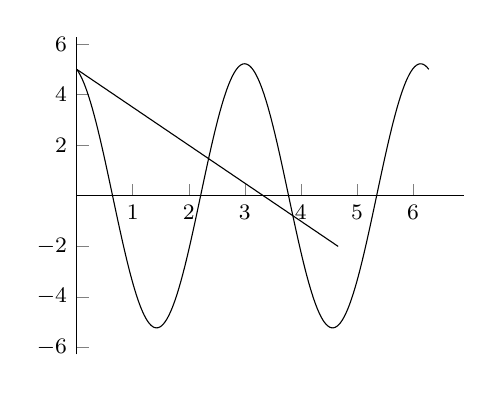
\begin{tikzpicture}
\begin{axis}[small,axis lines*=middle,xmin=0]
\addplot[domain=0:2*pi,samples=200]{5*cos(2*x*180/pi)-1.5*sin(2*x*180/pi)};
\addplot[] plot coordinates {(0,5) (4.666,-2)};
\end{axis}
\end{tikzpicture}
\caption{مثال \حوالہ{مثال_سادہ_دو_درجی_ابتدائی_قیمت_الف} کا مخصوص حل۔}
\label{شکل_مثال_سادہ_دو_درجی_ابتدائی_قیمت_الف}
\end{figure}
\انتہا{مثال}
%===================

درج بالا مثال میں \عددی{y_1} اور \عددی{y_2} ایسے تفاعل تھے جن سے حاصل عمومی حل ابتدائی معلومات پر پورا اترتا تھا۔آئیں اب دو آپس میں راست تناسب حل لیتے ہوئے عمومی حل  لکھیں، مثلاً \عددی{y_1=\cos 2x} اور \عددی{y_2=k\cos 2x} لیتے ہوئے
\begin{align*}
y=c_1\cos 2x+c_2 k\cos 2x=(c_1+c_2k)\cos 2x=c_3\cos 2x
\end{align*}
عمومی حل لکھتے ہیں۔اس مساوات میں ایک عدد اختیاری مستقل \عددی{c_3} پایا جاتا ہے جو دونوں ابتدائی قیمتوں پر پورا اترنے کے لئے نا کافی ہے۔یوں ہم دیکھتے ہیں کہ عمومی حل لکھتے ہوئے ایسے موزوں حل کا خطی میل لیا جاتا ہے جو آپس میں راست تناسبی نہ ہوں۔

 آپ نے یہ بھی دیکھ لیا ہو گا کہ عمومی حل میں استعمال ہونے والے موزوں حل \عددی{y_1} اور \عددی{y_2} انفرادی طور پر دونوں ابتدائی معلومات پر پورا نہیں اتر سکتے البتہ ان کا خطی میل دونوں ابتدائی معلومات پر پورا اترتا ہے۔یہی عمومی حل کی اہمیت کی وجہ ہے۔
%===========================

\ابتدا{تعریف}\quad عمومی حل، اساس اور مخصوص حل کے تعریف\\
کھلے وقفہ \عددی{I} پر سادہ تفرقی مساوات \حوالہ{مساوات_سادہ_متجانس_دو_درجی_تعریف} کا عمومی حل مساوات \حوالہ{مساوات_سادہ_دو_درجی_عمومی_حل_الف} دیتا ہے جہاں \عددی{I} پر \عددی{y_1} اور \عددی{y_2} مساوات  \حوالہ{مساوات_سادہ_متجانس_دو_درجی_تعریف} کے  (آپس میں) غیر تناسبی حل اور \عددی{c_1}، \عددی{c_2} اختیاری مستقل ہیں۔فاصلہ \عددی{I} پر \عددی{y_1} اور \عددی{y_2} مساوات \حوالہ{مساوات_سادہ_متجانس_دو_درجی_تعریف} کی \اصطلاح{اساس}\فرہنگ{اساس!حل}\حاشیہب{basis}\فرہنگ{basis!of solutions} حل کہلاتے ہیں۔

کھلے وقفہ \عددی{I} پر سادہ تفرقی مساوات \حوالہ{مساوات_سادہ_متجانس_دو_درجی_تعریف} کا مخصوص حل مساوات \حوالہ{مساوات_سادہ_دو_درجی_عمومی_حل_الف} میں \عددی{c_1} اور \عددی{c_2} کی جگہ مخصوص قیمتیں پر کرنے سے حاصل ہوتا ہے۔
\انتہا{تعریف}
%============================

کھلے وقفہ کی تعریف حصہ \حوالہ{حصہ_حل_کا_تصور_سادہ_اول} میں دی گئی ہے۔ \عددی{y_1} اور \عددی{y_2} اس صورت  تناسبی تصور کئے جاتے ہیں  جب پورے \عددی{I} پر
\begin{align}
(a)\quad y_1=ky_2 \quad \text{یا} \quad  (b) \quad y_2=ly_1
\end{align} 
ہو، جہاں \عددی{k} اور \عددی{l} اعداد ہیں جو صفر بھی ہو سکتے ہیں۔(یہاں توجہ رکھیں: \عددی{a} اس صورت \عددی{b} کے مترادف ہے جب \عددی{k \ne 0} ہو۔)

آئیں اساس کی تعریف ذرہ مختلف اور عمومی اہمیت کے حامل طریقے سے بیان کریں۔  وقفہ \عددی{I} پر معین \عددی{y_1} اور \عددی{y_2}، وقفہ \عددی{I}  پر، اس صورت \اصطلاح{خطی طور غیر تابع}\فرہنگ{خطی طور! غیر تابع}\حاشیہب{linearly independent}\فرہنگ{linearly independent} کہلاتے ہیں جب پورے وقفے پر
\begin{align}\label{مساوات_سادہ_دو_درجی_خطی_طور_غیر_تابع_الف}
k_1 y_1+k_2 y_2=0
\end{align}
سے مراد 
\begin{align}
k_1=0, \quad k_2=0
\end{align}
ہو۔\عددی{k_1} اور \عددی{k_2} میں سے کم از کم ایک کی قیمت صفر کے برابر نہ ہونے کی صورت میں مساوات \حوالہ{مساوات_سادہ_دو_درجی_خطی_طور_غیر_تابع_الف} پر پورا اترتے ہوئے حل \عددی{y_1} اور \عددی{y_2} \اصطلاح{خطی طور تابع}\فرہنگ{خطی طور!تابع}\حاشیہب{linearly dependent}\فرہنگ{linearly dependent} کہلاتے ہیں۔اگر \عددی{k_1 \ne 0} ہو تب ہم مساوات \حوالہ{مساوات_سادہ_دو_درجی_خطی_طور_غیر_تابع_الف} کو \عددی{k_1} سے تقسیم کرتے ہوئے \عددی{y_1=-\tfrac{k_2}{k_1}y_2} لکھ سکتے ہیں جو تناسبی رشتہ ہے۔اسی طرح \عددی{k_2 \ne 0} کی صورت میں \عددی{y_2=-\tfrac{k_1}{k_2}y_1} لکھا جا سکتا ہے جو تناسبی رشتے کو ظاہر کرتی ہے۔
\begin{align}
y_1=k y_2,\quad y_2=l y_1 \quad \quad  \text{\RL{پورے کھلے وقفے $I$ پر}}
\end{align}
اس کے برعکس خطی طور غیر تابعیت کی صورت میں ہم مساوات \حوالہ{مساوات_سادہ_دو_درجی_خطی_طور_غیر_تابع_الف} کو \عددی{k_1} (یا \عددی{k_2}) سے تقسیم نہیں کر سکتے لہٰذا  تناسبی رشتہ حاصل نہیں کیا جا سکتا۔ (درج بالا مساوات میں \عددی{k=-\tfrac{k_2}{k_1}} اور \عددی{l=-\tfrac{k_1}{k_2}} لکھے گئے ہیں۔\عددی{k} یا (اور) \عددی{l} صفر بھی ہو سکتے ہیں۔)اس طرح اساس کی (درج ذیل) قدر مختلف تعریف حاصل ہوتی ہے۔
%=====================

\ابتدا{تعریف}\quad اساس کی قدر مختلف تعریف\\
کھلے وقفے \عددی{I} پر مساوات \حوالہ{مساوات_سادہ_دو_درجی_خطی_طور_غیر_تابع_الف} کا خطی طور غیر تابع حل   مساوات \حوالہ{مساوات_سادہ_دو_درجی_خطی_طور_غیر_تابع_الف} کے حل کا \اصطلاح{اساس}\فرہنگ{اساس}\فرہنگ{basis} ہے۔
\انتہا{تعریف}
%======================

اگر کسی کھلے وقفے \عددی{I} پر  مساوات \عددی{مساوات_سادہ_متجانس_دو_درجی_تعریف} کے  عددی سر \عددی{p} اور \عددی{q} استمراری تفاعل ہوں تب اس وقفے پر مساوات \عددی{مساوات_سادہ_متجانس_دو_درجی_تعریف}  کا عمومی حل موجود ہے۔مساوات \حوالہ{مساوات_سادہ_دو_درجی_ابتدائی_قیمتیں} میں دیے ابتدائی معلومات استعمال کرتے ہوئے اس عمومی حل سے  مخصوص حل حاصل ہو گا۔ وقفہ \عددی{I} پر مساوات  کے تمام حل یہی عمومی مساوات دے گا لہٰذا ایسی صورت میں مساوات کا کوئی \اصطلاح{نادر}\فرہنگ{نادر!حل}\حاشیہب{singular solution}\فرہنگ{singular solution} حل موجود نہیں ہے (نادر حل کو عمومی حل سے حاصل نہیں کیا جا سکتا ہے۔ یہاں سوال \حوالہ{سوال_سادہ_اول_نادر_حل_الف} سے رجوع کریں)۔ ان تمام حقائق کی وضاحت جلد کی جائے گی۔
%=======================

\ابتدا{مثال}\quad اساس، عمومی اور مخصوص حل\\
\عددی{\cos 2x} اور \عددی{\sin 2x} تمام \عددی{x} پر مثال \حوالہ{مثال_سادہ_دو_درجی_ابتدائی_قیمت_الف} کے تفرقی مساوات \عددی{y''+4y=0} کے حل کی اساس ہیں۔ایسا اس لئے ہے کہ \عددی{\tfrac{\cos 2x}{\sin 2x} \ne c} اور \عددی{\tfrac{\sin 2x}{\cos 2x} \ne 0} ہیں جہاں \عددی{c} مستقل ہے۔اس مثال میں ابتدائی معلومات استعمال کرتے ہوئے عمومی حل سے مخصوص حل \عددی{y=5\cos 2x-1.5\sin 2x} حاصل کیا گیا تھا۔
\انتہا{مثال}
%============================
\ابتدا{مثال}
پر کرتے ہوئے ثابت کریں کہ \عددی{y_1=e^{2x}} اور \عددی{y_2=e^{-2x}} سادہ تفرقی مساوات \عددی{y''-4y=0} کے حل ہیں۔یوں درج ذیل ابتدائی قیمت مسئلے کو حل کریں۔
\begin{align*}
y''-4y=0, \quad y(0)=2, \, y'(0)=1
\end{align*}

حل:چونکہ \عددی{y_1''-4y_1=(e^{2x})''-4e^{2x}=4e^{2x}-4e^{2x}=0} اور \عددی{y_2''-4y_2=(e^{-2x})''-4e^{-2x}=4e^{2x}-4e^{2x}=0}  ہیں لہٰذا \عددی{y_1} اور \عددی{y_2} دیے گئے تفرقی مساوات کے حل ہیں۔چونکہ \عددی{\tfrac{e^{2x}}{e^{-2x}} \ne c} ہے جہاں \عددی{c} مستقل کو ظاہر کرتا ہے  لہٰذا دونوں حل غیر متناسب ہیں اور یوں \عددی{e^{2x}} اور \عددی{e^{-2x}} پورے \عددی{x} پر  حل کا  اساس ہے۔اساس کو استعمال کرتے ہوئے عمومی حل لکھتے ہیں۔
\begin{align*}
y=c_1e^{2x}+c_2e^{-2x}
\end{align*}
عمومی حل اور عمومی حل کے تفرق میں ابتدائی قیمتیں پر کرتے ہوئے مستقل \عددی{c_1} اور \عددی{c_2} حاصل کرتے ہیں۔
\begin{align*}
y(0)=c_1e^{0}+c_2e^{0}=c_1+c_2=2, \quad y'=2c_1e^{2x}-2c_2e^{-2x}, \quad y'(0)=2c_1-2c_2=1
\end{align*}
دو عدد \اصطلاح{ہمزاد مساوات}\فرہنگ{ہمزاد مساوات}\فرہنگ{مساوات!ہمزاد}\حاشیہب{simultaneous equations}\فرہنگ{simultaneous equations} \عددی{c_1+c_2=2} اور \عددی{2c_1-2c_2=1} کو آپس میں حل کرتے ہوئے \عددی{c_1=\tfrac{3}{4}} اور \عددی{c_2=\tfrac{5}{4}} ملتے ہیں جس سے مخصوص حل لکھا جا سکتا ہے۔
\begin{align*}
y=\frac{3}{4}e^{2x}+\frac{5}{4}e^{-2x}
\end{align*}
\انتہا{مثال}
%=========================

\جزوحصہء{ایک حل معلوم ہونے کی صورت میں اساس دریافت کرنا۔ تخفیف درجہ}\شناخت{حصہ_سادہ_دو_درجی_تخفیف_درجہ}
بعض اوقات ایک حل با آسانی حاصل ہو جاتا ہے۔دوسرا خطی طور غیر تابع حل یک درجی سادہ تفرقی مساوات کے حل سے حاصل کیا جا سکتا ہے۔ اس کو \اصطلاح{تخفیف درجہ}\فرہنگ{تخفیف!درجہ}\فرہنگ{درجہ!تخفیف}\حاشیہب{reduction of order}\فرہنگ{reduction!order}\فرہنگ{order!reduction} کی ترکیب\حاشیہد{یہ ترکیب یوسف لوئی لیگرینج (1736-1813) نے دریافت کی۔} کہتے ہیں۔ اس ترکیب کی مثال دیکھنے کے بعد اس کی عمومی اطلاق پر غور کرتے ہیں۔

%========================
\ابتدا{مثال}\شناخت{مثال_سادہ_دو_تخفیف_درجہ}\quad ایک حل جانتے ہوئے تخفیف درجہ۔اساس\\
درج ذیل سادہ تفرقی مساوات کے اساس حل دریافت کریں۔
\begin{align*}
x^2y''-xy'+y=0
\end{align*}

کل:دیے گئے مساوات کے معائنے سے ایک حل \عددی{y_1=x} لکھا جا سکتا ہے چونکہ یوں \عددی{y_1''=0} ہو گا لہٰذا تفرقی مساوات کا پہلا جزو صفر ہو جاتا ہے  اور \عددی{y_1'=1} ہو گا جس سے مساوات کے دوسرے اور تیسرے اجزاء کا مجموعہ صفر ہو جاتا ہے۔ اس ترکیب میں دوسرے حل کو \عددی{y_2=uy_1} لکھ کر دیے گئے تفرقی مساوات میں
\begin{align*}
y_2=uy_1=ux, \quad y_2'=u'x+u, \quad y_2''=u''x+2u'
\end{align*}
 پر کرتے ہیں۔
\begin{align*}
x^2(u''x+2u')-x(u'x+u)+ux=0
\end{align*}
درج بالا کو ترتیب دیتے ہوئے  \عددی{xu} اور \عددی{-xu} آپس میں کٹ جاتے ہیں اور \عددی{x^3u''+x^2u'=0} رہ جاتا ہے جس کو \عددی{x^2} سے تقسیم کرتے ہوئے
\begin{align*}
xu''+u'=0
\end{align*}
ملتا ہے۔اس میں \عددی{u'=v} پر کرتے ہوئے ایک درجی مساوات حاصل ہوتی ہے جس کو علیحدگی متغیرات کے ترکیب سے حل کرتے ہیں۔
\begin{align*}
xv'+v=0,\quad \frac{\dif v}{v}=-\frac{\dif x}{x}, \quad v=\frac{1}{x}
\end{align*}
اس میں واپس \عددی{v=u'} پر کرتے ہوئے تکمل سے \عددی{u} حاصل کرتے ہیں۔
\begin{align*}
v=u'=\frac{1}{x},\quad u=\ln \abs{x}
\end{align*}
یوں \عددی{y_2=x\ln \abs{x}} حاصل ہوتا ہے۔چونکہ \عددی{y_1} اور \عددی{y_2}  کا \اصطلاح{حاصل تقسیم}\فرہنگ{حاصل تقسیم} مستقل نہیں ہے لہٰذا یہ حل خطی طور غیر تابع ہیں اور یوں اساس حل \عددی{y_1=x}، \عددی{y_2=x\ln \abs{x}} ہے۔دونوں بار تکمل لیتے ہوئے تکمل کا مستقل نہیں لکھا گیا چونکہ ہمیں اساس درکار ہے۔عمومی مساوات لکھتے وقت مستقل لکھنا ضروری ہو گا۔
\انتہا{مثال}
%======================== 

اس مثال میں ہم نے \اصطلاح{تخفیف درجہ} کی ترکیب متجانس خطی سادہ تفرقی مساوات 
\begin{align}\label{مساوات_سادہ_دو_درجی_متجانس_تخفیف_الف}
y''+p(x)y'+q(x)y=0
\end{align}
پر استعمال کی۔درج بالا مساوات کو معیاری صورت میں لکھا گیا ہے جہاں پہلا جزو \عددی{y''} ہے جس کا عددی سر اکائی کے برابر ہے۔نیچے اخذ کلیات مساوات کی معیاری صورت کے لئے حاصل کئے گئے ہیں۔تصور کریں کہ کھلے وقفہ \عددی{I} پر ہمیں مساوات \حوالہ{مساوات_سادہ_دو_درجی_متجانس_تخفیف_الف} کا ایک عدد حل \عددی{y_1} معلوم ہے اور ہم حل کا اساس جاننا چاہتے ہیں۔ اس کی خاطر ہمیں \عددی{I} پر خطی طور غیر تابع دوسرا حل \عددی{y_2} درکار ہے۔  دوسرا حل حاصل کرنے کی خاطر ہم
\begin{align*}
y=y_2=uy_1, \quad y'=y_2'=u'y_1+uy_1',\quad y''=y_2''=u''y_1+2u'y_1'+uy_1''
\end{align*}
کو مساوات \حوالہ{مساوات_سادہ_دو_درجی_متجانس_تخفیف_الف} میں پر کرتے ہوئے 
\begin{align*}
(u''y_1+2u'y_1'+uy_1'')+p(u'y_1+uy_1')+q(uy_1)=0
\end{align*}
\عددی{u''}، \عددی{u'} اور \عددی{u} کے عددی سر اکٹھے کرتے ہیں۔
\begin{align*}
u''y_1+u'(2y_1'+py_1')+u(y_1''+py_1'+qy_1)=0
\end{align*}
چونکہ \عددی{y_1} مساوات \حوالہ{مساوات_سادہ_دو_درجی_متجانس_تخفیف_الف} کا حل ہے لہٰذا آخری قوسین صفر کے برابر ہے لہٰذا
\begin{align*}
u''y_1+u'(2y_1'+py_1')=0
\end{align*}
حاصل ہوتا ہے۔ اس کو  \عددی{y_1} سے تقسیم کرتے ہوئے \عددی{u'=v} پر کرنے سے \اصطلاح{تخفیف شدہ}\فرہنگ{تخفیف شدہ}\حاشیہب{reduced}\فرہنگ{reduced} ایک درجی مساوات حاصل ہوتی ہے۔
 \begin{align*}
v'+\left(\frac{2y_1'}{y_1}+p\right)v=0
\end{align*}
علیحدگی متغیرات کے بعد تکمل لینے سے
\begin{align*}
\frac{\dif v}{v}=-\left(\frac{2y_1'}{y_1}+p\right) \dif x, \quad \ln \abs{v}=-2\ln \abs{y_1}-\int p \dif x
\end{align*}
یعنی
\begin{align}
v=\frac{1}{y_1^2}e^{-\int p\dif x}
\end{align}
ملتا ہے۔چونکہ \عددی{v=u'} کے برابر ہے لہٰذا دوسرا حل
\begin{align}
y_2=y_1u=y_1 \int v \dif x
\end{align}
ہو گا۔حاصل تقسیم \عددی{\tfrac{y_2}{y_1}=u=\int p\dif x} مستقل مقدار نہیں ہو سکتا چونکہ \عددی{v>0} ہے لہٰذا \عددی{y_1} اور \عددی{y_2} اساس حل ہیں۔

متجانس خطی دو درجی مساوات سے ایک درجی مساوات کا حصول ہم دیکھ چکے۔ آئیں تخفیف درجہ کے دو مثال دیکھیں جو خطی مساوات اور غیر خطی مساوات پر لاگو کی جا سکتی ہیں۔
%============================
\ابتدا{مثال}
دو درجی خطی یا غیر خطی مساوات \عددی{F(x,y,y',y'')} میں \عددی{y} صریحاً نہیں پایا جاتا۔ اس سے ایک درجی مساوات حاصل کریں۔

حل:چونکہ \عددی{y} صریحاً نہیں پایا جاتا لہٰذا اس کو \عددی{F(x,y',y'')} لکھ سکتے ہیں جس میں \عددی{z=y'} پر کرتے ہوئے ایک درجی مساوات \عددی{F(x,z,z')} حاصل ہوتی ہے۔ایک درجی مساوات کے حل کے تکمل سے \عددی{y} حاصل ہو گا۔
\انتہا{مثال} 
%=============================
\ابتدا{مثال}
دو درجی خطی یا غیر خطی مساوات \عددی{F(x,y,y',y'')} میں \عددی{x} صریحاً نہیں پایا جاتا۔ اس سے ایک درجی مساوات حاصل کریں۔

حل:چونکہ \عددی{x} صریحاً نہیں پایا جاتا لہٰذا اس کو \عددی{F(y,y',y'')} لکھ سکتے ہیں۔ہم \عددی{z=y'=\tfrac{\dif y}{\dif x}} لیتے ہیں۔یوں \اصطلاح{زنجیری تفرق}\فرہنگ{زنجیری تفرق}\حاشیہب{chain rule of differentiation}\فرہنگ{chain rule} سے
\begin{align*}
\frac{\dif z}{\dif y}=\frac{\dif^{\,2} y}{\dif x^2} \frac{\dif x}{\dif y}=\frac{y''}{z}
\end{align*}
یعنی
\begin{align*}
y''=z\frac{\dif z}{\dif y}
\end{align*}
لکھا جا سکتا ہے۔\عددی{z} اور \عددی{z_y} کو دیے مساوات میں پر کرتے ہوئے ایک درجی مساوات \عددی{F(y,z,z_y)} ملتی ہے جس کا آزاد متغیرہ \عددی{y} ہے۔
\انتہا{مثال}
%==========================
%============================

\حصہء{سوالات} \quad سوال \حوالہ{سوال_سادہ_دو_درجی_تخفیف_درجہ_الف} تا سوال \حوالہ{سوال_سادہ_دو_درجی_تخفیف_درجہ_ب} سے ایک درجی مساوات حاصل کرتے ہوئے حل کریں۔
%=======================

\ابتدا{سوال}\شناخت{سوال_سادہ_دو_درجی_تخفیف_درجہ_الف}
\begin{align*}
y''-y'=0
\end{align*}

جواب:\عددی{y=c_1e^x+c_2}
\انتہا{سوال}
%===========================
\ابتدا{سوال}
\begin{align*}
xy''+y'=0
\end{align*}

جواب:\عددی{y=c_1\ln \abs{x}+c_2}
\انتہا{سوال}
%====================
\ابتدا{سوال}
\begin{align*}
xy''-2y'=0
\end{align*}

جواب:\عددی{y=c_1x^3+c_2}
\انتہا{سوال}
%====================
\ابتدا{سوال}
\begin{align*}
yy''-(y')^2=0
\end{align*}

جواب:\عددی{y=c_2e^{c_1x}}
\انتہا{سوال}
%====================
\ابتدا{سوال}
\begin{align*}
y''-(y')^3 \cos y=0
\end{align*}

جواب:\عددی{\cos y+c_1y=x+c_2}
\انتہا{سوال}
%====================
\ابتدا{سوال}
\begin{align*}
y''-(y')^2 \cos y=1
\end{align*}

جواب:\عددی{y=\ln \sec(x+c_1)+c_2}
\انتہا{سوال}
%====================
\ابتدا{سوال}\شناخت{سوال_سادہ_دو_درجی_تخفیف_درجہ_ب}
\begin{align*}
x^2y''-2xy'+2y=0, \quad y_1=x^2
\end{align*}

جواب:\عددی{y=c_1x^2+c_2x}
\انتہا{سوال}
%====================

قابل تخفیف سادہ تفرقی مساوات کے استعمال سوالات \حوالہ{سوال_سادہ_دو_درجی_قابل_تخفیف_الف} تا سوال \حوالہ{سوال_سادہ_دو_درجی_قابل_تخفیف_ب} دیتے ہیں۔

\ابتدا{سوال}\شناخت{سوال_سادہ_دو_درجی_قابل_تخفیف_الف}\quad منحنی\\
کارتیسی محدد کے محور سے گزرتی منحنی \عددی{y''+y'=0} کی مرکز پر ڈھلوان اکائی کے برابر ہے۔منحنی کی مساوات حاصل کریں۔

جواب:\عددی{y=1-e^{-x}}
\انتہا{سوال}
%================================
\ابتدا{سوال}\quad لیزم\\
دو مقررہ نقاط سے لٹکی ہوئی زنجیری ڈوری سے بننے والا خم \اصطلاح{لیزم}\فرہنگ{لیزم}\حاشیہب{catenary}\فرہنگ{catenary} کہلاتا ہے جسے مساوات
 \عددیء{y''=k\sqrt{1+y'^2}} کے حل سے حاصل کیا جاتا ہے۔ مستقل \عددی{k} کی قیمت ڈوری کی تناو اور  کمیت پر منحصر ہے۔ڈوری نقطہ \عددی{(1,0)}  اور \عددی{(-1,0)} سے لٹکی ہوئی ہے۔ \عددی{k=1} تصور کرتے ہوئے  لیزم کی مساوات حاصل کریں۔

جواب:زنجیر کے وسط یعنی\عددی{x=0} پر ڈھلوان صفر کے برابر ہے۔یوں \عددی{y=-1+\cosh x} حاصل ہوتا ہے۔
\انتہا{سوال}
%=============================
\ابتدا{سوال}\quad حرکت\\
ایک چھوٹی جسامت کی چیز سیدھی لکیر پر یوں حرکت کرتی ہے کہ اس کی اسراع اور رفتار میں فرق ایک مثبت مستقل \عددی{k} کے برابر رہتی ہے۔فاصلہ \عددی{y(t)} ابتدائی رفتار \عددی{u} اور ابتدائی فاصلہ \عددی{y_0} پر کس طرح منحصر ہے؟

جواب: \عددیء{y=(k+u)e^t+(y_0-u)-k(t+1)}
\انتہا{سوال}
%========================
\ابتدا{سوال}\شناخت{سوال_سادہ_دو_درجی_قابل_تخفیف_ب}\quad حرکت\\
ایک چھوٹی جسامت کی چیز سیدھی لکیر پر یوں حرکت کرتی ہے کہ اس کی اسراع کی قیمت رفتار کی قیمت کے مربع کے برابر رہتی ہے۔فاصلے کی عمومی مساوات حاصل کریں۔

جواب: \عددیء{t=c_1-\ln(t+c_2)}
\انتہا{سوال}
%========================

سوال \حوالہ{سوال_سادہ_دو_درجی_تخفیف_عمومی_الف} تا سوال \حوالہ{سوال_سادہ_دو_درجی_تخفیف_عمومی_ب} میں ثابت کریں کہ دیے گئے تفاعل خطی طور غیر تابع ہیں اور یوں یہ حل کی اساس ہیں۔ان ابتدائی قیمت سوالات کے حل لکھیں۔


%================================
\ابتدا{سوال}\شناخت{سوال_سادہ_دو_درجی_تخفیف_عمومی_الف} 
\begin{align*}
y''+9y=0,\quad y(0)=5, \quad y'(0)=-2; \quad \cos 3x \, \sin 3x
\end{align*}

جواب:\عددی{y=5\cos 3x-\tfrac{2}{3}\sin 3x}
\انتہا{سوال}
%=================
\ابتدا{سوال}
\begin{align*}
y''-2y'+y=0, \quad y(1)=0, \quad y'(1)=1;\quad e^x,\, xe^x
\end{align*}

جواب:\عددی{y=e^{x-1}(x-1)}
\انتہا{سوال}
%=================
\ابتدا{سوال}
\begin{align*}
x^2y''-xy'+y=0, \quad y(1)=3.2, \quad y'(1)=-1.5;\quad x,\, x\ln x
\end{align*}

جواب:\عددی{y=\tfrac{16}{5}x-\tfrac{47}{10} x\ln x}
\انتہا{سوال}
%=================
\ابتدا{سوال}\شناخت{سوال_سادہ_دو_درجی_تخفیف_عمومی_ب}
\begin{align*}
y''+2y'+3y=0, \quad y(0)=2, \quad y'(0)=-3;\quad e^{-x}\cos \sqrt{2}x, \,\, e^{-x}\sin \sqrt{2} x
\end{align*}

جواب:\عددی{y=e^{-x}(2\cos \sqrt{2}x-\tfrac{1}{\sqrt{2}}\sin \sqrt{2}x)}
\انتہا{سوال}
%=================
%==================

\حصہ{مستقل عددی سر والے متجانس خطی سادہ تفرقی مساوات}\شناخت{حصہ_سادہ_دو_درجی_مستقل_عددی_سر}
اب ایسے دو درجی متجانس تفرقی مساوات پر بات کرتے ہیں جن کے عددی سر \عددی{a} اور \عددی{b} مستقل مقدار ہیں۔
\begin{align}\label{مساوات_سادہ_دو_درجی_مستقل_عددی_سر_الف}
y''+ay'+b=0
\end{align} 
یہ مساوات میکانی اور برقی ارتعاش میں اہم کردار ادا کرتی ہے۔قوت نمائی تفاعل \عددی{y=e^{-kx}} کے تفرق سے \عددی{y'=-ke^{-kx}=-ky} یعنی \عددی{y'+ky=0} تفرقی مساوات حاصل ہوتا ہے۔یوں \عددی{y'+ky=0} کا حل \عددی{y=e^{-kx}} ہے۔اس کو دیکھتے ہوئے ہم دیکھنا چاہتے ہیں کہ آیا مساوات \حوالہ{مساوات_سادہ_دو_درجی_مستقل_عددی_سر_الف} کا حل
\begin{align}\label{مساوات_سادہ_دو_درجی_مستقل_عددی_سر_ب}
y=e^{\lambda x}
\end{align}
 ممکن ہے یا نہیں۔یہ جاننے کی خاطر \عددی{y=e^{\lambda x}} اور اس کے تفرق
\begin{align*}
y'=\lambda e^{\lambda x}, \quad y''=\lambda^2 e^{\lambda x}
\end{align*}
 کو  مساوات \حوالہ{مساوات_سادہ_دو_درجی_مستقل_عددی_سر_الف} میں پر کرتے  ہیں۔
\begin{align*}
(\lambda^2+a\lambda+b)e^{\lambda x}=0
\end{align*}  
کسی بھی محدود قیمت کے \عددی{\lambda} اور \عددی{x} کے لئے \عددی{e^{\lambda x}} صفر نہیں ہو گا لہٰذا اس مساوات کے دونوں اطراف صرف اس صورت برابر ہو سکتے ہیں جب \عددی{\lambda} \اصطلاح{امتیازی مساوات}\فرہنگ{امتیازی مساوات}\حاشیہب{characteristic equation}\فرہنگ{characteristic equation}
 \begin{align}\label{مساوات_سادہ_دو_درجی_مستقل_عددی_سر_پ}
\lambda^2+a\lambda+b=0
\end{align}
 کا جذر ہو۔اس \اصطلاح{دو درجی الجبرائی مساوات}\فرہنگ{دو درجی الجبرائی مساوات}\حاشیہب{quadratic equation}\فرہنگ{quadratic equation} کو حل کرتے ہیں۔
\begin{align}\label{مساوات_سادہ_دو_درجی_مستقل_عددی_سر_ت}
\lambda_1=\frac{-a+\sqrt{a^2-4b}}{2}, \quad \lambda_2=\frac{-a-\sqrt{a^2-4b}}{2}
\end{align}
یوں مساوات \حوالہ{مساوات_سادہ_دو_درجی_مستقل_عددی_سر_الف} کے حل
\begin{align}
y_1=e^{\lambda_1 x}, \quad y_2=e^{\lambda_2 x}
\end{align}
ہوں گے۔انہیں مساوات \حوالہ{مساوات_سادہ_دو_درجی_مستقل_عددی_سر_الف} میں پر کرتے ہوئے آپ ثابت کر سکتے ہیں کہ یہی تفرقی مساوات کے حل ہیں۔

دو درجی الجبرائی مساوات \حوالہ{مساوات_سادہ_دو_درجی_مستقل_عددی_سر_پ} کے جذر کی تین ممکنہ قیمتیں ہیں جو \عددی{a^2-4b} کی علامت \عددی{(\mp)}  پر منحصر ہیں۔
\begin{itemize}\label{لسٹ_سادہ_دو_درجی_تین_صورتیں_الف}
\item[پہلی صورت:]
دو منفرد حقیقی جذر \quad $a^2-4c>0$ 
\item[دوسری صورت:]
 دوہرا حقیقی جذر \quad $a^2-4c=0$ 
\item[تیسری صورت:]
 جوڑی دار مخلوط جذر \quad $a^2-4c<0$ 
\end{itemize}
آئیں ان تین صورتوں پر باری باری غور کریں۔
%============================================

\حصہء{پہلی صورت: دو منفرد حقیقی جذر}
اس صورت میں، چونکہ \عددی{y_1} اور \عددی{y_2} کسی بھی وقفے \عددی{I} پر معین ہیں (اور حقیقی ہیں)  اور ان کا حاصل تقسیم مستقل قیمت نہیں ہے لہٰذا کسی بھی وقفے  پر مساوات \حوالہ{مساوات_سادہ_دو_درجی_مستقل_عددی_سر_الف} کے حل کا اساس
\begin{align}
y_1=e^{\lambda_1 x}, \quad y_2=e^{\lambda_2 x}
\end{align}
ہو گا۔یوں تفرقی مساوات کا عمومی حل درج ذیل ہو گا۔
\begin{align}
y=c_1e^{\lambda_1 x}+c_2 e^{\lambda_2 x}
\end{align}
%======================
\ابتدا{مثال}\quad دو حقیقی منفرد جذر\\
مساوات \عددی{y''-4y=0} کا حل حاصل کرتے ہیں۔اس کا امتیازی مساوات \عددی{\lambda^2-4=0} ہے جس کے جذر \عددی{\lambda_1=+2} اور \عددی{\lambda_2=-2}  دو منفرد قیمتیں ہیں۔یوں حل کا اساس \عددی{y_1=e^{2x}} اور \عددی{y_2=e^{-2x}} ہے جن سے تفرقی مساوات کا عمومی حل \عددی{y=c_1e^{2x}+c_2e^{-2x}} لکھا جا سکتا ہے۔
\انتہا{مثال}
%============================
\ابتدا{مثال}\شناخت{مثال_سادہ_دو_درجی_حقیقی_منفرد_جذر_الف}\quad ابتدائی قیمت مسئلہ۔دو حقیقی منفرد جذر\\
درج ذیل ابتدائی قیمت مسئلے کو حل کریں۔
\begin{align*}
y''+y'-6=0,\quad y(0)=-4, \quad y'(0)=5
\end{align*} 
حل: امتیازی مساوات لکھتے ہیں
\begin{align*}
\lambda^2+\lambda-6=0
\end{align*}
جس کے جذر
\begin{align*}
\lambda_1=\frac{-1+\sqrt{1+24}}{2}=2, \quad \lambda_2=\frac{-1-\sqrt{1+24}}{2}=-3,
\end{align*}
ہیں۔ان سے اساس حل \عددی{y_1=e^{2x}}، \عددی{y_2=e^{-3x}} ملتا ہے جس سے عمومی حل حاصل ہوتا ہے۔
\begin{align*}
y=c_1e^{2x}+c_2e^{-3x}
\end{align*}
ابتدائی قیمتیں پر کرتے ہوئے مستقل حاصل کرتے ہیں۔چونکہ \عددی{y'=2c_1e^{2x}-3c_2e^{-3x}} ہے لہٰذا
\begin{align*}
y(0)&=c_1+c_2=-4\\
y'(0)&=2c_1-3c_2=5
\end{align*}
لکھا جائے گا۔ان ہمزاد مساوات کو حل کرتے ہوئے \عددی{c_1=-\tfrac{7}{5}} اور \عددی{c_2=-\tfrac{13}{5}} ملتا ہے جن سے \اصطلاح{مخصوص حل} لکھتے ہیں۔
 \begin{align*}
y=-\frac{7}{5}e^{2x}-\frac{13}{5}e^{-3x}
\end{align*}
مخصوص حل کو شکل \حوالہ{شکل_مثال_سادہ_دو_درجی_حقیقی_منفرد_جذر_الف} میں دکھایا گیا ہے جو ابتدائی قیمتوں پر پورا اترتا ہے۔
%
\begin{figure}
\centering
\begin{tikzpicture}
\begin{axis}[small,xlabel={$x$},ylabel={$y$},ylabel style={rotate=-90},ylabel style={at={(axis description cs:0,1.05)}}]
\addplot[domain=0:1]{-7/5*e^(2*x)-13/5*e^(-3*x)};
\end{axis}
\end{tikzpicture}
\caption{مثال \حوالہ{مثال_سادہ_دو_درجی_حقیقی_منفرد_جذر_الف} کا مخصوص حل۔}
\label{شکل_مثال_سادہ_دو_درجی_حقیقی_منفرد_جذر_الف}
\end{figure}
\انتہا{مثال}
%=============================

\حصہء{دوسری صورت: دوہرا حقیقی جذر}
اگر \عددی{a^2-4c=0} ہو تب مساوات \حوالہ{مساوات_سادہ_دو_درجی_مستقل_عددی_سر_ت} سے \عددی{\lambda_1=\lambda_2=-\tfrac{a}{2}} ملتا ہے جو واحد حل
\begin{align*}
y_1=e^{-\frac{a}{2}x}
\end{align*}
دیتا ہے۔ ہمیں اساس کے لئے دو حل درکار ہیں۔دوسرا حل \اصطلاح{تخفیف درجہ} کی ترکیب سے حاصل کیا جائے گا۔اس ترکیب پر بحث ہو چکی ہے۔یوں ہم دوسرا حل \عددی{y_2=uy_1} تصور کرتے ہیں۔مساوات \حوالہ{مساوات_سادہ_دو_درجی_مستقل_عددی_سر_الف} میں
\begin{align*}
y_2=uy_1,\quad y_2'=u'y_1+uy_1',\quad y''=u''y_1+2u'y_1'+uy_1''
\end{align*}
پر کرتے
\begin{align*}
(u''y_1+2u'y_1'+uy_1'')+a(u'y_1+uy_1')+b(uy_1)=0
\end{align*}
ہوئے \عددی{u''}، \عددی{u'} اور \عددی{u} کے عددی سر اکٹھے کرتے ہیں۔
\begin{align}\label{مساوات_سادہ_دو_درجی_دوہرا_جذر_الف}
u'' y_1+u'(2y_1'+ay_1)+u(y_1''+ay_1'+by_1)=0
\end{align}
چونکہ \عددی{y_1} تفرقی مساوات کا حل ہے لہٰذا آخری قوسین صفر کے برابر  ہے۔اب پہلی قوسین پر غور کرتے ہیں۔چونکہ \عددی{y_1=e^{-\tfrac{a}{2}x}} لہٰذا \عددی{y_1'=-\tfrac{a}{2}y_1} ہو گا۔ان قیمتوں کو پہلی قوسین میں پر کرتے
\begin{align*}
2y_1'+ay_1=2(-\frac{a}{2}y_1)+ay_1=0
\end{align*}
ہوئے یہ قوسین بھی صفر کے برابر حاصل ہوتی ہے۔یوں مساوات \حوالہ{مساوات_سادہ_دو_درجی_دوہرا_جذر_الف} سے \عددی{u''y_1=0} یعنی \عددی{u''=0} حاصل ہوتا ہے۔دو مرتبہ تکمل لیتے ہوئے \عددیء{u=c_1 x+c_2} ملتا ہے۔دوسرا خطی طور غیر تابع حل \عددی{y_2=uy_1} حاصل کرتے ہوئے ہم \عددی{c_1=1} اور \عددی{c_2=0} چن سکتے ہیں جن سے
 \عددی{u=x} اور \عددی{y_2=xy_1} حاصل ہوتے ہیں۔چونکہ \عددی{y_1} اور حاصل کردہ \عددی{y_2=xy_1} کا حاصل تقسیم مستقل مقدار نہیں ہے لہٰذا یہ دونوں خطی طور غیر تابع ہیں اور انہیں اساس لیا جا سکتا ہے۔یوں دوہرے جذر کی صورت میں کسی بھی وقفے پر مساوات \حوالہ{مساوات_سادہ_دو_درجی_مستقل_عددی_سر_الف} کے حل کا اساس 
\begin{align*}
y_1=e^{-\frac{a}{2}x}, \quad y_2=xe^{-\frac{a}{2}x}
\end{align*}
اور عمومی حل درج ذیل ہو گا۔
\begin{align}
y=(c_1 +c_2 x)e^{-\frac{a}{2}x}
\end{align}
%============================
\ابتدا{مثال}\quad دوہرے جذر کی صورت میں عمومی حل\\
سادہ تفرقی مساوات \عددی{y''+10y'+25=0} کا امتیازی مساوات \عددی{\lambda^2+10\lambda+25=0} ہے جس کو \عددی{(\lambda+5)^2=0} لکھ کر دوہرا جذر \عددی{\lambda_1=\lambda_2=-5} حاصل ہوتا ہے۔یوں تفرقی مساوات کے حل کا اساس \عددی{y_1=e^{-5x}}، \عددی{y_2=xe^{-5x}} اور اس کا عمومی حل \عددی{y=(c_1+c_2 x)e^{-5x}} ہے۔

\انتہا{مثال}
%===================================
\ابتدا{مثال}\شناخت{مثال_سادہ_دو_درجی_حقیقی_دوہرا_جذر}\quad دوہرے جذر کی صورت میں مخصوص حل کا حصول\\
دیے گئے تفرقی مساوات کا مخصوص حل دریافت کریں۔
\begin{align*}
y''+0.2y'+0.01y=0, \quad y(0)=10, \quad y'(0)=-4
\end{align*}

حل: امتیازی مساوات \عددی{\lambda^2+0.2\lambda+0.01=0} یعنی \عددی{(\lambda+0.1)^2=0} سے  \عددی{\lambda_1=\lambda_2=-0.1} دوہرا جذر حاصل ہوتا ہے جس سے عمومی حل لکھتے ہیں۔
\begin{align*}
y=(c_1+c_2 x)e^{-0.1x}
\end{align*}
عمومی حل کا جذر لکھتے ہیں جو مخصوص حل کے حصول میں درکار ہے۔
\begin{align*}
y'=c_2 e^{-0.1x}-0.1(c_1+c_2 x)e^{-0.1x}
\end{align*}
عمومی حل اور عمومی حل کے تفرق  میں ابتدائی قیمتیں پر کرتے ہوئے \عددی{c_1} اور \عددی{c_2} حاصل کرتے ہیں۔
\begin{align*}
y(0)&=c_1=10\\
y'(0)&=c_2-0.1 c_1=-4, \quad c_2=-3
\end{align*}
یوں مخصوص حل درج ذیل ہو گا۔
\begin{align*}
y=(10-3x)e^{-0.1x}
\end{align*}
مخصوص حل کو شکل \حوالہ{شکل_مثال_سادہ_دو_درجی_حقیقی_دوہرا_جذر} میں دکھایا گیا ہے۔
\begin{figure}
\centering
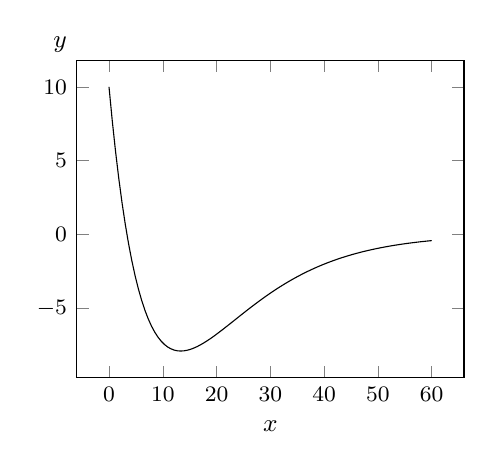
\begin{tikzpicture}
\begin{axis}[small,xlabel={$x$},ylabel={$y$},ylabel style={rotate=-90},ylabel style={at={(axis description cs:0,1.05)}}]
\addplot[domain=0:60,samples=100]{(10-3*x)*e^(-0.1*x)};
\end{axis}
\end{tikzpicture}
\caption{مثال \حوالہ{مثال_سادہ_دو_درجی_حقیقی_دوہرا_جذر} کا مخصوص حل۔}
\label{شکل_مثال_سادہ_دو_درجی_حقیقی_دوہرا_جذر}
\end{figure}
\انتہا{مثال}
%=============================

\حصہء{تیسری صورت: مخلوط جوڑی دار جذر}
امتیازی مساوات \حوالہ{مساوات_سادہ_دو_درجی_مستقل_عددی_سر_پ} میں \عددی{a^2-4c} کی قیمت منفی ہونے کی صورت میں مخلوط جوڑی دار
 جذر \عددی{\lambda=-\tfrac{a}{2}\mp i\omega} ملتے ہیں جہاں \عددی{\omega^2=b-\tfrac{a^2}{4}} کے برابر ہے۔ان سے مخلوط اساس لکھتے ہیں۔
\begin{align}\label{مساوات_سادہ_دو_درجی_مخلوط_اساس_الف}
y_{m1}=e^{(-\frac{a}{2}+i\omega)x},\quad y_{m2}=e^{(-\frac{a}{2}-i\omega)x}
\end{align}
اس مخلوط اساس سے حقیقی اساس حاصل کیا جائے گا۔ایسا کرنے کی خاطر ریاضی کے چند کلیات پر غور کرتے ہیں۔تفاعل \عددی{e^z}، جہاں \عددی{z=x+iy} مخلوط عدد ہے  جبکہ \عددی{x} اور \عددی{y} حقیقی اعداد ہیں، کو درج ذیل لکھا جا سکتا ہے۔
\begin{align*}
e^z=e^{x+iy}=e^xe^{iy}
\end{align*}
\عددی{e^{iy}} کی \اصطلاح{مکلارن تسلسل}\فرہنگ{مکلارن تسلسل}\فرہنگ{تسلسل!مکلارن}\حاشیہب{Maclaurin series}\فرہنگ{Maclaurin series} لکھ کر حقیقی اجزاء اور خیالی اجزاء کو علیحدہ علیحدہ قوسین میں اکٹھے کرتے ہیں۔یہاں \عددی{i^2=-1}، \عددی{i^3=-i}، \عددی{i^4=1} لئے گئے ہیں۔
\begin{align*}
e^{iy}&=1+\frac{iy}{1!}+\frac{(iy)^2}{2!}+\frac{(iy)^3}{3!}+\frac{(iy)^4}{4!}+\frac{(iy)^5}{5!}\cdots\\
&=\left(1-\frac{y^2}{2!}+\frac{y^4}{4!}-+\cdots\right) +i\left(\frac{y}{1!}-\frac{y^3}{3!}+\frac{y^5}{5!}-+\cdots\right)\\
&=\cos y+i\sin y
\end{align*}
آخری قدم پر آپ تسلی کر لیں کہ پہلی قوسین \عددی{\cos y} کی مکلارن تسلسل دیتی ہے جبکہ دوسری قوسین \عددی{\sin y} کی مکلارن تسلسل دیتی ہے۔ آپ اس کتاب میں آگے پڑھیں گے کہ درج بالا تسلسل میں اجزاء کی ترتیب بدلی جا سکتی ہے۔یوں ہم \اصطلاح{یولر مساوات}\فرہنگ{یولر مساوات}\حاشیہب{Euler equation}\فرہنگ{Euler equation}  
 \begin{align}\label{مساوات_سادہ_دو_درجی_یولر_مساوات_الف}
e^{iy}=\cos y+i\sin y
\end{align}
حاصل کرنے میں کامیاب ہوئے ہیں۔آپ دیکھ سکتے ہیں کہ
\begin{align}\label{مساوات_سادہ_دو_درجی_یولر_مساوات_ب}
e^{-iy}=\cos (-y)+i\sin (-y)=\cos y-i\sin y
\end{align}
مساوات \حوالہ{مساوات_سادہ_دو_درجی_یولر_مساوات_الف} اور مساوات \حوالہ{مساوات_سادہ_دو_درجی_یولر_مساوات_ب} کو جمع اور تفریق کرتے ہوئے درج ذیل کلیات حاصل ہوتے ہیں۔
\begin{align}
\cos y=\frac{e^{iy}+e^{-iy}}{2}, \quad \sin y=\frac{e^{iy}-e^{-iy}}{2i}
\end{align}
ہو گا۔یہ سب جاننے کے بعد آئیں مساوات \حوالہ{مساوات_سادہ_دو_درجی_مخلوط_اساس_الف} میں دیے مخلوط اساس پر دوبارہ غور کریں۔
\begin{align*}
y_{m1}&=e^{(-\frac{a}{2}+i\omega)x}=e^{-\frac{a}{2}x}e^{i\omega x}=e^{-\frac{a}{2}x} (\cos \omega x+i\sin \omega x)\\
y_{m2}&=e^{(-\frac{a}{2}-i\omega)x}=e^{-\frac{a}{2}x}e^{-i\omega x}=e^{-\frac{a}{2}x} (\cos \omega x-i\sin \omega x)
\end{align*}
چونکہ اساس کے اجزاء کو مستقل (حقیقی یا خیالی یا مخلوط) سے ضرب دے کر جمع کرتے ہوئے نیا حل حاصل کیا جا سکتا ہے لہٰذا ہم درج بالا دونوں اجزاء کو مستقل \عددی{\tfrac{1}{2}} سے ضرب دے کر جمع کرتے ہوئے ایک نیا اور حقیقی حل \عددی{y_1} دریافت کرتے ہیں۔
\begin{align*}
y_1=\frac{1}{2}y_{m1}+\frac{1}{2}y_{m2}=e^{-\frac{a}{2}x} \cos \omega x
\end{align*}
اسی طرح مخلوط اساس کے پہلے جزو  کو مستقل \عددی{\tfrac{1}{2i}} اور دوسرے جزو کو مستقل \عددی{-\tfrac{1}{2i}} سے ضرب دیتے ہوئے جمع کر کے نیا اور حقیقی حل \عددی{y_2} حاصل کرتے ہیں۔
\begin{align*}
y_2=\frac{1}{2i}y_{m1}-\frac{1}{2i}y_{m2}=e^{-\frac{a}{2}x} \sin \omega x
\end{align*}
درج بالا حاصل کردہ حقیقی تفاعل 
\begin{align}\label{مساوات_سادہ_دو_درجی_مخلوط_اساس_ب}
y_1=e^{-\frac{a}{2}x} \cos \omega x\quad y_2=e^{-\frac{a}{2}x} \sin \omega x
\end{align}
 کو از خود حل کا اساس تصور کیا جا سکتا ہے۔ یہاں غور کریں کہ ہم نے مخلوط جذر \عددی{\lambda=(-\tfrac{a}{2}\mp i \omega)x} سے حقیقی اساس  (مساوات \حوالہ{مساوات_سادہ_دو_درجی_مخلوط_اساس_ب}) حاصل کیا ہے۔ اس حقیقی اساس کو استعمال کرتے ہوئے عمومی حل لکھتے ہیں۔
\begin{align}
y=e^{-\frac{a}{2}x} (c_1 \cos \omega x+c_2 \sin \omega x)
\end{align}

 %==============================
%===============================
\ابتدا{مثال}\شناخت{مثال_سادہ_دو_درجی_مخلوط_جذر_الف}\quad مخلوط جذر، ابتدائی قیمت مسئلہ\\
درج ذیل ابتدائی قیمت مسئلے کو حل کریں۔
\begin{align*}
y''+0.36y'+9.0324y=0,\quad y(0)=0, \quad y'(0)=3
\end{align*}

حل:امتیازی مساوات \عددی{\lambda^2+0.36\lambda+9.0324=0} کے مخلوط جذر \عددی{\lambda=-0.18+\mp i3} ہیں لہٰذا عمومی حل
\begin{align*}
y=e^{-0.18x}(c_1 \cos 3x+c_2 \sin 3x)
\end{align*}
ہو گا۔مخصوص حل حاصل کرنے کی خاطر \عددی{c_1} اور \عددی{c_2} درکار ہیں جنہیں عمومی مساوات میں ابتدائی معلومات پر کرتے ہوئے حاصل کرتے ہیں۔پہلے ابتدائی معلومات سے
\begin{align*}
y(0)=e^{0}(c_1 \cos 0+c_2 \sin 0)=0, \quad c_1=0
\end{align*}
ملتا ہے۔عمومی حل کے تفرق
\begin{align*}
y'=-0.5e^{-0.5x}(c_1 \cos 3x+c_2 \sin 3x)+e^{-0.5x}(-3c_1 \sin 3x+3c_2 \cos 3x)
\end{align*}
میں دوسری ابتدائی معلومات پر کرتے ہوئے
\begin{align*}
y'=-0.5e^{0}(0 \cos 0+c_2 \sin 0)+e^{0}(0 \sin 0+3c_2 \cos 0)=3, \quad c_2=1
\end{align*}
ملتا ہے۔یوں مخصوص حل درج ذیل ہو گا۔
\begin{align*}
y=e^{-0.18x}\sin 3x
\end{align*}
شکل \حوالہ{شکل_مثال_سادہ_دو_درجی_مخلوط_جذر_الف} میں مخصوص حل دکھایا گیا ہے۔ساتھ ہی ساتھ، نقطہ دار لکیروں سے، سائن نما منحنی کے مثبت چوٹیوں کو چھوتا ہوا \اصطلاح{غلاف}\فرہنگ{غلاف}\حاشیہب{envelope}\فرہنگ{envelope} \عددی{e^{-0.18x}} اور منفی چوٹیوں کو چھوتا ہوا غلاف \عددی{-e^{-0.18x}} بھی دکھائے گئے ہیں۔مخصوص حل (\عددی{x} کو \عددی{t} لیتے ہوئے) \اصطلاح{قصری ارتعاش}\فرہنگ{قصری!ارتعاش}\فرہنگ{ارتعاش!قصری}\حاشیہب{damped oscillations}\فرہنگ{oscillations!damped} کو ظاہر کرتی ہے۔اگر \عددیء{y} فاصلے کو ظاہر کرتی ہو تب یہ میکانی قصری ارتعاش ہو گی اور اگر \عددی{y} برقی رو یا برقی دباو ہو تب یہ برقی قصری ارتعاش ہو گی۔
\begin{figure}
\centering
\begin{tikzpicture}
\begin{axis}[small,xlabel={$x$},ylabel={$y$},ylabel style={rotate=-90},ylabel style ={at={(axis description cs:0,1.05)}}]
\addplot[domain=0:25,samples=300] {e^(-0.18*x)*sin(3*x*180/pi)};
\addplot[dashed,domain=0:25]{e^(-0.18*x)}node[pos=0.15,pin=45:{غلاف}]{};
\addplot[dashed,domain=0:25]{-e^(-0.18*x)};
\end{axis}
\end{tikzpicture}
\caption{مثال \حوالہ{مثال_سادہ_دو_درجی_مخلوط_جذر_الف} کا مخصوص حل۔}
\label{شکل_مثال_سادہ_دو_درجی_مخلوط_جذر_الف}
\end{figure}

\انتہا{مثال}
%================================
\ابتدا{مثال}\quad مخلوط جذر\\
سادہ تفرقی مساوات
\begin{align*}
y''+\omega^2 y=0,\quad \text{\RL{($\omega$\, غیر صفر مستقل ہے)}}
\end{align*}
کا عمومی حل درج ذیل ہے۔
\begin{align*}
y=c_1 \cos \omega x+c_2 \sin \omega x
\end{align*}
\انتہا{مثال}
%================================

\begin{table}
\caption{تین صورتوں کی تفصیل}
\label{جدول_سادہ_دو_درجی_تین_صورتیں}
\centering
\begin{tabular}{rrrl}
صورت& مساوات \حوالہ{مساوات_سادہ_دو_درجی_مستقل_عددی_سر_پ} کے جذر & مساوات \حوالہ{مساوات_سادہ_دو_درجی_مستقل_عددی_سر_الف} کی اساس & مساوات \حوالہ{مساوات_سادہ_دو_درجی_مستقل_عددی_سر_الف} کا عمومی حل\\
\hline
پہلی & منفرد حقیقی \عددی{\lambda_1} ،\عددی{\lambda_2} & \عددی{e^{\lambda_1 x}}، \عددی{e^{\lambda_2 x}} & \عددی{y=c_1 e^{\lambda_1 x}+c_2 e^{\lambda_2 x}}  \\
دوسری& دوہرا جذر \عددی{\lambda=-\frac{a}{2}} & \عددی{e^{-\frac{a}{2}x}}، \عددی{xe^{-\frac{a}{2}x}} &  \عددی{y=(c_1+c_2 x)e^{-\frac{a}{2}x}}\\
تیسری& جوڑی دار مخلوط&   \عددی{e^{-\frac{a}{2}x}\cos\omega x}، & \عددی{y=e^{-\frac{a}{2}x}(c_1 \cos \omega x+c_2 \sin \omega x)}\\
 &  \عددی{\lambda=-\frac{a}{2} \mp i\omega} &\عددی{e^{-\frac{a}{2}x}\sin \omega x}&
\end{tabular}
\end{table}

جدول \حوالہ{جدول_سادہ_دو_درجی_تین_صورتیں} میں درج بالا تین صورتوں کی تفصیل اکٹھی کی گئی ہے۔یہ تین اقسام میکانی ارتعاش یا برقی ارتعاش کو ظاہر کرتی ہیں۔آپ تفرقی مساوات کی قوت یہاں سے جان سکتے ہیں۔آپس میں بالکل مختلف میدانوں (مثلاً میکانی اور برقی) کے مسائل ایک طرز  کی تفرقی مساوات سے ظاہر کئے جا سکتے ہیں۔ 
%====================================
%=====================================

\حصہء{سوالات}
سوال \حوالہ{سوال_سادہ_دو_درجی_مستقل-عددی_سر_الف} تا سوال \حوالہ{سوال_سادہ_دو_درجی_مستقل-عددی_سر_ب} کے عمومی حل حاصل کریں۔انہیں واپس تفرقی مساوات میں پر کرتے ہوئے ان کی درستگی ثابت کریں۔

%==================
\ابتدا{سوال}\شناخت{سوال_سادہ_دو_درجی_مستقل-عددی_سر_الف}
\begin{align*}
y''+4y=0
\end{align*}
جواب:\عددی{y=c_1\cos 2x+c_2 \sin 2x}
\انتہا{سوال}
%========================
\ابتدا{سوال}
\begin{align*}
4y''-9y=0
\end{align*}
جواب:\عددی{y=c_1e^{\frac{3}{2}x}+c_2 e^{-\frac{3}{2}x}}
\انتہا{سوال}
%========================
\ابتدا{سوال}
\begin{align*}
y''+5y'+6y=0
\end{align*}
جواب:\عددی{y=c_1e^{-2x}+c_2e^{-3x}}
\انتہا{سوال}
%========================
\ابتدا{سوال}
\begin{align*}
y''+2\pi y'+\pi^2 y=0
\end{align*}
جواب:\عددی{y=(c_1+c_2 x)e^{-\pi x}}
\انتہا{سوال}
%========================
\ابتدا{سوال}
\begin{align*}
y''-6 y'+9 y=0
\end{align*}
جواب:\عددی{y=(c_1+c_2 x)e^{3x}}
\انتہا{سوال}
%========================
\ابتدا{سوال}
\begin{align*}
4y''-12 y'+9 y=0
\end{align*}
جواب:\عددی{y=(c_1+c_2 x)e^{\tfrac{3}{2}x}}
\انتہا{سوال}
%========================
\ابتدا{سوال}
\begin{align*}
4y''+4 y'-3 y=0
\end{align*}
جواب:\عددی{y=c_1e^{\tfrac{x}{2}}+c_2 e^{-\tfrac{3}{2}x}}
\انتہا{سوال}
%========================
\ابتدا{سوال}
\begin{align*}
y''-5 y'+6 y=0
\end{align*}
جواب:\عددی{y=c_1e^{3x}+c_2e^{2x}}
\انتہا{سوال}
%========================
\ابتدا{سوال}\شناخت{سوال_سادہ_دو_درجی_مستقل-عددی_سر_ب}
\begin{align*}
9y''-30 y'+25 y=0
\end{align*}
جواب:\عددی{y=(c_1+c_2 x)e^{\tfrac{5}{3}x}}
\انتہا{سوال}
%========================

سوال \حوالہ{سوال_سادہ_دو_درجی_مستقل-عددی_سر_پ} تا سوال \حوالہ{سوال_سادہ_دو_درجی_مستقل-عددی_سر_ت} میں اساس سے تفرقی مساوات \عددی{y''+ay'+by=0} حاصل کریں۔

%======================
\ابتدا{سوال}\شناخت{سوال_سادہ_دو_درجی_مستقل-عددی_سر_پ}
\begin{align*}
e^{0.2x}, \quad e^{-0.5x}
\end{align*}
جواب:\عددی{y''+0.3y'-0.1y=0}
\انتہا{سوال}
%=======================
\ابتدا{سوال}
\begin{align*}
e^{-0.66x}, \quad e^{-0.32x}
\end{align*}
جواب:\عددی{y''+0.98y'+0.2112y=0}
\انتہا{سوال}
%=======================
\ابتدا{سوال}
\begin{align*}
\cos (4\pi x), \quad \sin (4\pi x)
\end{align*}
جواب:\عددی{y''+16\pi^2 y=0}
\انتہا{سوال}
%=======================
\ابتدا{سوال}
\begin{align*}
e^{(-2+i3)x}, \quad e^{(-2-i3)x}
\end{align*}
جواب:\عددی{y''+4y''+13y=0}
\انتہا{سوال}
%=======================
\ابتدا{سوال}\شناخت{سوال_سادہ_دو_درجی_مستقل-عددی_سر_ت}
\begin{align*}
e^{-1.7x}\cos 6.2 x, \quad e^{-1.7x}\sin 6.2x
\end{align*}
جواب:\عددی{y''+3.4y''+41.33y=0}
\انتہا{سوال}
%=======================

سوال \حوالہ{سوال_سادہ_دو_درجی_مستقل-عددی_سر_ٹ} تا سوال \حوالہ{سوال_سادہ_دو_درجی_مستقل-عددی_سر_ث} ابتدائی قیمت سوالات ہیں۔ان کے مخصوص حل دریافت کریں۔

%================
\ابتدا{سوال}\شناخت{سوال_سادہ_دو_درجی_مستقل-عددی_سر_ٹ}
\begin{align*}
y''+2y=0,\quad y(0)=5,\quad y'(0)=2
\end{align*}
جواب:\عددی{y=5\cos \sqrt{2} x+\sqrt{2}\sin \sqrt{2} x}
\انتہا{سوال}
%===========================
\ابتدا{سوال}
\begin{align*}
y''-25y=0,\quad y(0)=2,\quad y'(0)=-3
\end{align*}
جواب:\عددی{y=0.7e^{5x}+1.3e^{-5x}}
\انتہا{سوال}
%===========================
\ابتدا{سوال}
\begin{align*}
y''-y''-6y=0,\quad y(0)=0,\quad y'(0)=1
\end{align*}
جواب:\عددی{y=\tfrac{1}{5}(e^{3x}-e^{-2x})}
\انتہا{سوال}
%===========================
\ابتدا{سوال}
\begin{align*}
4y''+4y''+37y=0,\quad y(0)=0,\quad y'(0)=3
\end{align*}
جواب:\عددی{y=e^{-\tfrac{x}{2}}\sin 3x}
\انتہا{سوال}
%===========================
\ابتدا{سوال}
\begin{align*}
9y''+12y''+49y=0,\quad y(0)=2,\quad y'(0)=-1
\end{align*}
جواب:\عددی{y=e^{-\tfrac{2}{3}x}(2\cos \sqrt{5}x+\tfrac{1}{3\sqrt{5}}\sin \sqrt{5}x)}
\انتہا{سوال}
%===========================
\ابتدا{سوال}
\begin{align*}
y''-6y''+25y=0,\quad y(0)=0,\quad y'(0)=0.1
\end{align*}
جواب:\عددی{y=\tfrac{1}{40}e^{3x}\sin 4x}
\انتہا{سوال}
%===========================
\ابتدا{سوال}
\begin{align*}
y''+y=0,\quad y(0)=1,\quad y'(0)=1
\end{align*}
جواب:\عددی{y=\cos x+\sin x}
\انتہا{سوال}
%===========================
\ابتدا{سوال}\شناخت{سوال_سادہ_دو_درجی_مستقل-عددی_سر_ث}
\begin{align*}
8y''-2y'-y=0,\quad y(0)=2.2,\quad y'(0)=3.4
\end{align*}
جواب:\عددی{y=\tfrac{79}{15}e^{\tfrac{x}{2}}-\tfrac{46}{15}e^{-\tfrac{x}{4}}}
\انتہا{سوال}
%===========================

عمومی حل کے حصول میں خطی طور غیر تابع تفاعل نہایت اہم ہیں۔صرف ایسے تفاعل سے اساس حاصل ہوتا ہے۔دیے وقفے پر سوال \حوالہ{سوال_سادہ_دو_درجی_مستقل-عددی_سر_ج} تا سوال \حوالہ{سوال_سادہ_دو_درجی_مستقل-عددی_سر_چ} میں دیے تفاعل میں خطی طور تابع اور غیر تابع کی نشاندہی کریں۔ 
%================

\ابتدا{سوال}\شناخت{سوال_سادہ_دو_درجی_مستقل-عددی_سر_ج}
\begin{align*}
\cos kx, \quad \sin kx, \quad -\infty <x<\infty
\end{align*}
جواب:چونکہ \عددی{\tfrac{\sin kx}{\cos kx}} کی قیمت \عددی{x} تبدیل کرنے سے تبدیل ہوتی ہے لہٰذا یہ تفاعل خطی طور غیر تابع ہیں۔
\انتہا{سوال}
%============================
\ابتدا{سوال}
\begin{align*}
e^{kx}, \quad e^{-kx}\quad -\infty <x<\infty
\end{align*}
جواب:خطی طور غیر تابع
\انتہا{سوال}
%============================
\ابتدا{سوال}
\begin{align*}
x, \quad x^2\quad x>1
\end{align*}
جواب:خطی طور غیر تابع
\انتہا{سوال}
%============================
\ابتدا{سوال}
\begin{align*}
x\ln x, \quad x^2 \ln x\quad x>1
\end{align*}
جواب:خطی طور غیر تابع
\انتہا{سوال}
%============================

\ابتدا{سوال}\شناخت{سوال_سادہ_دو_درجی_مستقل-عددی_سر_چ}
\begin{align*}
x\ln x, \quad x\ln x^2 \ln x\quad x>1
\end{align*}
جواب:خطی طور تابع
\انتہا{سوال}
%============================
\ابتدا{سوال}\شناخت{سوال_سادہ_دو_درجی_غیر_مستحکم_الف}\quad غیر مستحکم صورت حال\\
ابتدائی قیمت مسئلہ \عددی{y''-4y=0} میں ابتدائی قیمتیں \عددی{y(0)=1} اور \عددی{y'(0)=-2} لیتے ہوئے مخصوص حل حاصل کریں۔مخصوص حل کو دوبارہ ابتدائی معلومات \عددی{y(0)=1.001} اور \عددی{y'(0)=-1.998} کے لئے حاصل کریں۔


\begin{figure}
\centering
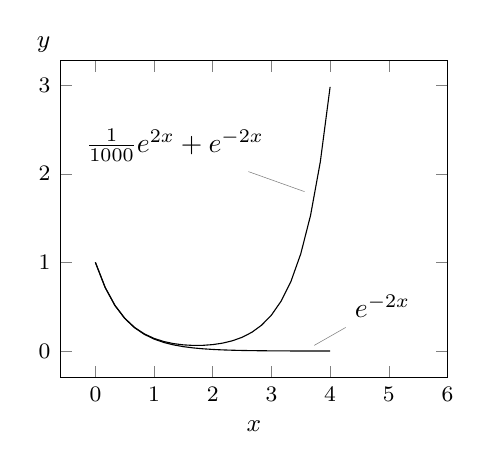
\begin{tikzpicture}
\begin{axis}[small,xmax=6,xlabel={$x$},ylabel={$y$},ylabel style={rotate=-90},ylabel style={at={(axis description cs:0,1.05)}}]
\addplot[domain=0:4]{e^(-2*x)}node[pos=0.9,pin=30:{$e^{-2x}$}]{};
\addplot[domain=0:4]{1/1000*e^(2*x)+e^(-2*x)}node[pos=0.8,pin=150:{$\frac{1}{1000}e^{2x}+e^{-2x}$}]{};
\end{axis}
\end{tikzpicture}
\caption{سوال \حوالہ{سوال_سادہ_دو_درجی_غیر_مستحکم_الف} کے منحنی حل۔}
\label{شکل_سوال_سادہ_دو_درجی_غیر_مستحکم_الف}
\end{figure}

جوابات:\عددی{y=e^{-2x}} اور \عددی{y=\tfrac{1}{1000}e^{2x}+e^{-2x}}؛ شکل \حوالہ{شکل_سوال_سادہ_دو_درجی_غیر_مستحکم_الف} میں دونوں حل دکھائے گئے ہیں۔آپ دیکھ سکتے ہیں کہ ابتدائی قیمتوں میں انتہائی کم فرق حل پر بہت زیادہ اثر ڈالتی ہیں۔یہ \اصطلاح{غیر مستحکم}\فرہنگ{غیر مستحکم!صورت}\حاشیہب{instability}\فرہنگ{instability}  صورت کو ظاہر کرتی ہے۔زلزلے\فرہنگ{زلزلہ}  میں غیر مستحکم عمارتیں\فرہنگ{عمارت} انہیں وجوہات پر ڈھیر ہوتی ہیں۔فضا میں ہوا کا دباو، درجہ حرارت اور نمی کی تناسب بھی غیر مستحکم صورت پیدا کرتے ہوئے  تباہ کن آندھیوں کا سبب بنتی ہیں۔
\انتہا{سوال}
%=========================
\ابتدا{سوال}
استمراری مساوات کے جذر \عددی{\lambda_1=-2} اور \عددی{\lambda_2=3} ہیں۔مساوات \حوالہ{مساوات_سادہ_دو_درجی_مستقل_عددی_سر_الف} حاصل کریں۔

جواب:\عددی{y''-y'-6y=0} 
\انتہا{سوال}
%========================
\ابتدا{سوال}
استمراری مساوات کے جذر \عددی{\lambda_1} اور \عددی{\lambda_2} ہیں۔مساوات \حوالہ{مساوات_سادہ_دو_درجی_مستقل_عددی_سر_الف} میں  \عددی{a} اور \عددی{b} حاصل کریں۔ یوں جذر جانتے ہوئے تفرقی مساوات حاصل کی جا سکتی ہے۔

جواب:\عددی{a=-\lambda_1-\lambda_2}، \عددی{b=\lambda_1 \lambda_2}
\انتہا{سوال}
%========================
\ابتدا{سوال}
تفرقی مساوات \عددی{y''+ky'=0} کو موجودہ طریقے سے حل کریں۔ اسی کو تخفیف درجہ کی ترکیب سے بھی حل  کریں۔دونوں جواب کیوں یکساں ہونا ضروری ہے۔

جواب:\عددی{y=c_1+c_2e^{-kx}}؛ یکتائیت۔ 
\انتہا{سوال}
%=======================
\ابتدا{سوال}
دوہرا جذر کو منفرد \عددی{\lambda_1} اور \عددی{\lambda_2} کی وہ صورت تصور کی جا سکتی ہے جب \عددی{\lambda_2 \to \lambda_1} ہو۔\عددی{\lambda_2=\lambda_1+\Delta \lambda} لیتے اور ایک حل \عددی{=e^{\lambda_1 x}} لیتے ہوئے اساس کا دوسرا رکن  \عددی{xe^{\lambda_1 x}} تلاش کریں۔

حل:دوسرا حل \عددی{e^{\lambda_2 x}=e^{(\lambda_1 +\Delta \lambda)x}=e^{\lambda_1 x}e^{\Delta \lambda x}} ہے۔\عددی{e^{\Delta \lambda x}} کا مکلارن تسلسل لیتے ہوئے \عددی{\Delta \lambda \to 0} کی بنا صرف پہلے دو ارکان لیتے ہیں۔
یوں  \عددی{e^{\Delta \lambda x}=1+\frac{\Delta \lambda x}{1!}+\frac{(\Delta \lambda x)^2}{2!}+\cdots \approx 1+\Delta \lambda x} ہو گا اور 
\عددی{e^{\lambda_2 x}=e^{\lambda_1 x}+\Delta \lambda xe^{\lambda_1 x}} لکھا جا سکتا ہے۔اب چونکہ \عددی{e^{\lambda_1 x}} پہلے سے اساس کا حصہ ہے لہٰذا اساس کا دوسرا رکن \عددی{xe^{\lambda_1 x}} ہو گا جہاں \عددی{\Delta \lambda} کو مستقل تصور کرتے ہوئے رد کیا جاتا ہے
\انتہا{سوال}

\حصہ{تفرقی عامل}
آپ \عددی{y=\sin x} یا \عددی{y=\tfrac{\dif f(x)}{\dif x}} کے عمل سے بخوبی واقف ہیں۔پہلی مثال میں کسی مقدار یا تفاعل \عددی{x} پر عامل \عددی{\sin} عمل کرتے ہوئے ایک نیا تفاعل دیتا ہے۔یوں \عددی{x=\tfrac{\pi}{2}} پر \عددی{\sin \tfrac{\pi}{2}=1} حاصل ہوتا ہے۔ ہم کہتے ہیں کہ \اصطلاح{عامل}\فرہنگ{عامل}\حاشیہب{operator}\فرہنگ{operator} \عددی{\sin} تفاعل \عددی{x} کے نقطہ \عددی{x=\tfrac{\pi}{2}} سے مبدل تفاعل \عددی{y} کا نقطہ \عددی{y=1} دیتا ہے۔اسی طرح \اصطلاح{عامل} \عددی{\tfrac{\dif}{\dif x}} تفاعل \عددی{x^3} پر عمل کرتے ہوئے تفاعل \عددی{3x^2} دیتا ہے۔

یہ بتلاتا چلوں کہ ریاضیات اور طبیعیات میں عامل کا استعمال نہایت اہم کردار ادا کرتا ہے۔ یہاں بالخصوص \اصطلاح{کوانٹم میکانیات}\فرہنگ{کوانٹم میکانیات}\حاشیہب{quantum mechanics}\فرہنگ{quantum mechanics} کا ذکر کرنا لازم جہاں عامل کا استعمال کثرت سے کیا جاتا ہے۔ 

اس کتاب میں ہم صرف \اصطلاح{تفرقی عامل}\فرہنگ{تفرقی!عامل}\فرہنگ{عامل!تفرقی}\حاشیہب{differential operator}\فرہنگ{operator!differential}\فرہنگ{differential!operator} \عددی{D} پر بحث کریں گے جہاں \عددی{D=\tfrac{\dif}{\dif x}} ہے۔ یوں ایک درجی تفرق
\begin{align}
Dy=y'=\frac{\dif y}{\dif x}
\end{align}
لکھا جائے گا۔اسی طرح دو درجی تفرق \عددی{D^2y=D(Dy)=y''} اور تین درجی تفرق \عددی{D^3 y=y'''} لکھا جائے گا۔اس طرح \عددی{D \sin x=\cos x} اور \عددی{D^2 \sin x=-\sin x} ہو گا۔

خطی متجانس مساوات \عددی{y''+ay'+by=0} جہاں \عددی{a} اور \عددی{b} مستقل مقدار ہیں میں \اصطلاح{دو درجی تفرقی عامل}
\begin{align*}
L=P(D)=D^2+aD+bI
\end{align*}
متعارف کرتے ہیں جہاں \عددی{I} \اصطلاح{مماثلی عامل}\فرہنگ{عامل!مماثلی}\فرہنگ{مماثلی!عامل}\حاشیہب{identity operator}\فرہنگ{operator!identity}\فرہنگ{identity!operator} ہے جس کی تعریف \عددی{Iy=y} ہے۔اس طرح دیے گئے تفرقی مساوات کو درج ذیل لکھا جا سکتا ہے۔
\begin{align}\label{مساوات_سادہ_دو_درجی_کثیر_رکنی_تفرقی_عامل_الف}
Ly=P(D)y=(D^2+aD+bI)y=0
\end{align}
\عددی{L} خطی عامل اور \عددی{P} کثیر رکنی\فرہنگ{کثیر رکنی}\حاشیہب{polynomial}\فرہنگ{polynomial} ہے۔یوں اگر \عددی{Lw} اور \عددی{Ly} پائے جاتے ہوں (یعنی \عددی{w} اور \عددی{y} دو مرتبہ قابل تفرق ہوں) تب \عددی{L(cy+kw)} بھی پایا جاتا ہے جہاں \عددی{c} اور \عددی{k} کوئی مستقل ہیں۔مزید درج ذیل لکھا جا سکتا ہے۔
\begin{align}
L(cy+kw)=cLy+kLw
\end{align}

چونکہ \عددی{De^{\lambda x}=\lambda e^{\lambda x}} اور \عددی{D^2 e^{\lambda x}=\lambda^2 e^{\lambda x}} ہیں لہٰذا 
\begin{gather}
\begin{aligned}
Le^{\lambda x}&=(D^2+aD+bI)e^{\lambda x}\\
&=(\lambda^2+a\lambda+b)e^{\lambda x}=P(\lambda) e^{\lambda x}=0
\end{aligned}
\end{gather}
ہو گا۔حصہ \حوالہ{حصہ_سادہ_دو_درجی_مستقل_عددی_سر} میں بھی ہم نے یہی نتیجہ اخذ کیا تھا کہ \عددی{e^{\lambda x}} صرف اور صرف اس صورت اس تفرقی مساوات کا حل ہو گا اگر \عددی{\lambda} امتیازی مساوات \عددی{P(\lambda)=0} کا جذر ہو۔

یہاں دلچسپ بات یہ ہے کہ \عددی{P(\lambda)} عام الجبرائی کثیر رکنی ہے جس کی تجزی\فرہنگ{تجزی}\حاشیہب{factorization}\فرہنگ{factorization} کی جا سکتی ہے۔\عددی{\lambda} کی جگہ \عددی{D} پر کرنے سے  \اصطلاح{کثیر رکنی عامل} حاصل ہوتا ہے۔
%================================

\ابتدا{مثال}\quad تفرقی مساوات کا حل بذریعہ تجزی\\
کثیر رکنی \عددی{P(D)=D^2+4D-21I} کی تجزی سے \عددی{P(D)=0} کو حل کریں۔

حل:\عددی{I^2=1} لیتے ہوئے \عددی{D^2+4D-21I=(D-3)(D+7)} لکھا جا سکتا ہے۔اب \عددی{(D-3)y=y'-3y=0} کا حل \عددی{y_1=e^{3x}} اور \عددی{()y=y'+7y=0} کا حل \عددی{y_2=e^{-7x}} ہے۔یہ جوابات کسی بھی وقفے پر حل کی اساس ہیں۔آئیں تفرقی مساوات حاصل کریں۔
\begin{align*}
(D-3)(D+7)y=(D-3)(y'+7y)=y''+7y'-3y'-21y=y''+4y'-21y=0
\end{align*}
\انتہا{مثال}
%===============================

مساوات \حوالہ{مساوات_سادہ_دو_درجی_کثیر_رکنی_تفرقی_عامل_الف} میں کثیر رکنی کے عددی سر مستقل مقدار ہیں۔ایسی صورت میں تفرقی عامل کے استعمال سے تفرقی مساوات حل کرنا نہایت آسان ثابت ہوتا ہے۔عددی سر مستقل نہ ہونے کی صورت میں تفرقی عامل کا استعمال نہایت پیچیدہ ثابت ہوتا ہے جس پر اس کتاب میں تبصرہ نہیں کیا جائے گا۔

%===================================
%===================================

\حصہء{سوالات}
سوال \حوالہ{سوال_سادہ_دو_درجی_تفرقی_عامل_الف} تا سوال \حوالہ{سوال_سادہ_دو_درجی_تفرقی_عامل_ب} دیے تفاعل پر دیا تفرقی عامل لاگو کریں۔
  
%===============
\ابتدا{سوال}\شناخت{سوال_سادہ_دو_درجی_تفرقی_عامل_الف}
\begin{align*}
D+2I; \quad x^3, \quad \cos 5x, \quad e^{-kx}, \quad \cosh x
\end{align*}
جوابات:\عددی{3x^2+2x^3}، \عددی{-5\sin 5x+2\cos 5x}، \عددی{(2-k)e^{-kx}}، \عددی{\sinh x+2\cosh x}
\انتہا{سوال}
%=======================
\ابتدا{سوال}
\begin{align*}
D^2-3D; \quad 2x^4-x, \quad 2\sinh 2x-\cos 5x
\end{align*}
جوابات:\عددی{24x^2-24x^3+3}، \عددی{-15\sin 5x-12\cosh 2x+25\cos 5x+\sinh 2x}
\انتہا{سوال}
%==================================
\ابتدا{سوال}
\begin{align*}
(D+2I)^2; \quad e^{3x}, \quad xe^{2x}
\end{align*}
جوابات:\عددی{25e^{3x}}، \عددی{(12x+8)e^{2x}}
\انتہا{سوال}
%==================================
\ابتدا{سوال}
\begin{align*}
(D-3I)^2; \quad e^{2x}, \quad xe^{3x}
\end{align*}
جوابات:\عددی{e^{2x}}، \عددی{0}
\انتہا{سوال}
%==================================
\ابتدا{سوال}\شناخت{سوال_سادہ_دو_درجی_تفرقی_عامل_ب}
\begin{align*}
(D+I)(D-2I); \quad e^{2x}, \quad xe^{2x}
\end{align*}
جوابات:\عددی{-2e^{2x}}، \عددی{2(1-x)e^{2x}}
\انتہا{سوال}
%==================================

سوال \حوالہ{سوال_سادہ_دو_درجی_تفرقی_عامل_پ} تا سوال \حوالہ{سوال_سادہ_دو_درجی_تفرقی_عامل_ت} کی تجزی حاصل کرتے ہوئے حل کریں۔

%==============================
\ابتدا{سوال}\شناخت{سوال_سادہ_دو_درجی_تفرقی_عامل_پ}
\begin{align*}
(D^2-9I)y=0
\end{align*}
جواب:\عددی{y=c_1e^{3x}+c_2e^{-3x}}
\انتہا{سوال}
%===========================
\ابتدا{سوال}
\begin{align*}
(D^2+4D+4I)y=0
\end{align*}
جواب:دوہرا جذر پایا جاتا ہے لہٰذا دوسرا حل \عددی{xe^{2x}} لیتے ہوئے \عددی{y=(c_1+c_2 x)e^{2x}} ملتا ہے۔
\انتہا{سوال}
%===========================
\ابتدا{سوال}
\begin{align*}
(D^2+4D+13I)y=0
\end{align*}
جواب:\عددی{y=e^{-2x}(c_1 \cos 3x+c_2 \sin 3x)}
\انتہا{سوال}
%===========================
\ابتدا{سوال}
\begin{align*}
(4D^2+4D-17I)y=0
\end{align*}
جواب:\عددی{y=e^{\tfrac{x}{2}}(c_1 \cos 2x+c_2 \sin 2x)}
\انتہا{سوال}
%===========================
\ابتدا{سوال}\شناخت{سوال_سادہ_دو_درجی_تفرقی_عامل_ت}
\begin{align*}
(9D^2+12D+4I)y=0
\end{align*}
جواب:دوہرا جذر پایا جاتا ہے۔ \عددی{y=(c_1+c_2 x)e^{-\tfrac{2}{3}x}}
\انتہا{سوال}
%===========================
%===========================

\حصہ{اسپرنگ سے جڑی کمیت کی آزادانہ ارتعاش}\شناخت{حصہ_سادہ_اسپرنگ_کمیت}
مستقل قیمت کے عددی سر والے خطی سادہ تفرقی مساوات  میکانی ارتعاش میں کلیدی کردار ادا کرتے ہیں۔اس حصے میں اسپرنگ سے جڑی کمیت کی حرکت پر غور کیا جائے گا۔اس نظام کو \اصطلاح{اسپرنگ اور کمیت}\فرہنگ{اسپرنگ!کمیت}\فرہنگ{کمیت!اسپرنگ}\فرہنگ{ارتعاش!اسپرنگ اور کمیت} کا نظام کہا جائے گا جسے شکل \حوالہ{شکل_سادہ_دو_درجی_اسپرنگ_کمیت_نظام} میں دکھایا گیا ہے۔
\begin{figure}
\centering
\begin{tikzpicture}
\node[circle,fill=gray,inner sep=2.5mm] (a) at (0,0) {};
\node[circle,fill=gray,inner sep=2.5mm] (b) at (3,2) {};
\node[circle,inner sep=2.5mm] (c) at (6,2.5) {};
\draw[decoration={aspect=0.3, segment length=3mm, amplitude=3mm,coil},decorate] (0,5) -- (a); 
\draw[decoration={aspect=0.3, segment length=1.7mm, amplitude=3mm,coil},decorate] (3,5) -- (b); 
\draw[decoration={aspect=0.3, segment length=1.5mm, amplitude=3mm,coil},decorate] (6,5) -- (c); 
\fill [pattern = north east lines] (-1,5) rectangle (7,5.2);
\draw[thick] (-1,5) -- (7,5);
%dashed lines
\draw  (c)++(0,0.37) node[below]{\RL{ڈھیلا اسپرنگ}};
\draw[dashed] (c)++(0.5,0.37)coordinate(cR)--++(-2.75,0)coordinate(cL);
\draw  (b)++(0,-0.37) node[below]{\RL{ساکن نظام}};
\draw[dashed] (b)++(1.5,0.37)coordinate(bR)--++(-3.75,0)coordinate(bL);
\draw  (a)++(0,-0.37) node[below]{\RL{ارتعاش پذیر نظام}};
\draw[dashed] (a)++(0,0.37)coordinate(aR)--++(2.3,0)coordinate(aL);
%dimensions
\draw[stealth-stealth] (cL)++(0.5,0)coordinate(cT)--($(bL)!(cT)!(bR)$)node[pos=0.5, right]{$s_0$};
\draw[-stealth] (bL)++(0.2,0)coordinate(bT)--($(aL)!(bT)!(aR)$)node[pos=0.5, right]{$y$};
\draw(b)++(-0.5,0.37)node[left,fill=white]{$(y=0)$};
\end{tikzpicture}
\caption{اسپرنگ اور کمیت کا غیر قصری نظام۔}
\label{شکل_سادہ_دو_درجی_اسپرنگ_کمیت_نظام}
\end{figure}

ایک عام اسپرنگ جو لمبائی میں اضافہ اور کمی کو روکتا ہو کو شکل \حوالہ{شکل_سادہ_دو_درجی_اسپرنگ_کمیت_نظام} میں مستحکم سلاخ سے لٹکایا ہوا دکھایا گیا ہے۔اس کی نچلی سر سے کمیت \عددی{m} کی لوہے کا گیند لٹکانے سے  اسپرنگ کی لمبائی میں  \عددی{s_0} اضافہ پیدا ہوتا ہے۔اس ساکن نظام میں اسپرنگ کے نچلے سر کو \عددی{y=0} تصور کیا جاتا ہے۔ہم نیچے رخ کو مثبت رخ تصور کرتے ہیں۔یوں نیچے رخ  قوت کو مثبت اور اوپر رخ  قوت کو منفی تصور کیا جائے گا۔اسی طرح مقام \عددی{y=0} سے نیچے رخ  فاصلہ \عددی{y} مثبت ہو گا۔مزید اسپرنگ کی کمیت کو گیند کی کمیت سے اتنا کم تصور کیا جاتا ہے کہ اسپرنگ کی کمیت کو درج ذیل تبصرے میں رد کیا جا سکتا ہے۔

ساکن حالت میں اسپرنگ پر نیچے رخ قوت \عددی{mg} عمل کرتا ہے جس سے  اسپرنگ  کی لمبائی میں \عددی{s_0} اضافہ پیدا ہوتا ہے۔ یہاں \عددی{g=\SI{9.8}{\meter\per\second\squared}} ثقلی اسراع اور \عددی{mg} گیند کا وزن ہے۔اسپرنگ کی لمبائی میں اضافے  کی وجہ سے، \اصطلاح{قانون ہک}\فرہنگ{قانون ہک}\فرہنگ{ہک کا قانون}\حاشیہب{Hooke's law}\فرہنگ{Hooke's law} کے تحت\حاشیہد{روبرٹ ہک (1635-1703) انگلستان  کے ماہر طبیعیات تھے۔}، اسپرنگ اوپر رخ  \اصطلاح{بحالی قوت}\فرہنگ{بحالی قوت}\فرہنگ{قوت!بحالی}\حاشیہب{restoring force}\فرہنگ{restoring force}\فرہنگ{force!restoring}  \عددی{F_0=-ks_0} پیدا کرتا ہے جہاں \عددی{k} \اصطلاح{اسپرنگ مستقلہ}\فرہنگ{اسپرنگ!مستقلہ}\فرہنگ{مستقل!اسپرنگ}\حاشیہب{spring constant}\فرہنگ{spring constant} ہے جس کو \عددی{\si{\kilo\gram\per\second\squared}} یعنی \عددی{\si{\newton\per\meter}} میں ناپا جاتا ہے۔بحالی قوت اسپرنگ کی لمبائی میں تبدیلی کو روکنے کی کوشش کرتا ہے۔قوت \عددی{mg} مثبت رخ ہے لہٰذا اس کو مثبت لکھا گیا ہے جبکہ قوت \عددی{-k s_0} منفی رخ ہے لہٰذا اس کو منفی لکھا گیا ہے۔ان قوتوں کا مجموعہ صفر \عددی{mg-ks_0=0} کے برابر ہوتا ہے۔اگر ان قوتوں کا مجموعہ صفر کے برابر نہ ہوتا تو گیند ساکن نہ ہوتا بلکہ نیوٹن کے قانون \عددی{ّF=my''} کے تحت حرکت کرتا۔طاقتور اسپرنگ کے مستقلہ \عددی{k} کی قیمت زیادہ ہوتی ہے۔ان دونوں قوتوں کی مقدار گیند کی حرکت سے تبدیل نہیں ہوتی لہٰذا ان کا مجموعہ ہر وقت صفر کے برابر ہو گا۔یوں گیند کی حرکت میں ان دونوں قوتوں کا کوئی کردار نہیں ہے لہٰذا ان پر مزید بات نہیں کی جائے گی۔

فرض کریں کہ گیند کو نیچے رخ کھینچ کر چھوڑا جاتا ہے۔شکل \حوالہ{شکل_سادہ_دو_درجی_اسپرنگ_کمیت_نظام} میں گیند کو ساکن مقام سے لمحاتی طور \عددی{y} فاصلے پر دکھایا گیا ہے۔اس لمحہ اسپرنگ اضافی بحالی قوت \عددی{F_1=-ky} پیدا کرتا ہے جس کے تحت گیند نیوٹن کے قانون
\begin{align}
F_1=ma = my''
\end{align}
 کے تحت حرکت کرے گا جہاں \عددی{y''=\tfrac{\dif^2 y}{\dif t^2}} ہے۔

\حصہء{بلا تقصیر حرکت کی سادہ تفرقی مساوات}
ہر نظام تقصیری ہوتا ہے ورنہ حرکت کبھی بھی نہ رکتی۔ نہایت کم تقصیری نظام  جس کے حرکت کا مطالعہ نسبتاً کم دورانیے کے لئے  کیا جائے میں تقصیر کو نظر انداز کیا جا سکتا ہے۔یوں اس کو بلا تقصیر تصور کیا جا سکتا ہے۔ شکل \حوالہ{شکل_سادہ_دو_درجی_اسپرنگ_کمیت_نظام} کا نظام بلا تقصیر نظام کی عمدہ مثال ہے۔نیوٹن کے قانون کو بروئے کار لیتے ہوئے اس نظام کی تفرقی مساوات لکھتے ہیں۔
\begin{align}
my''+ky=0
\end{align}
یہ مستقل عددی سر والا خطی متجانس سادہ تفرقی مساوات ہے جس کا امتیازی مساوات \عددی{\lambda^2+\tfrac{k}{m}=0} ہے۔امتیازی مساوات کے جوڑی دار مخلوط جذر \عددی{\lambda=\mp i \sqrt{\tfrac{k}{m}}=\mp i \omega_0} ہیں جن سے عمومی حل لکھتے ہیں۔
\begin{align}\label{مساوات_سادہ_دو_درجی_اسپرنگ_کمیت_ارتعاش_الف}
y=A \cos \omega_0 t+B \sin \omega_0 t \quad \quad \omega_0=\sqrt{\frac{k}{m}}
\end{align}
اس حرکت کو \اصطلاح{ہارمونی ارتعاش}\فرہنگ{ہارمونی ارتعاش}\حاشیہب{harmonic oscillation}\فرہنگ{harmonic oscillation} کہتے ہیں جس کی \اصطلاح{تعدد}\فرہنگ{تعدد}\حاشیہب{frequency}\فرہنگ{frequency}  \عددی{f_0=\frac{\omega_0}{2\pi}} \اصطلاح{ہرٹز}\فرہنگ{ہرٹز}\حاشیہب{Hertz}\فرہنگ{Hertz} ہے\حاشیہد{ہائنرک ہرٹز (1857-1894) جرمنی کے ماہر طبیعیات تھے جنہوں نے برقناطیسی امواج دریافت کئے۔}۔تعدد \عددی{f_0} کو نظام کی \اصطلاح{قدرتی تعدد}\فرہنگ{قدرتی تعدد}\فرہنگ{تعدد!قدرتی}\حاشیہب{natural frequency}\فرہنگ{natural frequency} کہتے ہیں۔چونکہ ایک سیکنڈ میں \عددی{f_0} چکر (پھیرے) پورے ہوتے ہیں لہٰذا ایک چکر \عددی{\tfrac{1}{f_0}} عرصے میں پورا ہو گا۔اس دورانیے کو \عددی{T} سے ظاہر کیا جاتا ہے اور اس کو \اصطلاح{دوری عرصہ}\فرہنگ{دوری عرصہ}\حاشیہب{time period}\فرہنگ{time period} کہتے ہیں۔
\begin{align}
T=\frac{1}{f_0}
\end{align}
\عددی{C=\sqrt{A^2+B^2}} اور \عددی{\delta=\tan^{-1} \tfrac{B}{A}} لیتے ہوئے مساوات \حوالہ{مساوات_سادہ_دو_درجی_اسپرنگ_کمیت_ارتعاش_الف} کو 
\begin{align}\label{مساوات_سادہ_دو_درجی_اسپرنگ_کمیت_ارتعاش_ب}
y=C\cos(\omega_0 t-\delta)
\end{align}
لکھا جا سکتا ہے جہاں \عددی{C} \اصطلاح{حیطہ}\فرہنگ{حیطہ}\حاشیہب{amplitude}\فرہنگ{amplitude} اور \عددی{\delta} \اصطلاح{زاویائی فرق}\فرہنگ{زاویائی فرق}\حاشیہب{phase angle}\فرہنگ{phase angle} کہلاتے ہیں۔  
\begin{figure}
\centering
\begin{tikzpicture}
\begin{axis}[small,axis lines*=middle,xlabel={$t$},ylabel={$y$},ylabel style={rotate=-90},xtick=\empty,ytick=\empty,xmin=0,ylabel style={at={(axis description cs:0,1.05)}},xlabel style={at={(axis description cs:1.05,0.475)}}]
\addplot[domain=0:360,samples=100]{cos(x)}node[pos=0.2,fill=white]{ب};
\addplot[domain=0:360,samples=100]{cos(x)+sin(x)}node[pos=0.3,fill=white]{الف};
\addplot[domain=0:360,samples=100]{cos(x)-sin(x)}node[pos=0.1,fill=white]{پ};
\end{axis}
\end{tikzpicture}
\caption{مساوات \حوالہ{مساوات_سادہ_دو_درجی_اسپرنگ_کمیت_ارتعاش_الف} کے عمومی اشکال۔}
\label{شکل_سادہ_دو_اسپرنگ_حرکت_الف}
\end{figure}

مساوات \حوالہ{مساوات_سادہ_دو_درجی_اسپرنگ_کمیت_ارتعاش_الف} (یعنی مساوات \حوالہ{مساوات_سادہ_دو_درجی_اسپرنگ_کمیت_ارتعاش_ب}) کو شکل \حوالہ{شکل_سادہ_دو_اسپرنگ_حرکت_الف} میں دکھایا گیا ہے۔دکھائے گئے تینوں منحنی میں ابتدائی فاصلہ \عددی{y(0)=A} ہے جبکہ ابتدائی رفتار \عددی{y'(0)=\omega_0 B} خط الف میں مثبت، ب میں صفر اور پ میں منفی ہے۔
%================================

\ابتدا{مثال}\شناخت{مثال_سادہ_دو_درجی_بلا_تقصیر_نظام}
ایک اسپرنگ سے \عددی{\SI{2}{\kilo\gram}} کمیت لٹکانے سے اسپرنگ کی لمبائی میں \عددی{\SI{61.25}{\centi\meter}} کا اضافہ پیدا ہوتا ہے۔اس اسپرنگ سے کتنی کمیت لٹکانے سے ایک ہرٹز \عددی{\SI{1}{\hertz}} کا ارتعاش حاصل کیا جا سکتا ہے؟ ساکن حالت سے کمیت کو \عددی{\SI{10}{\centi\meter}} نیچے کھینچ کر چھوڑا جاتا ہے۔ کمیت کی حرکت دریافت کریں۔

حل:قانون ہک کے تحت \عددی{mg=0.6125k} سے \عددی{k=\tfrac{2\times 9.8}{0.6125}=\SI{32}{\newton\per\meter}} حاصل ہوتا ہے۔ایک ہرٹز کی تعدد کے لئے \عددی{2\pi f_0=\sqrt{\tfrac{k}{m}}} سے \عددی{m=\tfrac{k}{(2\pi f_0)^2}=\tfrac{32}{(2\pi\times 1)^2}=\SI{0.811}{\kilo\gram}} حاصل ہوتا ہے۔

مساوات \حوالہ{مساوات_سادہ_دو_درجی_اسپرنگ_کمیت_ارتعاش_الف} میں \عددی{y(0)=\SI{0.10}{\meter}} اور \عددی{y'(0)=0} پر کرتے ہوئے \عددی{A=0.1} اور \عددی{B=0} حاصل ہوتا ہے لہٰذا حرکت کی مساوات \عددی{y=0.1\cos 2\pi t} ہو گی۔\عددی{y} کی قیمت میٹر میں ہو گی۔
\انتہا{مثال}
%==================================

\حصہء{قصری نظام کا سادہ تفرقی مساوات}\شناخت{حصہ_سادہ_دو_قصری_نظام}
شکل \حوالہ{شکل_سادہ_دو_درجی_اسپرنگ_کمیت_نظام_قصری} میں اسپرنگ اور کمیت کے نظام میں قوت روک \عددی{F_3=-cy'} کا اضافہ کیا گیا ہے جو ہر لمحہ حرکت کے الٹ رخ عمل کرتی ہے۔یوں \عددی{my''=-ky-cy'} لکھا جائے گا جس سے قصری نظام کی سادہ تفرقی مساوات 
\begin{align}\label{مساوات_سادہ_دو_درجی_قصری_نظام_الف}
my''+cy'+ky=0
\end{align}
حاصل ہوتی ہے۔گیند کے ساتھ چادر منسلک کی گئی ہے جو ایک طرف سے بند نلکی میں حرکت کرتے ہوئے توانائی کا ضیاع اور یوں قوت روک پیدا ہوتا ہے۔ اس حصے کو (توانائی کا) \اصطلاح{جاذب}\فرہنگ{جاذب}\حاشیہب{absorber}\فرہنگ{absorber} بھی کہا جاتا ہے۔اس سے قوت روک پیدا ہوتا ہے۔تجربے سے دیکھا گیا ہے کہ کم رفتار پر ایسی قوت رفتار کے راست تناسب ہوتی ہے۔ \عددی{c} \اصطلاح{قصری مستقل}\فرہنگ{قصری!مستقل}\فرہنگ{مستقل!قصری}\حاشیہب{damping constant}\فرہنگ{damping constant} کہلاتا ہے۔قصری مستقل از خود مثبت مستقل ہے۔یوں نیچے رخ رفتار، یعنی مثبت رفتار، کی صورت میں قصری قوت منفی، یعنی اوپر رخ، ہو گی۔
\begin{figure}
\centering
\begin{tikzpicture}
\pgfmathsetmacro{\width}{0.9}
\pgfmathsetmacro{\height}{0.9}
\node[circle,fill=gray,inner sep=2.5mm] (b) at (0,0) {} ++(-0.37,0)node[left]{گیند} ++(0.74,0) node[right]{$m$};
\draw[decorate,decoration={coil,aspect=0.3, segment length=1.7mm, amplitude=3mm}] (0,3) -- (b)node[pos=0.5,shift={(-0.8,0)}]{اسپرنگ}node[pos=0.5,shift={(0.6,0)}]{$k$}; 
\fill [pattern = north east lines] (-1,3) rectangle (1,3.2);
\draw[thick] (-1,3) -- (1,3);
%dashboard
\draw[] (b)--++(0,-0.8)coordinate(c);
\draw[ultra thick](c) ++(-\width/2+0.1,0)--++(\width-0.2,0);
\draw[thick] (c)++(-\width/2,\height/3)--++(0,-\height)--++(\width,0)--++(0,\height);
\draw(c)++(-\width/2,0)node[left]{\RL{روک (جاذب)}};
\draw(c)++(\width/2,0)node[right]{$c$};
\end{tikzpicture}
\caption{اسپرنگ اور کمیت کا قصری نظام۔}
\label{شکل_سادہ_دو_درجی_اسپرنگ_کمیت_نظام_قصری}
\end{figure}

قصری نظام کی مساوات خطی متجانس ہے جس سے  امتیازی مساوات (\عددی{m} سے تقسیم شدہ) لکھتے ہیں۔
\begin{align*}
\lambda^2+\frac{c}{m}\lambda+\frac{k}{m}=0
\end{align*}
اس دو درجی الجبرائی مساوات کے جذر لکھتے ہیں۔
\begin{align}\label{مساوات_سادہ_دو_درجی_تقصیری_مستقل}
\lambda_1=-\alpha+\beta, \quad \lambda_2=-\alpha-\beta \quad \text{جہاں} \quad \alpha=\frac{c}{2m}, \quad \beta=\frac{\sqrt{c^2-4mk}}{2m}
\end{align}
تقصیر کی مقدار پر \عددی{c^2-4mk} کی قیمت منحصر ہے جو تین مختلف صورتیں پیدا کرتی ہے۔
%===============================
 \begin{itemize}
\item[پہلی صورت:]
 \اصطلاح{زیادہ تقصیر}\فرہنگ{زیادہ تقصیر}\فرہنگ{تقصیر!زیادہ}\حاشیہب{over damping}\فرہنگ{over damping}\فرہنگ{damping!over} دو منفرد حقیقی جذر \quad $c^2>4mk$
\item[دوسری صورت:]
 \اصطلاح{فاصل تقصیر}\فرہنگ{فاصل تقصیر}\فرہنگ{تقصیر!فاصل}\حاشیہب{critical damping}\فرہنگ{critical damping}\فرہنگ{damping!critical} دوہرا حقیقی جذر \quad $c^2=4mk$
\item[تیسری صورت:]
 \اصطلاح{کم تقصیر}\فرہنگ{کم تقصیر}\فرہنگ{تقصیر!کم}\حاشیہب{under damping}\فرہنگ{under damping}\فرہنگ{damping!under} جوڑی دار مخلوط جذر \quad $c^2<4mk$ 
\end{itemize}
%==============================
اس قسم کی تین صورتیں ہم  صفحہ \حوالہصفحہ{لسٹ_سادہ_دو_درجی_تین_صورتیں_الف} پر پہلے دیکھ چکے ہیں۔

\حصہء{تین صورتوں کے حل}
\جزوحصہء{پہلی صورت}\quad زیادہ تقصیر\\
پہلی صورت میں قصری قوت اتنا زیادہ ہے کہ \عددی{c^2>4mk} ہے جس سے دو منفرد حقیقی جذر \عددی{\lambda_1} اور \عددی{\lambda_2} حاصل ہوتے ہیں۔ ایسی صورت میں مساوات \حوالہ{مساوات_سادہ_دو_درجی_قصری_نظام_الف} کا عمومی حل درج ذیل ہو گا۔
\begin{align}\label{مساوات_سادہ_دو_درجی_قصری_زیادہ_حل_الف}
y=c_1 e^{-(\alpha-\beta)t}+c_2e^{-(\alpha+\beta)t}
\end{align}
چونکہ \عددی{\alpha>0}، \عددی{\beta>0} اور \عددی{\beta^2=\alpha^2-\tfrac{k}{m}<\alpha^2} ہیں لہٰذا \عددی{\alpha-\beta} اور \عددی{\alpha+\beta} دونوں مثبت مقدار ہیں۔یوں  مساوات \حوالہ{مساوات_سادہ_دو_درجی_قصری_زیادہ_حل_الف} میں دونوں قوت نمائی تفاعل کی طاقت منفی ہو گی اور دونوں تفاعل کی قیمتیں نہایت تیزی سے گھٹے گی۔آپ دیکھ سکتے ہیں کہ \عددی{t \to \infty} پر \عددی{y(\infty) \to 0} ہو گا یعنی گیند ساکن ہو گا۔زیادہ قصری نظام میں قصری قوت اس تیزی سے نظام سے توانائی خارج کرتا ہے کہ نظام ارتعاش کرنے کے قابل نہیں رہتا۔

مساوات \حوالہ{مساوات_سادہ_دو_درجی_قصری_زیادہ_حل_الف} کو مختلف ابتدائی قیمتوں کے لئے شکل \حوالہ{شکل_سادہ_دو_درجی_تقصیری_حرکت_الف} میں دکھایا گیا ہے۔شکل-الف میں ابتدائی فاصلہ مثبت ہے جبکہ شکل-ب میں ابتدائی فاصلہ منفی ہے۔شکل-الف میں خط الف مثبت ابتدائی رفتار کے لئے کھینچا گیا ہے جبکہ خط ب صفر ابتدائی رفتار اور دو عدد خط پ کو منفی ابتدائی رفتار کے لئے کھینچا گیا ہے۔شکل-ب میں خط الف منفی ابتدائی رفتار کے لئے کھینچا گیا ہے جبکہ خط ب صفر ابتدائی رفتار اور دو عدد خط پ کو مثبت ابتدائی رفتار کے لئے کھینچا گیا ہے۔آپ دیکھ سکتے ہیں کہ زیادہ تقصیری نظام میں ارتعاش ممکن نہیں ہے اور نظام میں حرکت بہت جلد ختم ہو جاتی ہے۔
\begin{figure}
\centering
\begin{subfigure}{0.5\textwidth}
\centering
\begin{tikzpicture}
\pgfmathsetmacro{\al}{0.6}   %alpha
\pgfmathsetmacro{\be}{0.4}   %beta
\pgfmathsetmacro{\y}{1}   %initial distance POSITIVE
%
\pgfmathsetmacro{\v}{0.5}   %initial velocity  POSITIVE
\pgfmathsetmacro{\ca}{(\v+(\al+\be)*\y)/(2*\be)}
\pgfmathsetmacro{\cb}{\y-\ca}
%
\pgfmathsetmacro{\v}{0}   %initial velocity  ZERO
\pgfmathsetmacro{\cc}{(\v+(\al+\be)*\y)/(2*\be)}
\pgfmathsetmacro{\cd}{\y-\cc}
%
\pgfmathsetmacro{\v}{-0.5}   %initial velocity  NEGATIVE
\pgfmathsetmacro{\ce}{(\v+(\al+\be)*\y)/(2*\be)}
\pgfmathsetmacro{\cf}{\y-\ce}
%
\pgfmathsetmacro{\v}{-2}   %initial velocity  NEGATIVE
\pgfmathsetmacro{\cg}{(\v+(\al+\be)*\y)/(2*\be)}
\pgfmathsetmacro{\ch}{\y-\cg}
\begin{axis}[small,axis lines*=middle,xtick=\empty,ytick=\empty,xlabel={$t$},ylabel={$y$},xlabel style={at={(axis description cs:1.05,0.4)}},ylabel style ={rotate=-90},ylabel style={at={(axis description cs:0,1.05)}},xmin=0]
\addplot[domain=0:10,samples=50]{\ca*e^(-(\al-\be)*x)+\cb*e^(-(\al+\be)*x)}node[pos=0.3,fill=white]{الف};
\addplot[domain=0:10]{\cc*e^(-(\al-\be)*x)+\cd*e^(-(\al+\be)*x)}node[pos=0.3,fill=white]{ب};
\addplot[domain=0:10]{\ce*e^(-(\al-\be)*x)+\cf*e^(-(\al+\be)*x)}node[pos=0.3,fill=white]{پ};
\addplot[domain=0:10,samples=50]{\cg*e^(-(\al-\be)*x)+\ch*e^(-(\al+\be)*x)}node[pos=0.3,fill=white]{پ};
\end{axis}
\end{tikzpicture}
\caption*{(الف) ابتدائی فاصلہ مثبت ہے۔}
\end{subfigure}%
\begin{subfigure}{0.5\textwidth}
\centering
\begin{tikzpicture}
\pgfmathsetmacro{\al}{0.6}   %alpha
\pgfmathsetmacro{\be}{0.4}   %beta
\pgfmathsetmacro{\y}{-1}   %initial distance NEGATIVE
%
\pgfmathsetmacro{\v}{-0.5}   %initial velocity  NEGATIVE
\pgfmathsetmacro{\ca}{(\v+(\al+\be)*\y)/(2*\be)}
\pgfmathsetmacro{\cb}{\y-\ca}
%
\pgfmathsetmacro{\v}{0}   %initial velocity  ZERO
\pgfmathsetmacro{\cc}{(\v+(\al+\be)*\y)/(2*\be)}
\pgfmathsetmacro{\cd}{\y-\cc}
%
\pgfmathsetmacro{\v}{0.5}   %initial velocity POSITIVE
\pgfmathsetmacro{\ce}{(\v+(\al+\be)*\y)/(2*\be)}
\pgfmathsetmacro{\cf}{\y-\ce}
%
\pgfmathsetmacro{\v}{2}   %initial velocity POSITIVE
\pgfmathsetmacro{\cg}{(\v+(\al+\be)*\y)/(2*\be)}
\pgfmathsetmacro{\ch}{\y-\cg}
\begin{axis}[small,axis lines*=middle,xtick=\empty,ytick=\empty,xlabel={$t$},ylabel={$y$},xlabel style={at={(axis description cs:1.05,0.7)}},ylabel style ={rotate=-90},ylabel style={at={(axis description cs:0,1.05)}},xmin=0]
\addplot[domain=0:10,samples=50]{\ca*e^(-(\al-\be)*x)+\cb*e^(-(\al+\be)*x)}node[pos=0.3,fill=white]{الف};
\addplot[domain=0:10]{\cc*e^(-(\al-\be)*x)+\cd*e^(-(\al+\be)*x)}node[pos=0.3,fill=white]{ب};
\addplot[domain=0:10]{\ce*e^(-(\al-\be)*x)+\cf*e^(-(\al+\be)*x)}node[pos=0.3,fill=white]{پ};
\addplot[domain=0:10,samples=50]{\cg*e^(-(\al-\be)*x)+\ch*e^(-(\al+\be)*x)}node[pos=0.3,fill=white]{پ};
\end{axis}
\end{tikzpicture}
\caption*{(ب) ابتدائی فاصلہ منفی ہے۔}
\end{subfigure}%
\caption{تقصیری نظام میں حرکت بالمقابل وقت۔}
\label{شکل_سادہ_دو_درجی_تقصیری_حرکت_الف}
\end{figure}
%================================

\جزوحصہء{دوسری صورت}\quad فاصل تقصیر\\
زیادہ تقصیر اور کم تقصیر کے درمیان فاصل تقصیر کی صورت پائی جاتی ہے جہاں \عددیء{c^2=4mk} ہوتا ہے۔یوں \عددی{\beta=0} اور امتیازی مساوات کا دوہرا جذر \عددی{\lambda_1=\lambda_2=-\alpha} پایا جاتا ہے۔یوں مساوات \حوالہ{مساوات_سادہ_دو_درجی_قصری_نظام_الف} کا عمومی حل درج ذیل ہو گا۔
\begin{align}\label{مساوات_سادہ_دو_درجی_قصری_فاصل_حل_الف}
y=(c_1 +c_2 t)e^{-\alpha t}
\end{align}
یہ مساوات ساکن مقام \عددی{y=0} سے صرف ایک مرتبہ گزر سکتی ہے۔اس کو یوں سمجھا جا سکتا ہے کہ \عددی{e^{-\alpha t}} کبھی صفر یا منفی نہیں ہو سکتا جبکہ \عددی{c_1+c_2 t} صرف ایک صفر دیتا ہے۔اگر \عددی{c_1} اور \عددی{c_2} دونوں مثبت یا دونوں منفی ہوں تب  \عددی{c_1+c_2 t} کسی صورت  صفر نہیں ہو سکتا اور \عددی{y} صفر سے کبھی نہیں گزرے گا۔ 
\begin{figure}
\centering
\begin{tikzpicture}
\pgfmathsetmacro{\al}{0.6}   %alpha
\pgfmathsetmacro{\be}{0}   %beta
\pgfmathsetmacro{\y}{1}   %initial distance POSITIVE
%
\pgfmathsetmacro{\v}{0.5}   %initial velocity  POSITIVE
\pgfmathsetmacro{\ca}{\y}
\pgfmathsetmacro{\cb}{\v+\al*\ca}
%
\pgfmathsetmacro{\v}{0}   %initial velocity  ZERO
\pgfmathsetmacro{\cc}{\y}
\pgfmathsetmacro{\cd}{\v+\al*\cc}
%
\pgfmathsetmacro{\v}{-0.5}   %initial velocity  NEGATIVE
\pgfmathsetmacro{\ce}{\y}
\pgfmathsetmacro{\cf}{\v+\al*\ce}
%
\pgfmathsetmacro{\v}{-2}   %initial velocity  NEGATIVE
\pgfmathsetmacro{\cg}{\y}
\pgfmathsetmacro{\ch}{\v+\al*\cg}
\begin{axis}[small,axis lines*=middle,xtick=\empty,ytick=\empty,xlabel={$t$},ylabel={$y$},xlabel style={at={(axis description cs:1.05,0.4)}},ylabel style ={rotate=-90},ylabel style={at={(axis description cs:0,1.05)}},xmin=0]
\addplot[domain=0:10,samples=50]{(\ca+\cb*x)*e^(-\al*x)}node[pos=0.3,fill=white]{الف};
\addplot[domain=0:10]{(\cc+\cd*x)*e^(-\al*x)}node[pos=0.3,fill=white]{ب};
\addplot[domain=0:10]{(\ce+\cf*x)*e^(-\al*x)}node[pos=0.3,fill=white]{پ};
\addplot[domain=0:10,samples=50]{(\cg+\ch*x)*e^(-\al*x)}node[pos=0.3,fill=white]{پ};
\end{axis}
\end{tikzpicture}
\caption{فاصل تقصیری نظام میں حرکت بالمقابل وقت۔}
\label{شکل_سادہ_دو_درجی_فاصل_تقصیری_حرکت_الف}
\end{figure}

شکل \حوالہ{شکل_سادہ_دو_درجی_فاصل_تقصیری_حرکت_الف} میں مساوات \حوالہ{مساوات_سادہ_دو_درجی_قصری_فاصل_حل_الف} کو مختلف ابتدائی قیمتوں کے لئے دکھایا گیا ہے۔ابتدائی فاصلہ مثبت لیا گیا ہے، خط الف میں ابتدائی رفتار مثبت، خط ب میں صفر اور دو عدد خط پ میں ابتدائی رفتار منفی لی گئی ہے۔یہ خطوط  شکل \حوالہ{شکل_سادہ_دو_درجی_تقصیری_حرکت_الف}-الف سے مشابہت رکھتے ہیں۔ایسا ہونا بھی چاہیے کیونکہ موجودہ صورت منفرد حقیقی جذر کی وہ مخصوص صورت ہے جہاں دونوں جذر عین برابر ہوں۔  
%================================

\جزوحصہء{تیسری صورت}\quad کم تقصیر\\
یہ سب سے زیادہ دلچسپ صورت ہے جہاں تقصیری مستقل کی قیمت اتنی کم ہے کہ \عددی{c^2-4mk<0} حاصل ہوتا ہے۔یوں مساوات \حوالہ{مساوات_سادہ_دو_درجی_تقصیری_مستقل}  میں \عددی{\beta} خیالی عدد ہو گا۔
\begin{align}\label{مساوات_سادہ_دو_کم_قصری_تعدد}
\beta=\frac{\sqrt{4mk-c^2}}{2m}=\sqrt{\frac{k}{m}-\frac{c^2}{4m^2}}=i\omega \quad\quad  (\omega >0)
\end{align}
امتیازی مساوات کے جذر جوڑی دار مخلوط اعداد ہوں گے
\begin{align}
\lambda_1=-\alpha+i\omega, \quad \lambda_2=-\alpha-i\omega
\end{align} 
اور مساوات \حوالہ{مساوات_سادہ_دو_درجی_قصری_نظام_الف} کا عمومی حل درج ذیل ہو گا
\begin{align}\label{مساوات_سادہ_دو_کم_قصری_ارتعاش_الف}
y=e^{-\alpha t} (A \cos \omega t+B \sin \omega t)=C e^{-\alpha t}  \cos (\omega t-\delta)
\end{align}
جہاں \عددی{C=\sqrt{A^2+B^2}} اور \عددی{\delta =\tan^{-1}\tfrac{B}{A}} ہیں۔

یہ \اصطلاح{قصری ارتعاش}\فرہنگ{قصری!ارتعاش}\فرہنگ{ارتعاش!قصری}\حاشیہب{damped oscillations}\فرہنگ{damped!oscillations}\فرہنگ{oscillations!damped} کو ظاہر کرتی ہے جس کو شکل \حوالہ{شکل_سادہ_دو_درجی_فاصل_قصری_ارتعاش_الف} میں دکھایا گیا ہے۔اس منحنی کی چوٹیاں، نقطہ دار لکیر سے دکھائی گئیں، تفاعل \عددی{y=Ce^{-\alpha t}} اور \عددی{y=-Ce^{-\alpha t}} کے منحنی کو چھوتی ہے۔ارتعاش کی تعدد \عددی{\tfrac{\omega}{2\pi}} ہے جو قصری مستقل \عددی{c} کم کرنے سے بڑھتی ہے۔قصری مستقل کی قیمت صفر کرنے سے مساوات \حوالہ{مساوات_سادہ_دو_درجی_اسپرنگ_کمیت_ارتعاش_ب} کی ہارمونی ارتعاش حاصل ہوتی ہے جس کی قدرتی تعدد  \عددی{\omega_0=\sqrt{\tfrac{k}{m}}} ہو گی۔
\begin{figure}
\centering
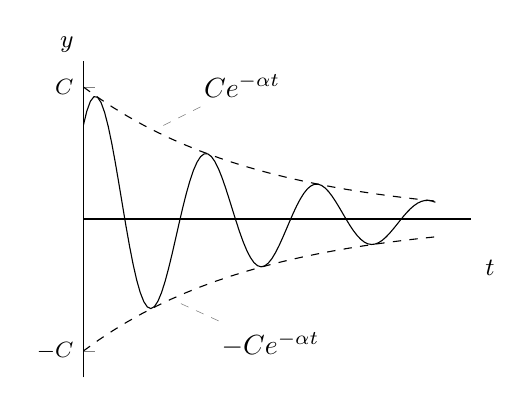
\begin{tikzpicture}
\begin{axis}[small,axis lines*=middle,xtick=\empty,ytick=\empty,xlabel={$t$},ylabel={$y$},xlabel style={at={(axis description cs:1.05,0.4)}},ylabel style ={rotate=-90},ylabel style={at={(axis description cs:0,1.05)}},xmin=0,ytick={1,0,-1},yticklabels={$C$,$0$,$-C$}]
\addplot[domain=0:20,samples=100]{e^(-0.1*x)*cos(x*180/pi-45)};
\addplot[dashed,domain=0:20]{e^(-0.1*x)}node[pos=0.2,pin=30:{$Ce^{-\alpha t}$}]{};
\addplot[dashed,domain=0:20]{-e^(-0.1*x)}node[pos=0.25,pin=-30:{$-Ce^{-\alpha t}$}]{};
\end{axis}
\end{tikzpicture}
\caption{قصری ارتعاش۔}
\label{شکل_سادہ_دو_درجی_فاصل_قصری_ارتعاش_الف}
\end{figure}
%=====================

\ابتدا{مثال}\شناخت{مثال_سادہ_دو_آزاد_حرکت}\quad تقصیری حرکت کے تین صورتیں\\
ایک اسپرنگ جس کا مستقل \عددی{k=\SI{32}{\newton\per\kilo\gram}} ہے سے \عددی{m=\SI{2}{\kilo\gram}} کا گیند لٹکایا گیا ہے۔اس نظام میں باری باری \عددی{c=\SI{20}{\kilo\gram\per\second}}، \عددی{c=\SI{16}{\kilo\gram\per\second}} اور \عددی{c=\SI{5}{\kilo\gram\per\second}} تقصیری اثر شامل  کیا جاتا ہے۔ابتدائی معلومات \عددی{y(0)=\SI{4}{\centi\meter}} اور \عددی{y'(0)=0} ہیں۔گیند کی حرکت دریافت کریں۔

حل:قوت روک نظام میں توانائی کے ضیاع کو ظاہر کرتی ہے جس سے مسلسل گھٹتی ارتعاش (پہلی صورت)  یا  غیر ارتعاشی حرکت (دوسری اور تیسری صورت) پیدا ہوتی ہے۔

پہلی صورت: \عددی{m=2}، \عددی{k=32} اور  \عددی{c=20} درج ذیل ابتدائی قیمت مسئلہ دیتی ہے
\begin{align*}
2y''+20y'+32y=0, \quad y(0)=\SI{0.04}{\meter}, \quad y'(0)=0
\end{align*}
جس کا امتیازی مساوات \عددی{2\lambda^2+20\lambda+32=0} ہے۔ امتیازی مساوات \عددی{2(\lambda+8)(\lambda+2)=0} کے جذر \عددی{\lambda_1=-2} اور \عددی{\lambda_2=-8} ہیں جن سے عمومی حل اور حل کا یک درجی تفرق لکھتے ہیں۔
\begin{align*}
y=c_1 e^{-2t}+c_2e^{-8t}, \quad y'=-2c_1e^{-2t}-8e^{-8t}
\end{align*}
ان میں ابتدائی قیمتیں پر کرتے ہوئے  \عددی{c_1+c_2=0.04} اور \عددی{-2c_1-8c_2=0} ملتا ہے جنہیں حل کرنے سے \عددی{c_1=\tfrac{4}{75}} اور 
\عددی{c_2=-\tfrac{1}{75}} حاصل ہوتا ہے۔اس طرح حرکت کی مساوات درج ذیل ہو گی۔
\begin{align*}
y=\frac{4}{75}e^{-2t}-\frac{1}{75}e^{-8t}
\end{align*}
یہ مسلسل گھٹتی ارتعاش ہے جو آخر کار \عددی{t\to \infty} پر \عددی{y \to 0} ہو گی یعنی بہت دیر بعد گیند ساکن ہو گا۔

دوسری صورت: \عددی{c=16} کی صورت میں امتیازی مساوات \عددی{2\lambda^2+16\lambda+32=0} یعنی \عددی{2(\lambda+4)^2=0} ہو گا جس کا دوہرا جذر \عددی{\lambda_1=\lambda_2=4} ہے۔یوں حرکت کی عمومی مساوات درج ذیل ہو گی
\begin{align*}
y=(c_1+c_2 x)e^{-4t}
\end{align*}  
جس میں ابتدائی معلومات پر کرتے ہوئے \عددی{c_1=0.04} اور \عددی{c_2=0.16} حاصل ہوتے ہیں جن سے مخصوص حل لکھتے ہیں۔
\begin{align*}
y=(0.04+0.16t)e^{-4t}
\end{align*}
تیسری صورت: تقصیری مستقل \عددی{c=\SI{5}{\kilo\gram\per\second}} لیتے ہوئے  تفرقی مساوات \عددی{2y''+5y'+32y=0} ہو گا جس سے امتیازی مساوات \عددی{2\lambda^2+5\lambda+32=0} حاصل ہوتی ہے۔امتیازی مساوات کے جوڑی دار مخلوط جذر \عددی{-1.25\mp 3.8i} ہیں جن سے عمومی مساوات اور عمومی مساوات کا تفرق لکھتے ہیں۔
\begin{align*}
y&=e^{-1.25t}\left(A\cos 3.8t+B\sin 3.8t\right)\\
y'&=-1.25e^{-1.25t}\left(A\cos 3.8t+B\sin 3.8t\right)+3.8e^{-1.25t}\left(-A\sin 3.8t+B\cos 3.8t\right)
\end{align*}
ابتدائی معلومات کو \عددی{y} کی مساوات میں پر کرنے  سے \عددی{A=0.04} حاصل ہوتا ہے جبکہ انہیں \عددی{y'} کی مساوات میں پر کرنے سے \عددی{-1.25A+3.8B=0} یعنی \عددی{B=-0.013} حاصل ہوتا ہے لہٰذا مخصوص حل درج ذیل ہو گا۔
\begin{align*}
y=e^{-1.25t} \left(0.04\cos 3.8t-0.013\sin 3.8t\right)
\end{align*}
آپ دیکھ سکتے ہیں کہ بلا تقصیری نظام کی قدرتی ارتعاش \عددی{\omega_0=\sqrt{\frac{32}{2}}=4} سے موجودہ تعدد \عددی{\omega=3.8} کم ہے۔شکل \حوالہ{شکل_سادہ_دو_درجی_آزاد_حرکت} میں اس مثال کی تینوں صورتوں کو دکھایا گیا ہے۔
%
\begin{figure}
\centering
\begin{tikzpicture}
\begin{axis}[small,axis lines*=middle,xlabel={$t$},ylabel={$y$},xlabel style={at={(axis description cs:1.05,0.4)}},ylabel style ={rotate=-90},ylabel style={at={(axis description cs:0,1.05)}},xmin=0,ytick={0.04,0,-0.04},yticklabels={$0.04$,$0$,$-0.04$},scaled y ticks=false]
\addplot[dashed,domain=0:4]{4/75*e^(-2*x)-1/75*e^(-8*x)};
\addplot[dashed,domain=0:4]{(0.04+0.16*x)*e^(-4*x)};
\addplot[domain=0:4,samples=100]{e^(-5/4*x)*(0.04*cos(3.8*180/pi*x)-0.013*sin(3.8*180/pi*x))};
\end{axis}
\end{tikzpicture}
\caption{مثال \حوالہ{مثال_سادہ_دو_آزاد_حرکت} کی آزاد حرکت کی تین صورتیں۔}
\label{شکل_سادہ_دو_درجی_آزاد_حرکت}
\end{figure}

\انتہا{مثال}
%====================================

اس حصے میں بیرونی قوتوں سے پاک  اسپرنگ اور کمیت کے نظام کی \اصطلاح{آزاد حرکت}\فرہنگ{آزاد!حرکت}\حاشیہب{free motion}\فرہنگ{free!motion} پر غور کیا گیا۔ایسے نظام کو \اصطلاح{متجانس} خطی سادہ تفرقی مساوات ظاہر کرتی ہے۔ہم اسی باب میں بیرونی جبری قوتوں کی موجودگی میں پائی جانے والی \اصطلاح{جبری حرکت}\حاشیہب{forced motion} پر بھی غور کریں گے۔ایسے نظام کو \اصطلاح{غیر متجانس} خطی سادہ تفرقی مساوات ظاہر کرتی ہے۔

%=============================
%===============================

\حصہء{سوالات}
سوال \حوالہ{سوال_سادہ_دو_خطی_متجانس_آزاد_حرکت_الف} تا سوال \حوالہ{سوال_سادہ_دو_خطی_متجانس_آزاد_حرکت_ب} بلا تقصیر، ہارمونی ارتعاش کے سوالات ہیں۔
%========================

\ابتدا{سوال}\شناخت{سوال_سادہ_دو_خطی_متجانس_آزاد_حرکت_الف} \quad ابتدائی قیمت مسئلہ\\
بلا تقصیر ارتعاش کو مساوات \حوالہ{مساوات_سادہ_دو_درجی_اسپرنگ_کمیت_ارتعاش_الف} ظاہر کرتی ہے۔ابتدائی فاصلہ \عددی{y(0)=y_0} اور ابتدائی رفتار \عددی{y'(0)=v_0} کی صورت میں مخصوص حل لکھیں۔

جواب: \عددی{y=y_0\cos \omega_0 t+\tfrac{v_0}{\omega_0}\sin \omega_0 t}
\انتہا{سوال}
%============================
\ابتدا{سوال}\quad تعدد\\
ایک اسپرنگ کی لمبائی \عددی{\SI{75}{\centi\meter}} ہے۔اس سے \عددی{\SI{0.25}{\kilo\gram}} کا گیند لٹکانے سے اسپرنگ کی لمبائی \عددی{\SI{85}{\centi\meter}} ہو جاتی ہے۔اس نظام کی تعدد \عددی{f_0} اور دوری عرصہ \عددی{T} کیا ہوں گے؟ 

جوابات:\عددی{f_0=\SI{1.58}{\hertz}}، \عددی{T=\SI{0.63}{\second}}
\انتہا{سوال}
%=========================
\ابتدا{سوال}\quad تعدد\\
اسپرنگ اور کمیت کی نظام میں کمیت چار گنّا کرنے سے تعدد پر کیا اثر پڑتا ہے۔مستقلہ اسپرنگ کی قیمت چار گنّا کرنے سے تعدد پر کیا اثر پڑتا ہے۔

 جوابات:کمیت چار گنّا کرنے سے تعدد آدھی ہوتی ہے۔مستقلہ اسپرنگ چار گنّا کرنے سے تعدد دگنی ہوتی ہے۔ 
\انتہا{سوال}
%=======================
\ابتدا{سوال}\quad ابتدائی رفتار\\
اسپرنگ اور کمیت کے نظام میں ابتدائی رفتار صفر نہ ہونے کی صورت میں نظام کے تعدد اور رفتار پر کیا اثر ہو گا؟

جواب:نظام کی تعدد پر کوئی اثر نہیں ہو گا البتہ اس سے رفتار بڑھے گی۔
\انتہا{سوال}
%=======================
\ابتدا{سوال}\شناخت{سوال_سادہ_دو_درجی_متوازی_اسپرنگ}\quad متوازی اسپرنگ\\
چار کلو گرام کی گیند کو \عددی{k_1=\SI{16}{\newton\per\meter}} کی اسپرنگ سے لٹکایا جاتا ہے۔نظام کی تعدد کیا ہو گی؟ اگر اسی گیند کو \عددی{k_2=\SI{32}{\newton\per\meter}} کی اسپرنگ سے لٹکایا جائے تب نظام کی تعدد کیا ہو گی؟ دونوں کی لمبائی برابر ہے۔  ان دونوں اسپرنگ کو متوازی جوڑا جاتا ہے۔ایسی صورت میں نظام کی تعدد کیا ہو گی؟ شکل \حوالہ{شکل_سوال_سادہ_دو_درجی_متوازی_اسپرنگ}-الف کو دیکھیے۔
\begin{figure}
\centering
\begin{subfigure}{0.5\textwidth}
\centering
\begin{tikzpicture}
\node[circle,fill=gray,inner sep=2.5mm] (b) at (0,0) {};
\draw[thick](b)--++(0,0.7)++(-1,0)coordinate(ka)--++(2,0)coordinate(kb);
\draw[decorate,decoration={coil,aspect=0.3, segment length=1.7mm, amplitude=3mm}] (-1,3) -- (ka); 
\node[circle,fill=gray,inner sep=2.5mm] (b) at (0,0) {};
\draw[decorate,decoration={coil,aspect=0.3, segment length=1.7mm, amplitude=3mm}] (1,3) -- (kb); 

\fill [pattern = north east lines] (-1.5,3) rectangle (1.5,3.2);
\draw[thick] (-1.5,3) -- (1.5,3);
\end{tikzpicture}
\caption*{(الف) سوال \حوالہ{سوال_سادہ_دو_درجی_متوازی_اسپرنگ} کا نظام۔}
\end{subfigure}%
\begin{subfigure}{0.5\textwidth}
\centering
\begin{tikzpicture}
\pgfmathsetmacro{\ang}{atan(1/3)}
\node[circle,fill=gray,inner sep=2.5mm] (b) at (1,0) {};
\draw[thick] (b)--(0,3)node[pos=0.6,right]{$L$};
\fill [pattern = north east lines] (-0.75,3) rectangle (0.75,3.2);
\draw[thick] (-0.75,3) -- (0.75,3);
\draw (b)++(0.37,0)node[right]{$m$};
\draw[dashed](0,3)--++(0,-2);
\draw[-stealth] ([shift={(-90:1.75)}]0,3) arc (-90:-90+\ang:1.75);
\draw(0,3)++(-90+\ang/2:2)node{$\theta$};
\end{tikzpicture}
\caption*{(ب) سوال \حوالہ{سوال_سادہ_دو_جھولا} کا نظام۔}
\end{subfigure}%
\caption{متوازی اسپرنگ اور جھولا  کے سوالات۔}
\label{شکل_سوال_سادہ_دو_درجی_متوازی_اسپرنگ}
\end{figure}

 جوابات:\عددی{\SI{0.32}{\hertz}}، \عددی{\SI{0.45}{\hertz}}، \عددی{\tfrac{1}{2\pi}\sqrt{\tfrac{k_1+k_2}{m}}=\SI{0.55}{\hertz}}
\انتہا{سوال}
%======================
\ابتدا{سوال}\quad سلسلہ وار اسپرنگ\\
گزشتہ سوال کے دونوں اسپرنگ کو سلسلہ وار جوڑا جاتا ہے۔نظام کی تفرقی مساوات لکھتے ہوئے تعدد حاصل کریں۔

جوابات:\عددی{my''+\tfrac{k_1 k_2}{k_1+k_2}y=0}، \عددی{f_0=\tfrac{1}{2\pi}\sqrt{\tfrac{k_1k_2}{(k_1+k_2)m}}=\SI{0.26}{\hertz}}
\انتہا{سوال}
%=========================
\ابتدا{سوال}\شناخت{سوال_سادہ_دو_جھولا}\quad جھولا\\
ایک ہلکے دھاگے سے \عددی{m} کمیت کا گیند لٹکایا شکل  \حوالہ{شکل_سوال_سادہ_دو_درجی_متوازی_اسپرنگ}-ب میں دکھایا گیا ہے۔اس نظام کی تفرقی مساوات حاصل کریں۔نہایت چھوٹے زاویے کی صورت میں \عددی{\sin \theta \approx \theta} لکھتے ہوئے مساوات کی سادہ صورت حاصل کریں جس کو حل کرتے ہوئے نظام کی تعدد حاصل کریں۔

حل:گیند کا وزن \عددی{mg} ہے جو نیچے رخ قوت ہے۔اس کا مماس \عددی{mg\sin \theta} ہے جو اسراع پیدا کرتا ہے۔ \عددی{L\theta''=g\sin \theta}، \عددی{L\theta''=g\theta}، \عددی{\theta=\cos \sqrt{\tfrac{g}{L}} t}، 
\عددی{f_0=\tfrac{1}{2\pi}\sqrt{\tfrac{g}{L}}}
\انتہا{سوال}
%=========================
\ابتدا{سوال}\شناخت{سوال_سادہ_دو_آرشمیدی}\quad اصول آرشمیدس\\
\اصطلاح{اصول آرشمیدس}\فرہنگ{آرشمیدس!اصول}\فرہنگ{اصول!آرشمیدس}\حاشیہب{Archimedian principle}\فرہنگ{Archimedese!principle} کے تحت جب کسی جسم کو مائع میں ڈبویا جائے تو اس پر قوت اچھال عمل کرتی ہے جس کی مقدار، جسم کے ڈبویے گئے حجم کے برابر، مائع کے وزن جتنی ہوتی ہے۔

ایک بیلن کو سیدھا  پانی میں کھڑا کرنے سے اس کا کچھ حصہ پانی میں ڈوب جاتا ہے۔شکل \حوالہ{شکل_سوال_سادہ_دو_آرشمیدی} میں اس کو ساکن حالت میں دکھایا گیا ہے۔بیلن کا
 رداس \عددی{r=\SI{20}{\centi\meter}} ہے۔اگر بیلن کو نیچے دھکیل کر چھوڑا جائے تو یہ دو سیکنڈ کے دوری عرصے سے اوپر نیچے ارتعاشی حرکت کرتا ہے۔بیلن کی کمیت \عددی{M} دریافت کریں۔ پانی کی کثافت \عددی{\rho=\SI{1000}{\kilo\gram\per\meter^3}} ہے۔ 
\begin{figure}
\centering
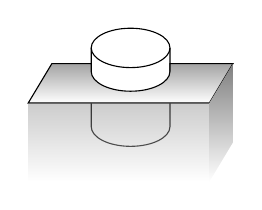
\begin{tikzpicture}
\pgfmathsetmacro{\ra}{0.5}
\pgfmathsetmacro{\rb}{0.25}
\pgfmathsetmacro{\h}{1}
\pgfmathsetmacro{\dX}{0.3}   %sheet sides
\pgfmathsetmacro{\kX}{0.5}
\pgfmathsetmacro{\kY}{0.5}
%cylinder
\draw([shift={(-180:\ra cm and \rb cm)}]0,0) arc (-180:180: \ra cm and \rb cm);
\draw(-180:\ra cm)--++(0,-\h cm) arc (-180:0:\ra cm and \rb cm)--++(0,\h cm);
%water surface
\draw[shade](-180:\ra cm)++(0,-0.2)--++(-\kX,0)--++(-\dX,-\kY)coordinate(kL)--++(\kX+\dX+2*\ra+\kX,0)coordinate(kR)--++(\dX,\kY)coordinate(kRB)--++(-\dX-\kX,0)--++(0,-0.1) arc (0:-180:\ra cm and \rb cm) --cycle;
\shade[opacity=0.4](kL)--++(0,-2*\kY)--++(\kX+\dX+2*\ra+\kX,0)coordinate(kRLow)--(kR)--cycle;
\shade(kRLow)--++(\dX,\kY)--++(0,2*\kY)--++(-\dX,-\kY)--cycle;
\end{tikzpicture}
\caption{آرشمیدسی اصول؛ سوال \حوالہ{سوال_سادہ_دو_آرشمیدی}}
\label{شکل_سوال_سادہ_دو_آرشمیدی}
\end{figure}

جوابات:\عددی{M=g\rho \pi r^2 \left(\tfrac{T}{2\pi}\right)^2=9.8\times 1000 \pi 0.2^2\left(\tfrac{2}{2\pi}\right)^2=\SI{124.8}{\kilo\gram}}
\انتہا{سوال}
%=======================
\ابتدا{سوال}\quad زنجیر کا میز سے پھسلنا\\
ایک پھسلنی میز پر زنجیر سیدھا پڑا ہوا ہے۔ ان کے مابین قوت رگڑ قابل نظر انداز ہے۔اگر زنجیر کے ایک سر کو میز سے لٹکایا جائے تو پورا زنجیر پھسلتے  پھسلتے نیچے گِر پڑتا ہے۔زنجیر کی کل لمبائی \عددی{L} اور کمیت \عددی{m} کلوگرام فی میٹر لیتے ہوئے اس مسئلے کا تفرقی مساوات لکھیں۔اگر \عددی{y(0)=0} اور \عددی{y'(0)=v_0} ہو تب مخصوص حل کیا ہو گا؟

جوابات:\عددی{mLy''=mgy}، \عددی{y=\tfrac{v_0}{2}\sqrt{\tfrac{L}{g}} \left(e^{\sqrt{\tfrac{g}{L}}t}-e^{-\sqrt{\tfrac{g}{L}}t}\right)}
\انتہا{سوال}
%=======================
\ابتدا{سوال}\شناخت{سوال_سادہ_دو_نالی_میں_پانی}\quad نالی میں پانی کی ارتعاش\\
شکل \حوالہ{شکل_سوال_سادہ_دو_نالی_میں_پانی}-الف میں \عددی{M=\SI{9}{\kilo\gram}} پانی زیر ثقلی قوت نالی میں ارتعاش کرتا ہے۔نالی کا اندرونی رداس \عددی{r=\SI{1.5}{\centi\meter}} ہے۔ ارتعاش کا دوری عرصہ  دریافت کریں۔ 
\begin{figure}
\centering
\begin{subfigure}{0.5\textwidth}
\centering
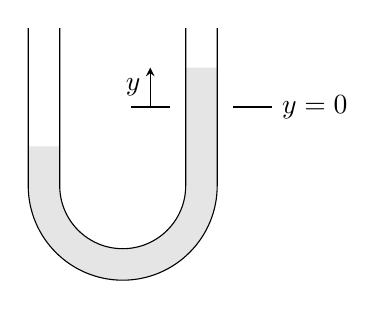
\begin{tikzpicture}
\pgfmathsetmacro{\d}{0.4}
\pgfmathsetmacro{\ra}{0.8}
\pgfmathsetmacro{\rb}{\ra+\d}
\pgfmathsetmacro{\h}{2}
%water
\fill[gray!20] (-\ra,\h/4)--++(0,-\h/4) arc (-180:0:\ra)--++(0,3/4*\h)--++(\d,0)--++(0,-3/4*\h) arc (0:-180:\rb)--++(0,\h/4)--cycle;
%pipe
\draw(-\ra,\h)--++(0,-\h) arc (-180:0:\ra)--++(0,\h);
\draw(-\rb,\h)--++(0,-\h) arc (-180:0:\rb)--++(0,\h);
%text
\draw (\ra-0.2,\h/2)--++(-0.5,0)coordinate[pos=0.5](ka);
\draw[-stealth](ka)--++(0,\h/4)node[pos=0.5,left]{$y$};
\draw (\rb+0.2,\h/2)--++(0.5,0)node[right]{$y=0$};
\end{tikzpicture}
\caption*{(الف) نالی میں پانی کا ارتعاش۔}
\end{subfigure}%
\begin{subfigure}{0.5\textwidth}
\centering
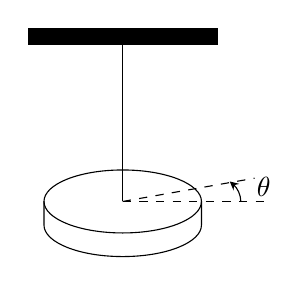
\begin{tikzpicture}
\draw(0,0) circle (1cm and 0.4 cm);
\draw(-1cm,0)--++(0,-0.3) arc (-180:0:1cm and 0.4cm)--++(0,0.3);
\draw(0,0)--++(0,2);
\draw[fill](-1.2,2) rectangle (1.2,2.2);
\draw[dashed] (0,0)--++(1.8cm,0);
\draw[dashed] (0,0)--++(10:1.7cm);
\draw[-stealth] ([shift={(0:1.5cm and 0.6cm)}]0,0) arc (0:25:1.5cm and 0.6cm);
\draw(6:1.8cm)node{$\theta$};
\end{tikzpicture}
\caption*{(ب)مروڑی ارتعاش۔}
\end{subfigure}%
\caption{سوال \حوالہ{سوال_سادہ_دو_نالی_میں_پانی} اور سوال \حوالہ{سوال_سادہ_دو_خطی_متجانس_آزاد_حرکت_ب} کے اشکال۔}
\label{شکل_سوال_سادہ_دو_نالی_میں_پانی}
\end{figure}

جوابات:\عددی{My''=-2\pi r^2 \rho g y}، \عددی{T=\SI{5.06}{\second}}
\انتہا{سوال}
%=====================
\ابتدا{سوال}\شناخت{سوال_سادہ_دو_خطی_متجانس_آزاد_حرکت_ب}
باریک غیر لچکدار تار سے  \عددی{I_0} \اصطلاح{جمودی معیار اثر}\فرہنگ{معیار اثر!جمودی}\فرہنگ{جمودی معیار اثر}\حاشیہب{moment of inertia}\فرہنگ{moment of inertia} کی ٹکی لٹکائی جاتی ہے جو مروڑی ارتعاش کرتی ہے۔شکل \حوالہ{شکل_سوال_سادہ_دو_نالی_میں_پانی}-ب کو دیکھیے۔اس نظام کو \عددی{I_0 \theta''+k\theta=0} تفرقی مساوات ظاہر کرتی ہے جہاں \عددی{\theta} کو  متوازن حال سے ناپا جاتا ہے۔ \عددی{k} مروڑی مستقل (یا اسپرنگ مستقلہ) ہے جس کو \عددی{\si{\newton\meter\per\radian}} نیوٹن میٹر فی ریڈیئن میں ناپا جاتا ہے۔ ابتدائی زاویہ \عددی{\theta_0=\tfrac{\pi}{4}} ریڈیئن یعنی \عددی{45^{\circ}} اور ابتدائی رفتار صفر ہے۔اس مساوات کو \عددی{\tfrac{k}{I_0}=\SI{9}{\per\second\squared}} لیتے ہوئے  حل کریں۔تعدد کا کلیہ دریافت کریں۔اس تجربے کو باریک تار کی مروڑی مستقل \عددی{k} حاصل کرنے کے لئے استعمال کیا جا سکتا  ہے۔ٹکی کا جمودی معیار اثر جانتے ہوئے اور قدرتی تعدد ناپ کر باریک تار کا مروڑی مستقل  دریافت کیا جا سکتا ہے۔ 

جواب:\عددی{\theta=\tfrac{\pi}{4}\cos 3t}، \عددی{f_0=\tfrac{1}{2\pi}\sqrt{\tfrac{k}{I_0}}}
\انتہا{سوال}
%=====================

سوالات \حوالہ{سوال_سادہ_دو_خطی_متجانس_آزاد_حرکت_پ} تا سوال \حوالہ{سوال_سادہ_دو_خطی_متجانس_آزاد_حرکت_پ} میں قصری حرکت پایا جاتا ہے۔

\ابتدا{سوال}\شناخت{سوال_سادہ_دو_خطی_متجانس_آزاد_حرکت_پ}\quad زیادہ تقصیر\\
زیادہ تقصیری صورت میں مساوات \حوالہ{مساوات_سادہ_دو_درجی_قصری_زیادہ_حل_الف} حل دیتی ہے۔ابتدائی معلومات \عددی{y(0)=y_0} اور \عددی{y'(0)=v_0} ہونے کی صورت میں \عددی{c_1} اور \عددی{c_2} دریافت کریں۔

جوابات:\عددی{c_1=\tfrac{1}{2}[(1+\tfrac{\alpha}{\beta})y_0+\tfrac{v_0}{\beta}]}،
 \عددی{c_2=\tfrac{1}{2}[(1-\tfrac{\alpha}{\beta})y_0-\tfrac{v_0}{\beta}]}
\انتہا{سوال}
%======================================
\ابتدا{سوال}\quad زیادہ تقصیر\\
زیادہ تقصیری صورت میں ثابت کریں کہ \عددی{y} زیادہ سے زیادہ ایک مرتبہ \عددی{y=0} سے گزر سکتا ہے۔

\انتہا{سوال}
%============================
\ابتدا{سوال}\quad دھچکا روک\\
گاڑیوں میں \اصطلاح{دھچکا روک}\فرہنگ{دھچکا روک}\فرہنگ{روک!دھچکا}\حاشیہب{shock absorber}\فرہنگ{shock absorber} نسب ہوتے ہیں جو گاڑی کی حرکت کو یقینی طور پر غیر ارتعاشی رکھتے ہیں۔صفحہ \حوالہصفحہ{شکل_سادہ_دو_درجی_اسپرنگ_کمیت_نظام_قصری} پر شکل \حوالہ{شکل_سادہ_دو_درجی_اسپرنگ_کمیت_نظام_قصری} دھچکا روک کو ظاہر کرتی ہے۔سوار کو دھچکوں سے پاک سواری اسپرنگ مہیا کرتا ہے جبکہ جاذب ان دھچکوں کی توانائی کو جذب کرتا ہے۔گاڑی بمع سواری کی کمیت کو \عددی{m} ظاہر کرتی ہے۔

کمیت \عددی{\SI{1300}{\kilo\gram}} اور اسپرنگ مستقل \عددی{\SI{80000}{\kilo\gram\per\second\squared}} ہونے کی صورت میں تقصیری مستقل کی وہ قیمت دریافت کریں جس پر یقین طور غیر ارتعاشی سواری حاصل ہو گی۔

  جواب:\عددی{c\ge \SI{20396}{\kilo\gram\per\second}}
\انتہا{سوال}
%============================
\ابتدا{سوال}\quad تعدد\\
کم قصری صورت کی ارتعاش کا تعدد \عددی{\omega}  مساوات \حوالہ{مساوات_سادہ_دو_کم_قصری_تعدد} دیتا ہے۔اس مساوات پر مسئلہ ثنائی کا اطلاق کرتے ہوئے پہلے دو اجزاء لیں اور  مثال \حوالہ{مثال_سادہ_دو_آزاد_حرکت} کی کم قصری حرکت \عددی{(c=\SI{5}{\kilo\gram\per\second})} کی تعدد ارتعاش حاصل کریں۔موجودہ جواب اور مثال میں حاصل کردہ جوابات میں کتنے فی صد فرق پایا جاتا ہے۔

جوابات:\عددی{\omega=\omega_0(1-\tfrac{c^2}{8mk})}، \عددی{\omega=3.8046} لہٰذا دونوں جوابات میں \عددی{\SI{0.13}{\percent}} فرق پایا جاتا ہے۔(مثال \حوالہ{مثال_سادہ_دو_آزاد_حرکت} میں تعدد کی بالکل ٹھیک قیمت \عددی{\omega=3.79967} ہے جسے مثال میں \عددی{\omega=3.8} لکھا گیا ہے۔)
\انتہا{سوال}
%==================================
\ابتدا{سوال}
بلا تقصیر نظام کے قدرتی تعدد اور کم تقصیری نظام (\عددی{\SI{5}{\kilo\gram\per\second}}) کے تعدد ارتعاش میں فرق مثال \حوالہ{مثال_سادہ_دو_آزاد_حرکت} کے لئے حاصل کریں۔

جواب:\عددی{\SI{4.88}{\percent}}؛ آپ دیکھ سکتے ہیں کہ اگرچہ قوت روک تعدد ارتعاش پر فرق ڈالتا ہے لیکن یہ فرق بہت زیادہ نہیں ہوتا۔
\انتہا{سوال}
%===================================
\ابتدا{سوال}
کم قصری ارتعاش کی مثبت چوٹیاں یکساں وقفوں پر پائی جاتی ہیں۔اس وقفے کو دریافت کریں۔ 

جواب:مساوات \حوالہ{مساوات_سادہ_دو_کم_قصری_ارتعاش_الف} کی مثبت چوٹیاں \عددی{\omega t-\delta=2n\pi} پر پائی جاتی ہیں جہاں \عددی{n=0,1,2\cdots} ہے۔یوں دو چوٹیوں کے درمیان وقفہ \عددی{\tfrac{2\pi}{\omega}} یعنی \عددی{T=\tfrac{1}{f}} ہو گا۔
\انتہا{سوال}
%==================================
\ابتدا{سوال}\quad لوگارتھمی گھٹاو\\
کم قصری نظام میں  دو قریبی چوٹیوں کی قیمتوں کی شرح ایک مستقل قیمت ہوتی ہے جس کے لوگارتھم کو \اصطلاح{لوگارتھمی گھٹاو}\فرہنگ{لوگارتھمی گھٹاو}\فرہنگ{گھٹاو!لوگارتھمی}\حاشیہب{logarithmic decrement}\فرہنگ{logarithmic decrement} کہتے ہیں۔لوگارتھمی گھٹاو \عددی{\Delta} حاصل کریں۔ 

جواب:\عددی{\Delta=\alpha T=\tfrac{2\pi \alpha}{\omega}}
\انتہا{سوال}
%========================
\ابتدا{سوال}\quad تقصیری مستقل\\
ایک کم تقصیری نظام میں \عددی{m=\SI{0.25}{\kilo\gram}} ہے اور ارتعاش کا دوری عرصہ \عددی{\SI{5}{\second}} ہے۔بیس چکروں میں چوٹی گھٹ کر \عددی{\tfrac{1}{4}} گنّا رہ جاتی ہے۔نظام کے تقصیری مستقل کا تخمینہ لگائیں۔

جواب:\عددی{\alpha=0.01386}
\انتہا{سوال}
%=========================
%==========================

\حصہ{یولر کوشی مساوات}
سادہ تفرقی مساوات\حاشیہد{لیون آرڈ یولر (1707-1783) سوئزرلینڈ کا رہائشی اور ماہر حساب تھا۔آگستن لوئی کوشی (1789-1857) فرانسیسی ماہر حساب تھا جنہوں نے جدید تجزیے کی بنیاد ڈالی۔} 
\begin{align}\label{مساوات_سادہ_دو_درجی_یولر_کوشی_الف}
x^2y''+axy'+by=0
\end{align}
\اصطلاح{یولر کوشی مساوات}\فرہنگ{یولر کوشی مساوات}\حاشیہب{Euler-Cauchy equation}\فرہنگ{Euler-Cauchy equation} کہلاتا ہے جہاں \عددی{a} اور \عددی{b} مستقل ہیں۔اس میں
\begin{align*}
y=x^m, \quad y'=mx^{m-1}, \quad y''=m(m-1)x^{m-2}
\end{align*}
پر کرنے سے
\begin{align*}
x^2m(m-1)x^{m-2}+axmx^{m-1}+bx^m=0
\end{align*}
ملتا ہے جس کو مشترک جزو \عددی{x^m} سے تقسیم کرتے ہوئے \اصطلاح{ذیلی مساوات}\فرہنگ{ذیلی مساوات}\حاشیہب{auxiliary equation}\فرہنگ{auxiliary equation} \عددی{m(m-1)+am+b=0} یعنی
\begin{align}\label{مساوات_سادہ_دو_درجی_یولر_کوشی_ب}
m^2+(a-1)m+b=0
\end{align}
حاصل ہوتی ہے۔یوں \عددی{y=x^m} مساوات \حوالہ{مساوات_سادہ_دو_درجی_یولر_کوشی_الف} کا حل اس صورت ہو گا جب \عددی{m} مساوات \حوالہ{مساوات_سادہ_دو_درجی_یولر_کوشی_ب} کا جذر ہو۔مساوات \حوالہ{مساوات_سادہ_دو_درجی_یولر_کوشی_ب} کے جذر
\begin{gather}
\begin{aligned}\label{مساوات_سادہ_دو_درجی_یولر_کوشی_پ}
m_1=\frac{1}{2}(1-a)+\sqrt{\frac{1}{4}(1-a)^2-b}, \quad m_2=\frac{1}{2}(1-a)-\sqrt{\frac{1}{4}(1-a)^2-b}
\end{aligned}
\end{gather}
ہیں۔

پہلی صورت: منفرد حقیقی جذر کی صورت میں دو منفرد حل 
\begin{align*}
y_1=x^{m_1},\quad y_2=x^{m_2}
\end{align*}
ملتے ہیں۔چونکہ ان حل کا حاصل تقسیم مستقل مقدار نہیں ہے لہٰذا یہ حل خطی طور غیر تابع ہیں۔اس طرح یہ حل کی اساس ہیں اور انہیں استعمال کرتے ہوئے عمومی حل
\begin{align}
y=c_1x^{m_1}+c_2x^{m_2}
\end{align}
لکھا جا سکتا ہے جہاں \عددی{c_1} اور \عددی{c_2} اختیاری مستقل ہیں۔یہ حل تمام \عددی{x} کے لئے درست ہے۔
%======================

\ابتدا{مثال}
یولر کوشی مساوات \عددی{x^2y''+0.5xy'-1.5y=0} سے \عددی{m^2-0.5m-1.5m=0} ذیلی مساوات حاصل ہوتی ہے جس کے جذر \عددی{m_1=1.5} اور \عددی{m_2=-1} ہیں۔ان سے اساس \عددی{y_1=x^{\tfrac{3}{2}}}، \عددی{y_2=x^{-1}} لکھی جا سکتی ہے۔اساس سے عمومی حل لکھتے ہیں۔
\begin{align*}
y=c_1x\sqrt{x}+\frac{c_2}{x}
\end{align*}
\انتہا{مثال}
%============================

دوسری صورت: حقیقی دوہرا جذر \عددی{m_1=m_2=\tfrac{1}{2}(1-a)} اس صورت پایا جاتا ہے جب \عددی{b=\tfrac{1}{4}(1-a)^2} ہو۔ایسی صورت میں مساوات \حوالہ{مساوات_سادہ_دو_درجی_یولر_کوشی_الف} درج ذیل شکل اختیار کر لیتا ہے
\begin{align}\label{مساوات_سادہ_دو_یولر_کوشی_دوہرا_الف}
x^2y''+axy'+\frac{1}{4}(1-a)^2y=0 \quad \implies \quad y''+\frac{a}{x}y'+\frac{(1-a)^2}{4x^2}y=0
\end{align}
جس کا ایک حل \عددی{y_1=x^{\tfrac{1-a}{2}}} ہے۔

دوسرا خطی طور غیر تابع حل  تخفیف درجہ کی ترکیب سے حاصل کیا جا سکتا ہے۔اس ترکیب پر حصہ \حوالہ{حصہ_سادہ_دو_درجی_تخفیف_درجہ} میں غور کیا گیا ہے۔اس ترکیب کو استعمال کرتے ہوئے پہلا حل \عددی{y_1} اور دوسرا حل \عددی{y_2=uy_1} لیتے ہیں۔یوں \عددی{y_2'=u'y_1+uy_1'} اور \عددی{y_2''=u''y_1+2u'y_1'+uy_1''} ہوں گے جنہیں معیاری تفرقی مساوات \حوالہ{مساوات_سادہ_دو_یولر_کوشی_دوہرا_الف} میں پر کرتے 
\begin{align*}
(u''y_1+2u'y_1'+uy_1'')+\frac{1}{x} (u'y_1+uy_1')+\frac{(1-a)^2}{4x^2}(uy_1)=0
\end{align*} 
ہوئے \عددی{u''}، \عددی{u'} اور \عددی{u} کے جزو ضرب اکٹھے کرتے ہیں۔
\begin{align*}
u''y_1+u'(2y_1'+\frac{a}{x}y_1)+u[y_1''+\frac{a}{x}y_1'+\frac{(1-a)^2}{4x^2}y_1]=0
\end{align*}
چونکہ \عددی{y_1} تفرقی مساوات کا حل ہے لہٰذا درج بالا مساوات میں دایاں قوسین صفر کے برابر ہو گا اور یوں 
\begin{align*}
u''y_1+u'(2y_1'+\frac{a}{x}y_1)=0
\end{align*}
حاصل ہوتا ہے جس کو \عددی{y_1} سے تقسیم کرتے ہیں۔
\begin{align*}
u''+u'\left(2\frac{y_1'}{y_1}+\frac{a}{x}\right)=0
\end{align*}
اب چونکہ \عددی{y_1=x^{\tfrac{1-a}{2}}} ہے لہٰذا \عددی{y_1'=\tfrac{1-a}{2}x^{(\tfrac{1-a}{2}-1)}=\tfrac{1-a}{2}\tfrac{y_1}{x}} اور \عددی{\tfrac{y_1'}{y_1}=\tfrac{1-a}{2x}} ہو گا جس کو درج بالا میں پر کرتے  ہیں۔
\begin{align*}
u''+u'\left[2 \left(\frac{1-a}{2x}\right)+\frac{a}{x}\right]=0 \quad \implies \quad u''+\frac{u'}{x}=0
\end{align*}
اس میں \عددی{u'=v} لیتے ہوئے \عددی{v'+\tfrac{v}{x}=0} ملتا ہے جس کا حل \عددی{v=\tfrac{1}{x}} ہے۔یوں \عددی{v=u'=\tfrac{1}{x}} لکھتے ہوئے تکمل لے کر \عددی{u=\ln x} حاصل ہوتا ہے۔اس طرح خطی طور غیر تابع دوسرا حل \عددی{y_2=uy_1=y_1\ln x} ہو گا۔\عددی{y_1} اور \عددی{y_2} حل کی اساس ہیں جن سے عمومی حل لکھتے ہیں۔
\begin{align}
y=(c_1+c_2\ln x)x^m \quad \quad \quad m=\frac{1-a}{2}
\end{align}
%=============================

\ابتدا{مثال}\quad دوہرا جذر\\
یولر کوشی مساوات \عددی{x^2y''-7xy'+16y=0} کا ذیلی مساوات \عددی{m^2-8m+16=0} ہے جس کا دوہرا جذر \عددی{m_1=m_2=4} ہے۔یوں تمام مثبت \عددی{x} کے لئے تفرقی مساوات کا عمومی حل درج ذیل ہو گا۔
\begin{align*}
y=(c_1+c_2\ln x)x^4
\end{align*}

\انتہا{مثال}
%=======================

تیسری صورت: جوڑی دار مخلوط جذر کی صورت انجینئری نقطہ نظر سے زیادہ اہم نہیں ہے لہٰذا اس کی ایک عدد مثال ہی دیکھتے ہیں۔

%========================
\ابتدا{مثال}
یولر کوشی مساوات \عددی{x^2y''+0.8xy'+9.01y=0} کی  \عددی{m^2-0.2m+9.01=0} ذیلی مساوات ہے جس کے جوڑی دار مخلوط جذر \عددی{m_1=0.1+3i} اور \عددی{m_2=0.1-3i} ہیں جہاں \عددی{i=\sqrt{-1}} ہے۔یہاں ایک چال چلاتے ہیں جس کے ذریعہ خیالی عدد \عددی{i} سے چھٹکارا حاصل ہو گا کرتے ہیں یعنی ہم \عددی{x=e^{\ln x}} لکھتے ہیں۔یوں
\begin{align*}
x^{m_1}&=x^{0.1+3i}=x^{0.1} \left(e^{\ln x}\right)^{3i}=x^{0.1}e^{(3\ln x)i}\\
x^{m_2}&=x^{0.1-3i}=x^{0.1} \left(e^{\ln x}\right)^{-3i}=x^{0.1}e^{-(3\ln x)i}
\end{align*}
لکھے جا سکتے ہیں۔اب صفحہ \حوالہصفحہ{مساوات_سادہ_دو_درجی_یولر_مساوات_الف} پر یولر مساوات \حوالہ{مساوات_سادہ_دو_درجی_یولر_مساوات_الف} استعمال کرتے ہیں۔
\begin{align*}
x^{m_1}&=x^{0.1}e^{(3\ln x)i}=x^{0.2}[\cos (3\ln x)+i\sin(3\ln x)]\\
x^{m_2}&=x^{0.1}e^{-(3\ln x)i}=x^{0.2}[\cos (3\ln x)-i\sin(3\ln x)]
\end{align*}
اب دونوں کا مجموعہ لیتے ہوئے دو \عددی{(2)} سے تقسیم کرتے ہیں۔اسی طرح پہلی سے دوسری مساوات منفی کرتے ہوئے \عددی{-2i} سے تقسیم کرتے ہیں۔یوں درج ذیل حاصل ہوتے ہیں۔
\begin{align*}
x^{0.1}\cos (3\ln x), \quad x^{0.1}\sin (3\ln x)
\end{align*}
ان کا حاصل تقسیم \عددی{\tan (3\ln x)} ہے جو مستقل مقدار نہیں ہے لہٰذا درج بالا دونوں خطی طور غیر تابع ہیں۔اس طرح یہ حل کی اساس ہیں جن سے عمومی حل لکھتے ہیں۔
\begin{align*}
y=x^{0.1}[c_1 \cos (3\ln x)+c_2 \sin (3\ln x)]
\end{align*}
\انتہا{مثال}
%=========================
\begin{figure}
\centering
\begin{subfigure}{0.5\textwidth}
\centering
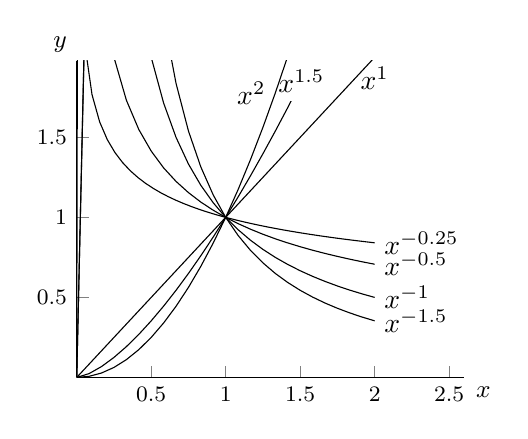
\begin{tikzpicture}
\begin{axis}[small,axis lines*=middle,ymin=0,ymax=1.98,xmin=0,xmax=2.6,xlabel={$x$},ylabel={$y$},xlabel style={at={(axis description cs:1.05,0)}},ylabel style ={rotate=-90},ylabel style={at={(axis description cs:0,1.05)}}]
\addplot[domain=0:2]{x^1.5}node[pos=0.69,fill=white]{$x^{1.5}$};
\addplot[domain=0:2]{x^2}node[pos=0.5,left]{$x^2$};
\addplot[domain=0:2]{x^1}node[below]{$x^1$};
\addplot[domain=0:2]{x^(-0.5)}node[right]{$x^{-0.5}$};
\addplot[domain=0:2,samples=40]{x^(-0.25)}node[right]{$x^{-0.25}$};
\addplot[domain=0:2]{x^(-1)}node[right]{$x^{-1}$};
\addplot[domain=0:2]{x^(-1.5)}node[right]{$x^{-1.5}$};
\end{axis}
\end{tikzpicture}
\caption*{(الف) پہلی صورت: منفرد حقیقی جذر۔}
\end{subfigure}%
\begin{subfigure}{0.5\textwidth}
\centering
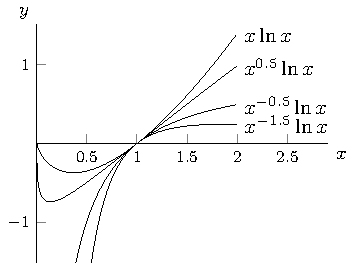
\includegraphics{figEulerCauchyABCD}
\caption*{(ب) دوسری صورت: دوہرا جذر۔}
\end{subfigure}
\begin{subfigure}{0.5\textwidth}
\centering
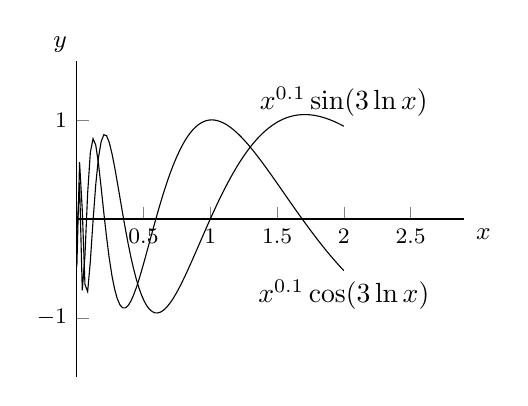
\begin{tikzpicture}
\begin{axis}[small,axis lines*=middle,ymin=-1.6,ymax=1.6,xmin=0,xmax=2.9,xlabel={$x$},ylabel={$y$},xlabel style={at={(axis description cs:1.05,0.5)}},ylabel style ={rotate=-90},ylabel style={at={(axis description cs:0,1.05)}}]
\addplot[domain=0.001:2,samples=100]{x^(0.1)*cos(180/pi*3*ln(x))}node[below]{$x^{0.1}\cos(3\ln x)$};
\addplot[domain=0.001:2,samples=100]{x^(0.1)*sin(180/pi*3*ln(x))}node[above]{$x^{0.1}\sin(3\ln x)$};
\end{axis}
\end{tikzpicture}
\caption*{(پ) جوڑی دار مخلوط جذر۔}
\end{subfigure}
\caption{یولر کوشی سادہ تفرقی مساوات کے حل۔}
\label{شکل_سادہ_دو_درجی_یولر_کوشی}
\end{figure}

شکل \حوالہ{شکل_سادہ_دو_درجی_یولر_کوشی} میں یولر کوشی سادہ تفرقی مساوات کی تینوں صورتوں کے حل دکھائے گئے ہیں۔

%============================
\ابتدا{مثال}\شناخت{مثال_سادہ_دو_ہم_محوری_نلکی_میدان}\quad دو ہم محوری نلکیوں کے بیچ میں ساکن برقی میدان؛ سرحدی قیمت مسئلہ\\
دو ہم محوری نلکیوں  کے بیچ میں برقی دباو تفرقی مساوات \عددی{\rho \tfrac{\dif^{\,2} v}{\dif \rho^2}+\tfrac{\dif v}{\dif \rho}=0} دیتی ہے۔نلکی کے رداس \عددی{\rho_1=\SI{2}{\centi\meter}} اور \عددی{\rho_2=\SI{5}{\centi\meter}} ہیں جبکہ ان پر \اصطلاح{برقی دباو}\فرہنگ{برقی دباو}\حاشیہب{electric voltage}\فرہنگ{voltage} \عددی{v_1=\SI{50}{\volt}} اور \عددی{v_2=\SI{0}{\volt}} ہے۔درمیانی خطے کی برقی دباو حاصل کریں۔

حل:یولر کوشی مساوات میں \عددی{a=1} اور \عددی{b=0} موجودہ تفرقی مساوات دیتا ہے۔دیے مساوات میں \عددی{v=\rho^m} پر کرتے ہوئے ذیلی مساوات \عددی{m^2=0} حاصل ہوتی ہے جس کا دوہرا جذر \عددی{m=0} ہے۔یوں عمومی  حل \عددی{v=c_1+c_2\ln x} ہو گا۔دیے گئے سرحدی شرائط حل میں پر کرتے 
\begin{align*}
50=c_1+c_2\ln 0.02, \quad 0=c_1+c_2\ln 0.05
\end{align*}
ہوئے \عددی{c_1=-163.471} اور \عددی{c_2=-54.568} حاصل ہوتے ہیں لہٰذا مخصوص حل \عددی{y=-163.471-54.568\ln \rho} ہو گا جسے شکل \حوالہ{شکل_مثال_سادہ_دو_ہم_محوری_نلکی_میدان} میں دکھایا گیا ہے۔
\begin{figure}
\centering
\begin{tikzpicture}
\begin{axis}[small,axis lines*=middle,ymin=0,ymax=58,xmin=0.02,xmax=0.056,xlabel={$\rho$},ylabel={$v$},xlabel style={at={(axis description cs:1.05,0)}},ylabel style ={rotate=-90},ylabel style={at={(axis description cs:0,1.05)}},scaled x ticks=false,xtick={0.02,0.03,0.04,0.05},xticklabels={$2$,$3$,$4$,$5$},ytick={0,50},yticklabels={$0$,$50$}]
\addplot[domain=0.01:0.05]{-163.471-54.568*ln(x)};
\end{axis}
\end{tikzpicture}
\caption{مثال \حوالہ{مثال_سادہ_دو_ہم_محوری_نلکی_میدان} کا حل۔}
\label{شکل_مثال_سادہ_دو_ہم_محوری_نلکی_میدان}
\end{figure}
\انتہا{مثال}
%==========================
\ابتدا{مثال}
یولر کوشی مساوات \حوالہ{مساوات_سادہ_دو_درجی_یولر_کوشی_الف} میں \عددی{x=e^{t}} پر کرتے ہوئے اس کو مستقل عددی سر والے سادہ تفرقی مساوات میں تبدیل کریں۔

حل:ہم \عددی{y(x)} کو \عددی{y[x(t)]} یعنی \عددی{y(t)} تصور کرتے ہیں۔یوں زنجیری تفرق سے
\begin{align*}
\frac{\dif y}{\dif x}=\frac{\dif y}{\dif t}\frac{\dif t}{\dif x}, \quad \frac{\dif^{\,2} y}{\dif x^2}=\frac{\dif^{\,2}y}{\dif t^2}\left(\frac{\dif t}{\dif x}\right)^2+\frac{\dif y}{\dif t}\frac{\dif^{\,2} t}{\dif x^2}
\end{align*}
لکھا جا سکتا ہے۔ان میں \عددی{\tfrac{\dif t}{\dif x}=\tfrac{1}{x}} اور \عددی{\tfrac{\dif^{\,2} t}{\dif x^2}=-\tfrac{1}{x^2}} پر کرتے ہیں۔
\begin{align*}
\frac{\dif y}{\dif x}=\frac{1}{x}\frac{\dif y}{\dif t}, \quad \frac{\dif^{\,2} y}{\dif x^2}=\frac{1}{x^2}\frac{\dif^{\,2}y}{\dif t^2}-\frac{1}{x^2}\frac{\dif y}{\dif t}
\end{align*}
انہیں مساوات \حوالہ{مساوات_سادہ_دو_درجی_یولر_کوشی_الف} میں پر کرتے 
\begin{align*}
x^2\left(\frac{1}{x^2}\frac{\dif^{\,2}y}{\dif t^2}-\frac{1}{x^2}\frac{\dif y}{\dif t}\right)+ax\left(\frac{1}{x}\frac{\dif y}{\dif t}\right)+by=0
\end{align*}
ہوئے مستقل عددی سر والا سادہ تفرقی مساوات حاصل ہوتا ہے  جہاں \عددی{\dot{y}=\tfrac{\dif y}{\dif t}} اور \عددی{\ddot{y}=\tfrac{\dif^{\,2}y}{\dif t^2}} ہیں۔
\begin{align}
\ddot{y}+(a-1)\dot{y}+by=0
\end{align}
\انتہا{مثال}
%==================================

\حصہء{سوالات}
سوال \حوالہ{سوال_سادہ_دو_یولر_کوشی_الف} تا سوال \حوالہ{سوال_سادہ_دو_یولر_کوشی_ب} حل کریں۔
%=======================

\ابتدا{سوال}\شناخت{سوال_سادہ_دو_یولر_کوشی_الف}
\begin{align*}
x^2y''-2xy'+2y=0
\end{align*}
جواب:\عددی{y=c_1x+c_2x^2}
\انتہا{سوال}
%====================
\ابتدا{سوال}
\begin{align*}
x^2y''-6y=0
\end{align*}
جواب:\عددی{y=c_1x^3+c_2x^{-2}}
\انتہا{سوال}
%==========================
\ابتدا{سوال}
\begin{align*}
x^2y''+6xy'+4y=0
\end{align*}
جواب:\عددی{y=\tfrac{c_1}{x}+\tfrac{c_2}{x^4}}
\انتہا{سوال}
%==================
\ابتدا{سوال}
\begin{align*}
x^2y''-5xy'+9y=0
\end{align*}
جواب:\عددی{y=(c_1+c_2\ln x)x^3}
\انتہا{سوال}
%==========================
\ابتدا{سوال}
\begin{align*}
x^2y''+11xy'+25y=0
\end{align*}
جواب:\عددی{y=(c_1+c_2\ln x)x^{-5}}
\انتہا{سوال}
%========================
\ابتدا{سوال}
\begin{align*}
10x^2y''+11xy'-3y=0
\end{align*}
جواب:\عددی{y=c_1\sqrt{x}+c_2x^{-\tfrac{3}{5}}}
\انتہا{سوال}
%=====================
\ابتدا{سوال}
\begin{align*}
x^2y''+0.44xy'+0.0748y=0
\end{align*}
جواب:\عددی{y=c_1x^{0.22}+c_2x^{0.34}}
\انتہا{سوال}
%======================
\ابتدا{سوال}
\begin{align*}
x^2y''+0.4xy'+0.73y=0
\end{align*}
جواب:\عددی{y=x^{0.3}[c_1\cos(0.8\ln x)+c_2\sin(0.8\ln x)]}
\انتہا{سوال}
%===================
\ابتدا{سوال}\شناخت{سوال_سادہ_دو_یولر_کوشی_ب}
\begin{align*}
x^2y''+2xy'+4.25y=0
\end{align*}
جواب:\عددی{y=x^{-0.5}[c_1\cos(2\ln x)+c_2\sin(2\ln x)]}
\انتہا{سوال}
%======================
سوال \حوالہ{سوال_سادہ_دو_یولر_کوشی_پ} تا سوال \حوالہ{سوال_سادہ_دو_یولر_کوشی_ت} ابتدائی قیمت مسئلے ہیں۔انہیں حل کریں۔

\ابتدا{سوال}\شناخت{سوال_سادہ_دو_یولر_کوشی_پ}
\begin{align*}
x^2y''-0.4xy'+0.45y=0,\quad y(1)=2,\quad y'(1)=-1
\end{align*}
جواب:\عددی{y=7\sqrt{x}-5x^{0.9}}
\انتہا{سوال}
%================================
\ابتدا{سوال}
\begin{align*}
x^2y''+1.08xy'-0.01713y=0,\quad y(1)=-1,\quad y'(1)=1
\end{align*}
جواب:\عددی{y=\tfrac{23}{18}x^{0.23}-\tfrac{41}{18}x^{-0.31}}
\انتہا{سوال}
%================================
\ابتدا{سوال}
\begin{align*}
35x^2y''+57xy'+3y=0,\quad y(1)=3,\quad y'(1)=-5
\end{align*}
جواب:\عددی{y=\tfrac{77}{4}x^{-\tfrac{3}{7}}-\tfrac{65}{4}x^{-\tfrac{1}{5}}}
\انتہا{سوال}
%================================
\ابتدا{سوال}
\begin{align*}
6x^2y''+19xy'+6y=0,\quad y(1)=-3,\quad y'(1)=1
\end{align*}
جواب:\عددی{y=\tfrac{6}{5}x^{-\tfrac{3}{2}}-\tfrac{21}{5}x^{-\tfrac{2}{3}}}
\انتہا{سوال}
%================================
\ابتدا{سوال}
\begin{align*}
25x^2y''-15xy'+16y=0,\quad y(2)=0,\quad y'(2)=1
\end{align*}
جواب:\عددی{y=2^{\tfrac{1}{5}}x^{\tfrac{4}{5}}(\ln x-\ln 2)}
\انتہا{سوال}
%================================
\ابتدا{سوال}\شناخت{سوال_سادہ_دو_یولر_کوشی_ت}
\begin{align*}
49x^2y''+77xy'+4y=0,\quad y(2)=3,\quad y'(2)=0
\end{align*}
جواب:\عددی{y=x^{-\tfrac{2}{7}}(2.93+1.04\ln x)}
\انتہا{سوال}
%================================

\حصہ{حل کی وجودیت اور یکتائی؛ ورونسکی}\شناخت{حصہ_سادہ_دو_وجودیت_یکتائی_ورونسکی}
اس حصے میں متجانس خطی سادہ تفرقی مساوات،
\begin{align}\label{مساوات_سادہ_دو_وجودیت_مخصوص_الف}
y''+p(x)y'+q(x)y=0
\end{align}
جس کے عددی سر \عددی{p(x)} اور \عددی{q(x)} کوئی بھی \اصطلاح{استمراری تفاعل} ہو سکتے  ہیں، کے عمومی حل کی \اصطلاح{وجودیت}\فرہنگ{وجودیت}\حاشیہب{existence}\فرہنگ{existence} پر غور کیا جائے گا۔ساتھ ہی ساتھ مساوات \حوالہ{مساوات_سادہ_دو_وجودیت_مخصوص_الف} اور  ابتدائی معلومات
\begin{align}\label{مساوات_سادہ_دو_وجودیت_مخصوص_ب}
y(x_0)=K_0, \quad y'(x_0)=K_1
\end{align}
کے  ابتدائی قیمت مسئلہ کی مخصوص حل کی \اصطلاح{یکتائی}\فرہنگ{یکتائی}\حاشیہب{uniqueness}\فرہنگ{uniqueness} پر بحث کی جائے گی۔ 

مسئلہ \حوالہ{مسئلہ_سادہ_دو_درجی_یکتا_مخصوص_حل} کہتا ہے کہ اس ابتدائی قیمت مسئلے کا مخصوص حل پایا جاتا ہے جو یکتا ہو گا اور مساوات \حوالہ{مساوات_سادہ_دو_وجودیت_مخصوص_الف} کے عمومی حل
\begin{align}
y=c_1y_1+c_2y_2\quad \quad \text{\RL{اختیاری $c_1$, $c_2$}}
\end{align}
میں تمام حل شامل ہیں۔یوں استمراری عددی سر والے متجانس سادہ تفرقی مساوات کا کوئی \اصطلاح{نادر حل}\فرہنگ{نادر حل}\فرہنگ{حل!نادر} نہیں پایا جاتا۔نادر حل اس حل کو کہتے ہیں جسے عمومی حل سے حاصل نہیں کیا جا سکتا ہے۔

ہمیں مستقل عددی سر والے سادہ تفرقی مساوات یا یولر کوشی سادہ تفرقی مساوات کے حل کی وجودیت اور یکتائی جاننے کی ضرورت پیش نہیں آئی چونکہ ان کے حل کے دوران ہی ایسی تمام معلومات سامنے آ جاتی ہیں۔
%================

%\theoremstyle{plain}
%\begin{theorem}[]\label{مسئلہ_سادہ_دو_درجی_یکتا_مخصوص_حل}
\ابتدا{مسئلہ}\شناخت{مسئلہ_سادہ_دو_درجی_یکتا_مخصوص_حل}\quad مسئلہ وجودیت اور یکتائی برائے ابتدائی قیمت تفرقی مساوات\فرہنگ{مسئلہ!وجودیت اور یکتائی}\\
اگر \عددی{p(x)} اور \عددی{q(x)} کسی کھلے  وقفے \عددی{I} پر استمراری ہوں اور \عددی{x_0} اس وقفے پر پایا جاتا ہو، تب مساوات \حوالہ{مساوات_سادہ_دو_وجودیت_مخصوص_الف} اور مساوات \حوالہ{مساوات_سادہ_دو_وجودیت_مخصوص_ب} پر مبنی ابتدائی قیمت مسئلے کا \عددی{I} پر  یکتا مخصوص حل \عددی{y(x)}  موجود ہے۔  
%\end{theorem}
\انتہا{مسئلہ}
%============================

وجودیت حل کی ثبوت کے لئے وہی بنیادی شرائط درکار ہیں جو صفحہ \حوالہصفحہ{مسئلہ_سادہ_اول_وجودیت} پر مسئلہ \حوالہ{مسئلہ_سادہ_اول_وجودیت} کے لئے درکار تھے۔اس کتاب میں ان پر غور نہیں کیا جائے گا۔ اگرچہ یکتائی کا ثبوت عموماً آسان ہوتا ہے لیکن موجودہ مسئلہ \حوالہ{مسئلہ_سادہ_دو_درجی_یکتا_مخصوص_حل} کے یکتائی حل کا ثبوت اتنا آسان نہیں ہے لہٰذا اس کو کتاب کے آخر میں بطور ضمیمہ \حوالہ{ضمیمہ_اضافی_ثبوت} شامل کیا گیا ہے۔ 
%==================

\جزوحصہء{خطی طور غیر تابع حل}
آپ کو حصہ \حوالہ{حصہ_سادہ_اسپرنگ_کمیت} سے یاد ہو گا کہ کھلے وقفہ \عددی{I} پر عمومی حل \اصطلاح{اساس} \عددی{y_1}، \عددی{y_2} پر مشتمل ہوتا ہے جہاں \عددی{y_1} اور \عددی{y_2} کھلے وقفے \عددی{I} پر خطی طور غیر تابع حل ہیں۔ وقفہ \عددی{I} پر معین \عددی{y_1} اور \عددی{y_2}،  وقفہ \عددی{I}  پر، اس صورت \اصطلاح{خطی طور غیر تابع}\فرہنگ{خطی طور! غیر تابع}\حاشیہب{linearly independent}\فرہنگ{linearly independent} کہلاتے ہیں جب پورے وقفے پر
\begin{align}\label{مساوات_سادہ_دو_خطی_طور_غیر_تابع_الف}
k_1 y_1+k_2 y_2=0
\end{align}
سے مراد 
\begin{align}
k_1=0, \quad k_2=0
\end{align}
ہو۔\عددی{k_1} اور \عددی{k_2} میں سے کم از کم ایک کی قیمت صفر کے برابر نہ ہونے کی صورت میں مساوات \حوالہ{مساوات_سادہ_دو_خطی_طور_غیر_تابع_الف} پر پورا اترتے ہوئے حل \عددی{y_1} اور \عددی{y_2} \اصطلاح{خطی طور تابع}\فرہنگ{خطی طور!تابع}\حاشیہب{linearly dependent}\فرہنگ{linearly dependent} کہلاتے ہیں۔اگر \عددی{k_1 \ne 0} ہو تب ہم مساوات \حوالہ{مساوات_سادہ_دو_خطی_طور_غیر_تابع_الف} کو \عددی{k_1} سے تقسیم کرتے ہوئے \عددی{y_1=-\tfrac{k_2}{k_1}y_2} لکھ سکتے ہیں جو تناسبی رشتہ ہے۔اسی طرح \عددی{k_2 \ne 0} کی صورت میں \عددی{y_2=-\tfrac{k_1}{k_2}y_1} لکھا جا سکتا ہے جو تناسبی رشتے کو ظاہر کرتی ہے۔
\begin{align}\label{مساوات_سادہ_دور_خطی_غیر_تابع_شرط}
\text{(الف)}\quad y_1=ky_2,\quad \text{(ب)}\quad y_2=l y_1 \quad \quad \text{\RL{پورے $I$ پر}}
\end{align}
اس کے برعکس خطی طور غیر تابعیت کی صورت میں ہم مساوات \حوالہ{مساوات_سادہ_دو_خطی_طور_غیر_تابع_الف} کو \عددی{k_1} (یا \عددی{k_2}) سے تقسیم نہیں کر سکتے لہٰذا  تناسبی رشتہ حاصل نہیں کیا جا سکتا۔(درج بالا مساوات میں \عددی{k=-\tfrac{k_2}{k_1}} اور \عددی{l=-\tfrac{k_1}{k_2}} لکھے گئے ہیں۔\عددی{k} یا (اور) \عددی{l} صفر بھی ہو سکتے ہیں۔) خطی طور غیر تابع اور خطی طور تابع حل کو درج ذیل طرز پر بیان کیا جا سکتا ہے۔ 
%==========================

%\begin{theorem}[خطی طور تابع اور غیر تابع حل]
\ابتدا{مسئلہ}\شناخت{مسئلہ_سادہ_دو_حل_تابع_غیر_تابع}\quad خطی طور تابع اور غیر تابع حل\فرہنگ{مسئلہ!تابع اور غیر تابع حل}\\
کھلے وقفہ \عددی{I} پر استمراری  \عددی{p(x)} اور \عددی{q(x)} عددی سر والے سادہ تفرقی  مساوات \حوالہ{مساوات_سادہ_دو_خطی_طور_غیر_تابع_الف} کے \عددی{I}  پر دو حل \عددی{y_1} اور \عددی{y_2} اس صورت \اصطلاح{خطی طور تابع}\فرہنگ{خطی طور تابع}\فرہنگ{linearly dependent} ہوں گے جب ان کے \اصطلاح{ورونسکی}\فرہنگ{ورونسکی}\حاشیہب{Wronskian}\فرہنگ{Wronskian}
\begin{align}\label{مساوات_سادہ_دو_ورونسکی_تعریف}
W(y_1,y_2)=y_1y_2'-y_2y_1'
\end{align}
کی قیمت  کسی \عددی{x_0} پر صفر کے برابر ہو، جہاں \عددی{x_0} کھلے وقفے \عددی{I} پر پایا جاتا ہے۔مزید اگر  نقطہ \عددی{x=x_0} پر \عددی{W=0} ہو تب پورے \عددی{I} پر \عددی{W} \اصطلاح{مکمل صفر}\فرہنگ{مکمل صفر}\فرہنگ{صفر!مکمل}\حاشیہب{identically zero}\فرہنگ{identically zero} ہو گا۔یوں اگر \عددی{I} پر کوئی ایسا \عددی{x} پایا جاتا ہو جس پر \عددی{W} صفر کے برابر نہ ہو تب \عددی{y_1} اور \عددی{y_2} \اصطلاح{خطی طور غیر تابع}\فرہنگ{خطی طور غیر تابع}\فرہنگ{linearly independent} ہوں گے۔
%\end{theorem}
\انتہا{مسئلہ}
%==================
\ابتدا{ثبوت}
\begin{enumerate}
\item[(الف)]
\عددی{y_1} اور \عددی{y_2} کو \عددی{I} پر خطی طور غیر تابع تصور کریں۔یوں مساوات \حوالہ{مساوات_سادہ_دور_خطی_غیر_تابع_شرط}-الف یا ب میں سے ایک درست ہو گا۔اگر  مساوات \حوالہ{مساوات_سادہ_دور_خطی_غیر_تابع_شرط}-الف  درست ہو تب
\begin{align*}
W(y_1,y_2)=y_1y_2'-y_2y_1'=ky_2y_2'-y_2ky_2'=0
\end{align*}
ہو گا۔اسی طرح مساوات \حوالہ{مساوات_سادہ_دور_خطی_غیر_تابع_شرط}-ب کی صورت میں بھی \عددی{W=0} ملتا ہے۔
\item[(ب)]
 اس کے الٹ چلتے ہوئے ہم ثابت کرتے ہیں کہ کسی \عددی{x_0} پر \عددی{W(y_1,y_2)=0} سے مراد \عددی{y_1} اور \عددی{y_2} کا \عددی{I} پر خطی طور تابع ہونا ہے۔درج ذیل مساوات پر غور کریں جہاں \عددی{k_1} اور \عددی{k_2} کو نا معلوم متغیرات تصور کریں۔
\begin{gather}
\begin{aligned}\label{مساوات_سادہ_دو_درجی_ثبوت_الف}
k_1y_1(x_0)+k_2y_2(x_0)&=0\\
k_1y_1'(x_0)+k_2y_2'(x_0)&=0
\end{aligned}
\end{gather}
\عددی{k_2} حذف کرنے کی نیت سے  پہلی مساوات کو \عددی{y_2'(x_0)} اور دوسری کو \عددی{-y_2(x_0)} سے ضرب دیتے ہوئے دونوں کا مجموعہ لیتے ہیں۔
\begin{align}\label{مساوات_سادہ_دو_درجی_ثبوت_ب}
k_1y_1(x_0)y_2'(x_0)-k_1y_1'(x_0)y_2(x_0)=k_1W(y_1(x_0),y_2(x_0))=0
\end{align}
اسی طرح \عددی{k_1} حذف کرنے کے لئے پہلی مساوات کو \عددی{-y_1'(x_0)} اور دوسری کو \عددی{y_1(x_0)} سے ضرب دیتے ہوئے دونوں مساوات کا مجموعہ
\begin{align}\label{مساوات_سادہ_دو_درجی_ثبوت_پ}
k_2y_1(x_0)y_2'(x_0)-k_2y_2(x_0)y_1'(x_0)=k_2W(y_1(x_0),y_2(x_0))=0
\end{align}
لیتے ہیں۔اب اگر \عددی{x_0} پر \عددی{W} صفر نہ ہوتا تب ہم مساوات \حوالہ{مساوات_سادہ_دو_درجی_ثبوت_ب} اور مساوات \حوالہ{مساوات_سادہ_دو_درجی_ثبوت_پ} کو \عددی{W} سے تقسیم کرتے ہوئے \عددی{k_1=k_2=0} حاصل کرتے البتہ \عددی{x_0} پر \عددی{W(y_1(x_0),y_2(x_0))=0} ہے لہٰذا ہم ان مساوات کو \عددی{W} سے  تقسیم نہیں کر سکتے ہیں۔ یوں  ہمزاد مساوات \حوالہ{مساوات_سادہ_دو_درجی_ثبوت_الف} کا حل \عددی{k_1} اور \عددی{k_2} پایا جاتا ہے جہاں \عددی{k_1} اور \عددی{k_2} دونوں غیر صفر ہو سکتے ہیں۔ اب ان اعداد \عددی{k_1} اور \عددی{k_2} کو استعمال کرتے ہوئے تفاعل
\begin{align}
y(x)=k_1y_1(x)+k_2y_2(x)
\end{align}
لیتے ہیں۔چونکہ مساوات \حوالہ{مساوات_سادہ_دو_وجودیت_مخصوص_الف} متجانس خطی ہے لہٰذا  مسئلہ \حوالہ{مسئلہ_دو_درجی_خطی_میل}  (مسئلہ خطی میل) کے تحت  یہ تفاعل بھی مساوات \حوالہ{مساوات_سادہ_دو_وجودیت_مخصوص_الف} کا حل ہو گا۔مساوات \حوالہ{مساوات_سادہ_دو_درجی_ثبوت_الف} سے ظاہر ہے کہ یہ تفاعل ابتدائی معلومات \عددی{y(x_0)=0} اور \عددی{y'(x_0)=0} پر پورا اترتا ہے۔اب تصور کریں کہ مساوات \حوالہ{مساوات_سادہ_دو_وجودیت_مخصوص_الف} کا دوسرا حل جو انہیں  ابتدائی معلومات پر پورا اترتا ہو \عددی{y^*(x)=0} ہے۔اب چونکہ مساوات \حوالہ{مساوات_سادہ_دو_وجودیت_مخصوص_الف} میں \عددی{p(x)} اور \عددی{q(x)} استمراری ہیں لہٰذا مسئلہ \حوالہ{مسئلہ_سادہ_دو_درجی_یکتا_مخصوص_حل} کے تحت اس کا مخصوص حل یکتا ہو گا۔یوں \عددی{y(x)} اور \عددی{y^*(x)} مختلف نہیں ہو سکتے ہیں لہٰذا \عددی{y^*(x)=y(x)=0} یعنی
\begin{align}\label{مساوات_سادہ_دو_درجی_ثبوت_ت}
k_1y_1+k_2y_2\equiv 0\quad \quad \text{\RL{پورے $I$ پر}}
\end{align}
ہو گا۔چونکہ \عددی{k_1} اور \عددی{k_2} میں کم از کم ایک صفر کے برابر نہیں ہے لہٰذا  مساوات \حوالہ{مساوات_سادہ_دو_درجی_ثبوت_ت} کہتا ہے کہ \عددی{I} پر \عددی{y_1} اور \عددی{y_2} خطی طور تابع ہیں۔
\item[(پ)]
ہم مسئلے کا آخری نقطہ ثابت کرتے ہیں۔اگر کھلے وقفے \عددی{I} پر نقطہ \عددی{x_0} پر \عددی{W(x_0)=0} ہو تب ثبوت (ب) کے تحت \عددی{I} پر \عددی{y_1} اور \عددی{y_2} خطی طور تابع ہیں لہٰذا ثبوت (الف) کے تحت \عددی{W \equiv 0} ہو گا۔یوں خطی طور تابعیت کی صورت میں ایسا نہیں ہو سکتا ہے کہ \عددی{W(x_1) \ne 0} ہو جہاں \عددی{x_1} کھلے وقفہ \عددی{I} پر پایا جاتا ہے۔اگر ایسا ممکن ہو تب اس سے مراد خطی طور غیر تابعیت ہو گی جیسا کہ دعویٰ کیا گیا ہے۔ 
\end{enumerate}
\انتہا{ثبوت}
%=================

حساب کی نقطہ نظر سے  مساوات \حوالہ{مساوات_سادہ_دو_ورونسکی_تعریف} سے درج ذیل زیادہ آسان مساوات ہے۔
\begin{align}\label{مساوات_سادہ_دو_آسان_ورونسکی}
W(y_1,y_2)=
\begin{cases}
\left(\frac{y_2}{y_1}\right)^{\!'}y_1^2  &(y_1 \ne 0)\\[0.5em]
-\left(\frac{y_1}{y_2}\right)^{\!'}y_2^2 & (y_2 \ne 0)
\end{cases}
\end{align}
آپ دیکھ سکتے ہیں کہ  ورونسکی کو قالب کی مقطع کے طرز پر لکھا جا سکتا ہے جس کو \اصطلاح{ورونسکی مقطع}\فرہنگ{ورونسکی!مقطع}\فرہنگ{مقطع!ورونسکی}\حاشیہب{Wronskian determinant}\فرہنگ{Wronskian determinant} یا حل \عددی{y_1} اور \عددی{y_2} کی \اصطلاح{ورونسکی} کہتے ہیں۔ 
\begin{align}
W(y_1,y_2)=
\begin{vmatrix}
y_1 &y_2\\[0.25em]
y_1' & y_2'
\end{vmatrix}
=y_1y_2'-y_2y_1'
\end{align}
%==============================

\ابتدا{مثال}\quad مسئلہ \حوالہ{مسئلہ_سادہ_دو_حل_تابع_غیر_تابع} کا اطلاق\\
تفرقی مساوات \عددی{y''+\omega^2y=0} کے حل \عددی{y_1=\cos \omega x} اور \عددی{y_2=\sin \omega x}  ہیں۔ان کی ورونسکی
\begin{align*}
W(\cos \omega x,\sin \omega x)=
\begin{vmatrix}
\cos \omega x &\sin \omega x\\[0.25em]
-\omega \sin \omega x & -\omega \cos \omega x
\end{vmatrix}
=\omega \cos^2 \omega x+\omega \sin^2 \omega x=\omega
\end{align*}
ہے۔مسئلہ \حوالہ{مسئلہ_سادہ_دو_حل_تابع_غیر_تابع} کے تحت یہ حل صرف اس صورت میں خطی طور غیر تابع ہوں گے جب \عددی{\omega \ne 0} ہو۔یہی دونوں حل کے حاصل تقسیم \عددی{\tfrac{y_2}{y_1}=\tan \omega x} سے بھی اخذ کیا جا سکتا ہے جہاں \عددی{\omega=0} سے \عددیء{y_2=0} ملتا ہے جو خطی طور تابع صورت ظاہر کرتی ہے۔
\انتہا{مثال}
%=============================
\ابتدا{مثال}\quad دوہرا جذر کی صورت میں مسئلہ \حوالہ{مسئلہ_سادہ_دو_حل_تابع_غیر_تابع} کا اطلاق\\
تفرقی مساوات \عددی{y''-6y'+9y=0} کا (ثابت کریں کہ) عمومی حل  \عددی{y=(c_1+c_2 x)e^{3x}}   ہے جس کا ورونسکی صفر کے برابر نہیں ہے لہٰذا \عددی{e^{3x}} اور \عددی{xe^{3x}} تمام \عددی{x} پر خطی طور غیر تابع ہیں۔
\begin{align*}
W(e^{3x},xe^{3x})=
\begin{vmatrix}
e^{3x}& xe^{3x}\\[0.25em]
3e^{3x}&e^{3x}+3xe^{3x}
\end{vmatrix}
=e^{6x}+3xe^{6x}-3xe^{6x}=e^{6x} \ne 0
\end{align*}
\انتہا{مثال}
%==================

\جزوحصہء{مساوات \حوالہ{مساوات_سادہ_دو_وجودیت_مخصوص_الف} کے عمومی حل میں تمام حل کی شمولیت}
اس حصے کو مساوات \حوالہ{مساوات_سادہ_دو_وجودیت_مخصوص_الف} کے عمومی حل کی وجودیت سے شروع کرتے ہیں۔
%=========================

\ابتدا{مسئلہ}\شناخت{مسئلہ_سادہ_دو_وجودیت_الف}\quad \اصطلاح{وجودیت عمومی حل}\فرہنگ{وجودیت!عمومی حل}\فرہنگ{حل!وجودیت عمومی حل}\فرہنگ{existence!solution}\فرہنگ{مسئلہ!وجودیت عمومی حل}\\
کھلے وقفہ \عددی{I} پر استمراری \عددی{p(x)} اور \عددی{q(x)} کی صورت میں مساوات \حوالہ{مساوات_سادہ_دو_وجودیت_مخصوص_الف} کا عمومی حل \عددی{I} پر موجود ہے۔
\انتہا{مسئلہ}
%=====================

\ابتدا{ثبوت}
مسئلہ \حوالہ{مسئلہ_سادہ_دو_درجی_یکتا_مخصوص_حل} کے تحت  \عددی{I} پر مساوات \حوالہ{مساوات_سادہ_دو_وجودیت_مخصوص_الف} کا، ابتدائی معلومات 
\begin{align*}
y_1(x_0)=1, \quad y_1'(x_0)=0
\end{align*}
پر پورا اترتا ہوا  حل  \عددی{y_1(x)} موجود ہے۔اسی طرح ابتدائی معلومات
\begin{align*}
y_2(x_0)=0, \quad y_2'(x_0)=1
\end{align*}
 پر پورا اترتا ہوا  حل \عددی{y_2(x)} بھی موجود ہے۔نقطہ \عددی{x_0} پر ان کا ورونسکی
\begin{align*}
W(y_1(x_0),y_2(x_0))=y_1(x_0)y'_2(x_0)-y_2(x_0)y'_1(x_0)=1
\end{align*}
ہے۔مسئلہ \حوالہ{مسئلہ_سادہ_دو_حل_تابع_غیر_تابع} کے تحت \عددی{I} پر \عددی{y_1} اور \عددی{y_2} خطی طور غیر تابع ہیں لہٰذا یہ مساوات \حوالہ{مساوات_سادہ_دو_وجودیت_مخصوص_الف} کے حل کی اساس ہیں۔اس طرح ثابت ہوا کہ  \عددی{I} پر  مساوات \حوالہ{مساوات_سادہ_دو_وجودیت_مخصوص_الف} کا عمومی حل \عددی{y=c_1y_1+c_2y_2} ہے جہاں \عددی{c_1} اور \عددی{c_2} اختیاری مستقل ہیں۔
\انتہا{ثبوت}
%=======================

آئیں اب ثابت کریں کہ عمومی حل اتنا عمومی ہے جتنا کوئی حل عمومی ہو سکتا ہے۔
%=====================

\ابتدا{مسئلہ}\quad عمومی حل میں تمام حل شامل ہیں\\
کھلا وقفہ \عددی{I} پر استمراری \عددی{p(x)} اور \عددی{q(x)} کی صورت میں \عددی{I} پر مساوات \حوالہ{مساوات_سادہ_دو_وجودیت_مخصوص_الف} کے ہر حل
 \عددی{y=Y(x)} کو
\begin{align}
Y(x)=C_1y_1+C_2y_2
\end{align}
لکھا جا سکتا ہے، جہاں \عددی{y_1} اور \عددی{y_2} کھلے وقفہ \عددی{I} پر مساوات \حوالہ{مساوات_سادہ_دو_وجودیت_مخصوص_الف} کی کوئی بھی اساس اور \عددی{C_1}، \عددی{C_2} مناسب مستقل ہیں۔

یوں مساوات \حوالہ{مساوات_سادہ_دو_وجودیت_مخصوص_الف} کا کوئی \اصطلاح{نادر حل}\فرہنگ{نادر حل} موجود نہیں ہے۔(نادر حل سے مراد ایسا حل ہے جس کو عمومی حل سے حاصل نہیں کیا جا سکتا ہے۔)
\انتہا{مسئلہ}
%======================

\ابتدا{ثبوت}
تصور کریں کہ \عددی{I} پر مساوات \حوالہ{مساوات_سادہ_دو_وجودیت_مخصوص_الف} کا  \عددی{y=Y(x)} کوئی حل ہے۔اب مسئلہ \حوالہ{مسئلہ_سادہ_دو_وجودیت_الف} کے تحت \عددی{I} پر  تفرقی مساوات \حوالہ{مساوات_سادہ_دو_وجودیت_مخصوص_الف} کا عمومی حل
\begin{align}\label{مساوات_سادہ_دو_ثبوت_مسئلہ_چار_الف}
y(x)=c_1y_1(x)+c_2y_2(x)
\end{align}
موجود ہے۔ہم \عددی{c_1} اور \عددی{c_2} کی وہ قیمتیں دریافت کرنا چاہتے ہیں جن سے \عددی{I} پر  \عددی{y(x)=Y(x)} حاصل ہوتا ہو۔ہم \عددی{I} پر کوئی بھی \عددی{x_0} چنتے ہوئے پہلے ثابت کرتے ہیں کہ \عددی{c_1} اور \عددی{c_2} کی ایسی قیمتیں دریافت کی جا سکتی ہیں کہ \عددی{x_0} پر \عددی{y(x_0)=Y(x_0)} اور 
\عددی{y'(x_0)=Y'(x_0)} ہوں۔اس کو مساوات \حوالہ{مساوات_سادہ_دو_ثبوت_مسئلہ_چار_الف} کے استعمال سے 
\begin{align}
c_1y_1(x_0)+c_2y_2(x_0)&=Y(x_0)\label{مساوات_سادہ_دو_ثبوت_مسئلہ_چار_ب}\\
c_1y'_1(x_0)+c_2y'_2(x_0)&=Y'(x_0)\label{مساوات_سادہ_دو_ثبوت_مسئلہ_چار_پ}
\end{align}
لکھ سکتے ہیں۔ان ہمزاد مساوات سے \عددی{c_1} اور \عددی{c_2} معلوم کرتے ہیں۔مساوات \حوالہ{مساوات_سادہ_دو_ثبوت_مسئلہ_چار_ب} کو \عددی{y'_2(x_0)} اور مساوات \حوالہ{مساوات_سادہ_دو_ثبوت_مسئلہ_چار_پ} کو \عددی{-y_2(x_0)} سے ضرب دیتے ہوئے مجموعہ لینے سے \عددی{c_1} حاصل کیا جا سکتا ہے۔ایسا کرنے سے مساوات \حوالہ{مساوات_سادہ_دو_ثبوت_مسئلہ_چار_ت} ملتی ہے۔اسی طرح \عددی{c_2} حاصل کرنے کی خاطر پہلی مساوات کو \عددی{-y'_1(x_0)} اور دوسری کو \عددی{y_1(x_0)} سے ضرب دیتے ہوئے مجموعہ لیتے ہوئے مساوات \حوالہ{مساوات_سادہ_دو_ثبوت_مسئلہ_چار_ٹ} حاصل ہوتی ہے۔ان مساوات میں \عددی{y_1}، \عددی{y'_1}، \عددی{y_2}،\عددی{y'_2}، \عددی{Y} اور \عددی{Y'} کی قیمتیں نقطہ \عددی{x_0} پر لی گئی ہیں۔ 
\begin{align}
c_1y_1y'_2-c_1y_2y'_1&=c_1W(y_1,y_2)=Yy_2'-y_2Y\label{مساوات_سادہ_دو_ثبوت_مسئلہ_چار_ت}\\
c_2y_1y'_2-c_2y_2y'_1&=c_2W(y_1,y_2)=y_1Y-Yy'_1\label{مساوات_سادہ_دو_ثبوت_مسئلہ_چار_ٹ}
\end{align}
اب چونکہ \عددی{y_1} اور \عددی{y_2} حل کی اساس ہیں لہٰذا ورونسکی کی قیمت صفر کے برابر نہیں ہے لہٰذا ان مساوات سے \عددی{c_1} اور \عددی{c_2} حاصل کیے جا سکتے ہیں
\begin{align*}
c_1=\frac{Yy_2'-y_2Y}{W}=C_1, \quad c_2=\frac{y_1Y-Yy'_1}{W}=C_2
\end{align*}
جہاں ان منفرد قیمتوں کو \عددی{C_1} اور \عددی{C_2} لکھا گیا ہے۔ انہیں مساوات \حوالہ{مساوات_سادہ_دو_ثبوت_مسئلہ_چار_الف} میں پر کرتے ہوئے مخصوص حل
\begin{align*}
y^*(x)=C_1y_1(x)+C_2y_2(x)
\end{align*}
حاصل ہوتا ہے۔اب چونکہ \عددی{C_1} اور \عددی{C_2} مساوات \حوالہ{مساوات_سادہ_دو_ثبوت_مسئلہ_چار_ب} اور مساوات \حوالہ{مساوات_سادہ_دو_ثبوت_مسئلہ_چار_پ} کے حل ہیں لہٰذا ہم ان مساوات سے دیکھتے ہیں کہ
\begin{align*}
y^{*}(x_0)=Y(x_0),\quad y^{*'}(x_0)=Y'(x_0)
\end{align*}
مسئلہ \حوالہ{مسئلہ_سادہ_دو_درجی_یکتا_مخصوص_حل} میں جس یکتائی کا ذکر کیا گیا ہے اس کے تحت \عددی{y^*} اور \عددی{Y} تمام \عددی{I} پر ہر جگہ برابر ہوں گے۔
\انتہا{ثبوت}
%=========================

\حصہء{سوالات}
%===================

\ابتدا{سوال}
مساوات \حوالہ{مساوات_سادہ_دو_آسان_ورونسکی} سے مساوات \حوالہ{مساوات_سادہ_دو_ورونسکی_تعریف} حاصل کریں۔
\انتہا{سوال}
%===========================
سوال \حوالہ{سوال_سادہ_ورونسکی_الف} تا سوال \حوالہ{سوال_سادہ_ورونسکی_ب} کی ورونسکی حاصل کریں۔حاصل تقسیم سے ثابت کریں کہ یہ خطی طور غیر تابع ہیں اور مسئلہ \حوالہ{مسئلہ_سادہ_دو_حل_تابع_غیر_تابع} سے  بھی اس بات کی تصدیق کریں

%======================
\ابتدا{سوال}\شناخت{سوال_سادہ_ورونسکی_الف}\quad $e^{2x}, e^{-1.2x}$\\
جوابات:\عددی{\tfrac{e^{2x}}{e^{-1.2x}}=e^{3.2x} \ne c}، \عددی{W=-3.2e^{0.8x}\ne 0}
\انتہا{سوال}
%============================ 
\ابتدا{سوال}\quad $e^{2.4x}, e^{1.1x}$\\
جوابات:\عددی{\tfrac{y_1}{y_2}=e^{1.3x} \ne c}، \عددی{W=-1.3e^{3.5x} \ne 0}
\انتہا{سوال}
%===============
\ابتدا{سوال}\quad
$x, \frac{1}{x}$\\
جوابات:\عددی{\tfrac{y_1}{y_2}=x^2 \ne c}، \عددی{W=-2x^{-2} \ne 0}
\انتہا{سوال}
%=====================
\ابتدا{سوال}\quad
$x, x^3$\\
جوابات:\عددی{\tfrac{y_1}{y_2}=x^{-2} \ne c}، \عددی{W=2x^3 \ne 0}
\انتہا{سوال}
%===================
\ابتدا{سوال}\quad
$e^{-0.2x}\sin 3x, e^{-0.2x} \cos 3x$\\
جوابات:\عددی{\tfrac{y_1}{y_2}=\tan 3x \ne c}، \عددی{W=3e^{-0.4x} \ne 0}
\انتہا{سوال}
%========================
\ابتدا{سوال}\quad
$e^{-ax}\sinh kx, e^{-ax} \cosh kx$\\
جوابات:\عددی{\tfrac{y_1}{y_2}=\tanh kx \ne c}، \عددی{W=-ke^{-2ax} \ne 0}
\انتہا{سوال}
%============================
\ابتدا{سوال}\شناخت{سوال_سادہ_ورونسکی_ب}\quad
$x^{a}\sin(k\ln x), x^{a}\cos(k\ln x)$\\
جوابات:\عددی{\tfrac{y_1}{y_2}=\tan(k \ln x) \ne c}، \عددی{W=-kx^{2a-1} \ne 0}
\انتہا{سوال}
%===========================

سوال \حوالہ{سوال_سادہ_ورونسکی_پ} تا سوال \حوالہ{سوال_سادہ_ورونسکی_ت} میں تفرقی مساوات کے حل دیے گئے ہیں۔تفرقی مساوات حاصل کریں۔ورونسکی کی مدد سے ثابت کریں کہ دیے گئے حل خطی طور غیر تابع ہیں اور ابتدائی قیمت مسئلے کا مخصوص حل حاصل کریں۔
%==============================

\ابتدا{سوال}\شناخت{سوال_سادہ_ورونسکی_پ}\quad 
$\sin 3x, \, \cos 3x,\quad y(0)=2,\quad y'(0)=-3 $\\
جوابات:\عددی{y''+9y=0}، \عددی{W=-3\ne 0}، \عددی{y=2\cos 3x-\sin 3x}
\انتہا{سوال}
%===========================
\ابتدا{سوال}\quad 
$x^3, \, x^{-4},\quad y(1)=-1,\quad y'(1)=2 $\\
جوابات:\عددی{x^2y''+2xy'-12y=0}، \عددی{W=-\tfrac{7}{x^2}\ne 0}، \عددی{y=-\tfrac{2x^3}{7}-\tfrac{5x^{-4}}{7}}
\انتہا{سوال}
%===========================
\ابتدا{سوال}\quad 
$e^{-1.2x}\sin 0.8x, \, e^{-1.2x}\cos 0.8 x,\quad y(0)=5,\quad y'(0)=7 $\\
جوابات:\عددی{y''+2.4y'+2.08y=0}، \عددی{W=-0.8e^{-2.4x} \ne 0}، \\
\عددی{y=e^{-\tfrac{6}{5}x}(\tfrac{65}{4}\sin\tfrac{4x}{5}+5\cos\tfrac{4x}{5})}
\انتہا{سوال}
%===========================
\ابتدا{سوال}\quad 
$x^3,\, x^3\ln x,\quad y(1)=2,\quad y'(1)=8 $\\
جوابات:\عددی{x^2y''-5xy'+9y=0}، \عددی{W=x^5 \ne 0}، \عددی{y=2x^3(1+\ln x)}
\انتہا{سوال}
%===========================
\ابتدا{سوال}\quad 
$1,\, e^{3x},\quad y(0)=1.5,\quad y'(0)=-2.5 $\\
جوابات:\عددی{y''-3y'=0}، \عددی{W=3e^{3x} \ne 0}، \عددی{y=\tfrac{8}{3}e^{3x}-\tfrac{2}{3}}
\انتہا{سوال}
%===========================
\ابتدا{سوال}\quad 
$e^{-kx}\sin \pi x, \, e^{-kx}\cos \pi x,\quad y(0)=1,\quad y'(0)=-k-\pi $\\
جوابات:\عددی{y''+2ky'+(k^2+\pi^2)y=0}، \عددی{W=-\pi e^{-2kx} \ne 0}، \\
\عددی{y=e^{-kx}(\sin \pi x-\cos \pi x)}
\انتہا{سوال}
%===========================
\ابتدا{سوال}\شناخت{سوال_سادہ_ورونسکی_ت}\quad 
$\sinh 1.8x, \,\cosh 1.8x,\quad y(0)=14.2,\quad y'(0)=16.38 $\\
جوابات:\عددی{y''-3.24y=0}، \عددی{W=-1.8 \ne 0}، \\
\عددی{y=9.1\sinh 1.8x+14.2\cosh 1.8x}
\انتہا{سوال}
%===========================
\ابتدا{سوال}
تفرقی مساوات \عددی{y''-y=0} کا عمومی حل قوت نمائی تفاعل اور \اصطلاح{بذلولی}\فرہنگ{بذلولی}\حاشیہب{hyperbolic}\فرہنگ{hyperbolic!function} تفاعل کی صورت میں لکھیں۔دونوں صورتوں کے مستقل کا تعلق کیا ہے؟

جوابات:\عددی{y=c_1e^{x}+c_2e^{-x}}، \عددی{y=c_a\sinh x+c_b\cosh x}، \عددی{c_a=c_1-c_2}، \عددی{c_b=c_1+c_2}
\انتہا{سوال}
%=============================
%=====================================

\حصہ{غیر متجانس سادہ تفرقی مساوات}\شناخت{حصہ_سادہ_دو_غیر_متجانس}
اس باب میں اب تک متجانس خطی سادہ تفرقی مساوات پر غور کیا گیا۔یہاں سے باب کے اختتام تک غیر متجانس خطی سادہ تفرقی مساوات پر غور کیا جائے گا۔درج ذیل غیر متجانس خطی تفرقی مساوات پر غور کرتے ہیں جہاں \عددی{r \not \equiv 0} ہے۔
\begin{align}\label{مساوات_سادہ_دو_غیر_متجانس_الف}
y''+p(x)y'+q(x)y=r(x)
\end{align}
ہم دیکھیں گے کہ مساوات \حوالہ{مساوات_سادہ_دو_غیر_متجانس_الف} کا عمومی حل، مطابقتی متجانس مساوات 
\begin{align}\label{مساوات_سادہ_دو_غیر_متجانس_ب}
y''+p(x)y'+q(x)y=0
\end{align}
کے عمومی حل اور مساوات \حوالہ{مساوات_سادہ_دو_غیر_متجانس_ب} کے ایک مخصوص حل کا مجموعہ ہو گا۔ مساوات \حوالہ{مساوات_سادہ_دو_غیر_متجانس_الف} کے عمومی حل اور مخصوص حل کی تعریف درج ذیل ہے۔
%==============

\ابتدا{تعریف}\quad عمومی حل اور مخصوص حل\\
کھلے وقفہ \عددی{I} پر غیر متجانس  مساوات \حوالہ{مساوات_سادہ_دو_غیر_متجانس_الف} کا عمومی حل
\begin{align}\label{مساوات_سادہ_دو_غیر_متجانس_پ}
y(x)=y_h(x)+y_p(x)
\end{align}
ہو گا جہاں \عددی{I} پر \عددی{y_h=c_1y_1+c_2y_2} متجانس مساوات \حوالہ{مساوات_سادہ_دو_غیر_متجانس_ب} کا عمومی حل ہے اور \عددی{I} پر \عددی{y_p} مساوات \حوالہ{مساوات_سادہ_دو_غیر_متجانس_الف} کا کوئی بھی حل ہے جس میں مستقل نہیں پایا جاتا۔

مساوات \حوالہ{مساوات_سادہ_دو_غیر_متجانس_الف} کا مخصوص حل، مساوات \حوالہ{مساوات_سادہ_دو_غیر_متجانس_پ} کے  \عددی{c_1} اور \عددی{c_2} میں خصوصی قیمتیں پر کرتے ہوئے حاصل کیا جاتا ہے۔
\انتہا{تعریف}
%=========================

اب ہمیں حل کی ان تعریف کا جواز پیش کرنا ہو گا اور ساتھ ہی ساتھ مساوات \حوالہ{مساوات_سادہ_دو_غیر_متجانس_الف} کا  حل \عددی{y_p} حاصل کرنا ہو گا۔پس ہم پہلے ثابت کرتے ہیں کہ مساوات \حوالہ{مساوات_سادہ_دو_غیر_متجانس_پ} کا عمومی حل مساوات \حوالہ{مساوات_سادہ_دو_غیر_متجانس_الف} پر پورا اترتا ہے اور یہ کہ مساوات \حوالہ{مساوات_سادہ_دو_غیر_متجانس_الف} اور مساوات \حوالہ{مساوات_سادہ_دو_غیر_متجانس_ب} کے حل کا آپس میں سادہ تعلق ہے۔
%=================

\ابتدا{مسئلہ}\شناخت{مسئلہ_سادہ_دو_حل_تعلق}\quad مساوات \حوالہ{مساوات_سادہ_دو_غیر_متجانس_الف} اور مساوات \حوالہ{مساوات_سادہ_دو_غیر_متجانس_ب} کے حل کا آپس میں تعلق\\
\begin{enumerate}
\item[(الف)]
کھلے وقفہ \عددی{I} پر مساوات \حوالہ{مساوات_سادہ_دو_غیر_متجانس_الف} کے حل \عددی{y} اور اسی وقفے پر مساوات \حوالہ{مساوات_سادہ_دو_غیر_متجانس_ب} کے حل \عددیء{\tilde{y}} کا مجموعہ \عددی{I} پر مساوات \حوالہ{مساوات_سادہ_دو_غیر_متجانس_الف} کا حل ہے۔بالخصوص مساوات \حوالہ{مساوات_سادہ_دو_غیر_متجانس_پ} کھلے وقفہ \عددی{I} پر مساوات \حوالہ{مساوات_سادہ_دو_غیر_متجانس_الف} کا حل ہو گا۔
\item[(ب)]
کھلے وقفہ \عددی{ِI} پر مساوات \حوالہ{مساوات_سادہ_دو_غیر_متجانس_الف} کے دو حل کا فرق \عددی{I} پر مساوات \حوالہ{مساوات_سادہ_دو_غیر_متجانس_ب} کا حل ہے۔ 
\end{enumerate}
\انتہا{مسئلہ}
%======================

\ابتدا{ثبوت}
\begin{enumerate}
\item[(الف)]
مساوات \حوالہ{مساوات_سادہ_دو_غیر_متجانس_الف} کے بائیں ہاتھ کو \عددی{L[y]} سے ظاہر کرتے ہیں۔یوں  \عددی{I} پر مساوات \حوالہ{مساوات_سادہ_دو_غیر_متجانس_الف} کے کسی بھی حل \عددی{y} اور مساوات \حوالہ{مساوات_سادہ_دو_غیر_متجانس_ب} کے کسی بھی حل \عددی{\tilde{y}} کے لئے درج ذیل لکھا جا سکتا ہے۔
\begin{align*}
L[y+\tilde{y}]=L[y]+L[\tilde{y}]=r+0=r
\end{align*}
\item[(ب)]
کھلے وقفے \عددی{I} پر مساوات \حوالہ{مساوات_سادہ_دو_غیر_متجانس_الف} کے کسی بھی حل \عددی{y} اور \عددی{y^*} کے لئے درج ذیل لکھا جا سکتا ہے۔
\begin{align*}
L[y-y^*]=L[y]-L[y^*]=r-r=0
\end{align*}
\end{enumerate}
\انتہا{ثبوت}
%=======================

ہم جانتے ہیں کہ متجانس مساوات \حوالہ{مساوات_سادہ_دو_غیر_متجانس_ب} کے عمومی حل میں تمام حل شامل ہوتے ہیں۔اب ہم ثابت کرتے ہیں کہ غیر متجانس مساوات \حوالہ{مساوات_سادہ_دو_غیر_متجانس_الف} کے عمومی حل میں اس کے تمام حل شامل ہیں۔
%===================

\ابتدا{مسئلہ}\quad غیر متجانس سادہ تفرقی مساوات کے عمومی حل میں تمام حل شامل ہیں\\
کھلے وقفہ \عددی{I} پر استمراری \عددی{p(x)}، \عددی{q(x)} اور \عددی{r(x)} کی صورت میں \عددی{I} پر مساوات \حوالہ{مساوات_سادہ_دو_غیر_متجانس_الف} کا ہر حل،  مساوات \حوالہ{مساوات_سادہ_دو_غیر_متجانس_پ} میں دیے گئے عمومی حل کے اختیاری مستقل \عددی{c_1} اور \عددی{c_2} میں موزوں قیمتیں پر کرنے سے حاصل کیا جاتا ہے۔ 
\انتہا{مسئلہ}
%=====================

\ابتدا{ثبوت}
تصور کریں کہ کھلے وقفے \عددی{I} پر \عددی{y^*}،  مساوات \حوالہ{مساوات_سادہ_دو_غیر_متجانس_الف} کا کوئی حل ہے جبکہ \عددی{x_0} اس وقفے پر کوئی \عددی{x} ہے۔اسی طرح مساوات \حوالہ{مساوات_سادہ_دو_غیر_متجانس_پ} کھلے وقفے پر مساوات \حوالہ{مساوات_سادہ_دو_غیر_متجانس_الف} کا کوئی عمومی حل ہے۔یہ حل موجود ہے۔یقیناً \عددی{y_h=c_1y_1+c_2y_2} مسئلہ \حوالہ{مسئلہ_سادہ_دو_وجودیت_الف} کے تحت موجود ہے جبکہ \عددی{y_p} کی وجودیت حصہ \حوالہ{سادہ_دو_متغیرات_بدلنے_کا_طریقہ} میں  دکھائی جائے گی۔اب مسئلہ \حوالہ{مسئلہ_سادہ_دو_حل_تعلق}-ب کے تحت  \عددی{Y=y^*-y_p} کھلے وقفے پر مساوات \حوالہ{مساوات_سادہ_دو_غیر_متجانس_ب} کا حل ہے۔نقطہ \عددی{x_0} پر
\begin{align*}
Y(x_0)=y^*(x_0)-y_p(x_0), \quad Y'(x_0)=y^{*'}(x_0)-y_p'(x_0)
\end{align*}
لکھا جا سکتا ہے۔کھلے وقفے  \عددی{I} پر، مسئلہ \حوالہ{مسئلہ_سادہ_دو_درجی_یکتا_مخصوص_حل} کے مطابق، کسی بھی ابتدائی معلومات کی طرح، ان معلومات پر پورا اترتا ہوا، مساوات \حوالہ{مساوات_سادہ_دو_غیر_متجانس_ب} کا مخصوص حل موجود ہے جسے \عددی{y_h} میں \عددی{c_1} اور \عددی{c_2} میں موزوں  قیمتیں پر کرنے سے حاصل کیا جا سکتا ہے۔  اس حقیقت کو مد نظر رکھتے ہوئے  \عددی{y^*=Y+y_p} سے مسئلہ کا دعویٰ ثابت ہوتا ہے۔
\انتہا{ثبوت}
%======================
%========================
\جزوحصہء{نا معلوم عددی سر کی ترکیب}
آپ نے دیکھا کہ مساوات \حوالہ{مساوات_سادہ_دو_غیر_متجانس_الف} یا اس پر مبنی ابتدائی قیمت مسئلے کا حل  حاصل کرنے کی خاطر مساوات \حوالہ{مساوات_سادہ_دو_غیر_متجانس_ب} کو حل کرنا ہو گا اور مساوات \حوالہ{مساوات_سادہ_دو_غیر_متجانس_الف} کا کوئی بھی حل \عددی{y_p}  تلاش کرنا ہو گا۔اس طرح عمومی حل \حوالہ{مساوات_سادہ_دو_غیر_متجانس_پ} حاصل ہو گا۔

مساوات \حوالہ{مساوات_سادہ_دو_غیر_متجانس_الف} کا حل \عددی{y_p} حاصل کرنے کی ایک ترکیب کو \اصطلاح{نا معلوم عددی سر کی ترکیب}\فرہنگ{نا معلوم عددی سر!ترکیب}\حاشیہب{method of undetermined coefficients}\فرہنگ{coefficients!undetermined method}  کہتے ہیں۔یہ ترکیب نہایت آسان ہے۔ اس ترکیب سے ارتعاشی نظام عمدگی سے حل ہوتے ہیں لہٰذا اسے انجینئری شعبے میں مقبولیت حاصل ہے۔اس باب کے آخری حصے میں عمومی ترکیب پر غور کیا جائے گا جو نسبتاً مشکل ترکیب ہے۔

نا معلوم عددی سر کی ترکیب ان خطی سادہ تفرقی مساوات
\begin{align}\label{مساوات_سادہ_دو_نا_معلوم_الف}
y''+ay'+by=r(x)
\end{align}
 کے حل کے لئے موزوں ہے جس کے عددی سر \عددی{a} اور \عددی{b} مستقل مقدار ہوں اور \عددی{r(x)} قوت نمائی تفاعل ہو یا \عددی{x} کی طاقت ہو یا  سائن نما تفاعل ہو اور یا ان تفاعل کا مجموعہ یا حاصل ضرب ہو۔ایسی تفاعل کی تفرقات بھی یہی تفاعل ہوتی ہیں۔مثلاً \عددی{x^3} کے تفرقات   \عددی{3x^2}، \عددی{6x} اور \عددی{6} ہیں جو از خود \عددی{x} کی طاقت ہیں۔اسی طرح \عددی{\sin \omega x} کا ایک درجی تفرق \عددی{\omega \cos \omega x} جبکہ دو درجی تفرق \عددی{-\omega^2\sin\omega x} ہے۔یہ دونوں تفرقات از خود  سائن نما تفاعل ہیں۔

اس ترکیب میں \عددی{y_p} کو \عددی{r(x)} اور اس کے تمام تفرقات کے مجموعے کی صورت میں  لکھا جاتا ہے۔مجموعہ لکھتے ہوئے ہر رکن کو نا معلوم مستقل سے ضرب دیا جاتا ہے۔ \عددی{y_p} اور اس کے تفرقات کو  مساوات \حوالہ{مساوات_سادہ_دو_نا_معلوم_الف} میں پر کرتے ہوئے دونوں اطراف کے یکساں اجزاء کے عددی سر برابر لکھتے ہوئے نا معلوم مستقل دریافت کئے جاتے ہیں۔تفاعل \عددی{r(x)} سے \عددی{y_p} جدول \حوالہ{جدول_سادہ_دو_نا_معلوم_عددی_سر} کے تحت لکھی جاتی ہے۔تفاعل \عددی{r(x)} سے \عددی{y_p}  درج ذیل قواعد کے تحت لکھی جاتی ہے۔
\begin{enumerate}
\item[بنیادی قاعدہ:]\label{قاعدہ_سادہ_دو_بنیادی_قاعدہ}
اگر مساوات \حوالہ{مساوات_سادہ_دو_نا_معلوم_الف} کا \عددی{r(x)} جدول  \حوالہ{جدول_سادہ_دو_نا_معلوم_عددی_سر} کے دائیں قطار میں دیا گیا ہو تب اس تفاعل کے صف سے \عددی{y_p(x)} حاصل کریں۔حاصل \عددی{y_p} اور اس کے تفرقات کو مساوات \حوالہ{جدول_سادہ_دو_نا_معلوم_عددی_سر} میں پر کرتے ہوئے نا معلوم عددی سر کی قیمت دریافت کریں۔ 
\item[ترمیمی قاعدہ:]\label{قاعدہ_سادہ_دو_ترمیمی_قاعدہ}
اگر \عددی{y_p}  کا کوئی رکن تفاعل مساوات \حوالہ{مساوات_سادہ_دو_نا_معلوم_الف} کے  مطابقتی متجانس مساوات کا حل ہو تب  اس رکن کو \عددی{x} سے ضرب دے کر \عددی{y_p} میں شامل کریں۔(اگر یہ حل مطابقتی متجانس مساوات کے امتیازی مساوات کے دوہرے جذر  سے حاصل کیا گیا ہو تب اس رکن کو \عددی{x^2} سے ضرب دیں۔)  
\item[مجموعے کا قاعدہ:]\label{قاعدہ_سادہ_دو_مجموعہ_قاعدہ}
اگر \عددی{r(x)} جدول \حوالہ{جدول_سادہ_دو_نا_معلوم_عددی_سر} کے دوسرے قالب کے اجزاء کا مجموعہ ہو تب \عددی{y_p(x)} کو جدول کے تیسرے قالب سے  ان اجزاء کے مطابقتی تفاعل کے مجموعے کی صورت میں لکھا جائے گا۔
\end{enumerate} 
%======================================

\عددی{r(x)} صرف ایک رکن پر مشتمل ہونے کی صورت میں بنیادی قاعدہ استعمال ہو گا۔ترمیمی قاعدہ استعمال کرنے سے پہلے متجانس مساوات حل کرنا ہو گا۔اگر \عددی{r=r_1} کی صورت میں مساوات \حوالہ{مساوات_سادہ_دو_نا_معلوم_الف} کا حل \عددی{y_{p1}} ہو اور \عددی{r=r_2}  کی صورت میں اس کا حل \عددی{y_{p2}} ہو تب \عددی{r=r_1+r_2} کی صورت میں اس کا حل \عددی{y_{p1}+y_{p2}} ہو گا۔یہ حقیقت مجموعے کا قاعدہ دیتی ہے۔
%==========================
\begin{table}
\caption{نا معلوم عددی سر کی ترکیب}
\label{جدول_سادہ_دو_نا_معلوم_عددی_سر}
\centering
\begin{tabular}{ll}
\عددی{r(x)} کے ارکان & \عددی{y_p(x)} کے ارکان\\
\hline
$ke^{\gamma x}$ & $Ce^{\gamma x}$\\
$kx^n \quad (n=0,1,\cdots)$ & $k_nx^n+k_{n-1}x^{n-1}+\cdots+k_1x+k_0$\\
$k\cos \omega x$& $K\cos \omega x+M\sin \omega x$\\
$k\sin \omega x$&$ K\cos \omega x+M\sin \omega x$\\
$ke^{\alpha x} \cos \omega x$& $e^{\alpha x}(K\cos \omega x+M\sin \omega x)$\\
$ke^{\alpha x} \sin \omega x$& $e^{\alpha x}(K\cos \omega x+M\sin \omega x)$
\end{tabular}
\end{table}
%============================

نا معلوم عددی سر کی  ترکیب خود اصلاحی ہے۔ یوں \عددی{y_p} چنتے ہوئے کم اجزاء لینے سے تضاد پیدا ہو گا اور عددی سر حاصل کرنا ممکن نہ ہو گا۔زیادہ اجزاء لینے سے زائد ارکان کے عددی سر صفر کے برابر حاصل ہوں گے۔

آئیں مثال \حوالہ{مثال_سادہ_دو_نا_معلوم_سر_الف} تا مثال \حوالہ{مثال_سادہ_دو_نا_معلوم_سر_پ} کی مدد سے اس ترکیب کو مزید سمجھیں۔
%===============

\ابتدا{مثال}\شناخت{مثال_سادہ_دو_نا_معلوم_سر_الف} \quad بنیادی قاعدے کا اطلاق\\
درج ذیل ابتدائی قیمت مسئلے کا حل تلاش کریں۔
\begin{align*}
y''+9 y=0.2x^2, \quad y(0)=1, \quad y'(0)=-6
\end{align*}

حل:پہلا قدم:متجانس مساوات کا حل: \quad متجانس مساوات \عددی{y''+9y=0} کا حل \عددی{y_h}  درج ذیل ہے۔
\begin{align*}
y_h=A\cos 3 x+B\sin 3 x
\end{align*}
دوسرا قدم: غیر متجانس مساوات کا حل: \quad اگر ہم \عددی{y_p=Kx^2} چننے تب \عددی{y'_p=2Kx} اور \عددی{y''=2K} ہو گے جنہیں دیے تفرقی مساوات میں پر کرتے ہوئے  \عددی{2K+9Kx^2=0.2x^2} ملتا ہے۔یہ مساوات صرف اور صرف اس صورت تمام \عددی{x} کے لئے درست ہو سکتی ہے کہ دونوں جانب \عددی{x^2} کے عددی سر برابر ہوں۔اسی طرح \عددی{x^1} یا \عددی{x^0} کے عددی سر بھی دونوں اطراف برابر ہونا ضروری ہے۔ اس کے دونوں اطراف یکساں طاقت کے اجزاء کے عددی سر برابر پر کرتے ہوئے \عددی{2K=0} اور \عددی{9K=0.2} لکھا جائے گا جس سے \عددی{K=0} اور \عددی{K=\tfrac{0.2}{9}} حاصل ہوتا ہے جو تضاد کی صورت حال ہے۔یوں اس \عددی{y_p} کو رد کیا جاتا ہے۔

آئیں اب دیے گئے قواعد کے تحت  جدول \حوالہ{جدول_سادہ_دو_نا_معلوم_عددی_سر} سے \عددی{y_p} لکھیں۔جدول کی دوسری صف کے تحت درج ذیل لکھا جائے گا
\begin{align*}
y_p=K_2x^2+K_1x+K_0
\end{align*}
جس کو دیے گئے تفرقی مساوات میں پر کرتے ہیں۔
\begin{align*}
(2K_2)+9(K_2x^2+K_1x+K_0)=0.2x^2 \implies 9K_2 x^2 +9K_1x+2K_2+9K_0=0.2x^2
\end{align*}
اس مساوات کے دونوں اطراف یکساں طاقت کے اجزاء کے عددی سر برابر پر کرتے ہیں۔یوں بائیں جانب \عددی{x^2} کا عددی سر \عددی{9K_2} ہے جبکہ دائیں جانب یہ \عددی{0.2} کے برابر ہے۔انہیں آپس میں برابر پر کیا جاتا ہے۔اسی طرح بائیں جانب \عددی{x^1} کا عددی سر \عددی{9K_1} ہے جبکہ دائیں جانب ایسا کوئی رکن نہیں پایا جاتا لہٰذا دائیں جانب \عددی{x^1} کا عددی سر صفر کے برابر ہے۔اسی طرح \عددی{x^0} کا عددی سر بائیں جانب \عددی{2K_2+9K_0} اور دائیں جانب صفر ہے۔
\begin{align*}
9K_2=0.2, \quad  9K_1=0, \quad 2K_2+9K_0=0
\end{align*}
ان تین ہمزاد مساوات کو آپس میں حل کرتے ہوئے \عددی{K_2=\tfrac{1}{45}}، \عددی{K_1=0} اور \عددی{K_0=-\tfrac{2}{405}} حاصل ہوتے ہیں لہٰذا 
\عددی{y_p=\tfrac{x^2}{45}-\tfrac{2}{405}} حاصل ہوتا ہے۔اس طرح تفرقی مساوات کا عمومی حل 
\begin{align*}
y=y_h+y_p=A\cos 3 x+B\sin 3 x+\frac{x^2}{45}-\frac{2}{405}
\end{align*}
ہو گا۔

تیسرا قدم: مخصوص حل:\quad ابتدائی معلومات  \عددی{x=0} پر \عددی{y(0)=1} کو عمومی حل میں پر کرتے ہوئے \عددی{1=A-\tfrac{2}{405}} لکھا جائے گا جس سے \عددی{A=\tfrac{407}{405}} حاصل ہوتا ہے۔اسی طرح \عددی{y'(0)=-5} کو استعمال کرتے ہوئے \عددی{3B=-6} لکھا جائے گا جس سے \عددی{B=-2} حاصل ہوتا ہے۔یوں مخصوص حل درج ذیل ہو گا۔
\begin{align*}
y=\frac{407}{405}\cos 3x-2\sin 3x+\frac{x^2}{45}-\frac{2}{405}
\end{align*}
مخصوص حل کو شکل \حوالہ{شکل_مثال_سادہ_دو_نا_معلوم_سر_الف} میں دکھایا گیا ہے جہاں نقطہ دار لکیر \عددی{y_p} کو ظاہر کرتی ہے۔مخصوص حل \عددی{y_p} کے دونوں  اطراف ارتعاش کر رہی ہے۔
%================
\begin{figure}
\centering
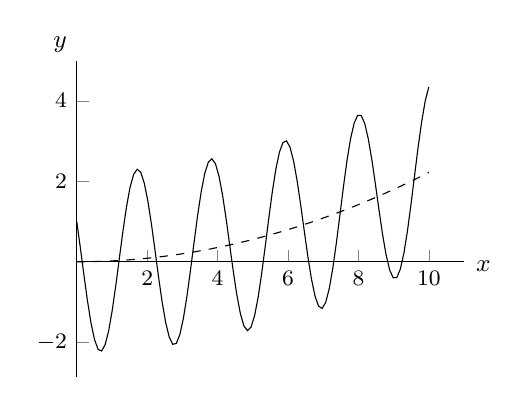
\begin{tikzpicture}
\begin{axis}[small,axis lines*=middle,xmin=0,xlabel={$x$},ylabel={$y$},ylabel style={rotate=-90},ylabel style ={at={(axis description cs:0,1.05)}},xlabel style={at={(axis description cs:1.05,0.4)}}]
\addplot[domain=0:10,samples=100]{407/405*cos(180/pi*3*x)-2*sin(180/pi*3*x)+x^2/45-2/405};
\addplot[dashed,domain=0:10]{x^2/45-2/405};
\end{axis}
\end{tikzpicture}
\caption{مثال \حوالہ{مثال_سادہ_دو_نا_معلوم_سر_الف} کا مخصوص حل۔}
\label{شکل_مثال_سادہ_دو_نا_معلوم_سر_الف}
\end{figure}
\انتہا{مثال}
%===================
\ابتدا{مثال}\شناخت{مثال_سادہ_دو_نا_معلوم_سر_ب}\quad ترمیمی قاعدے کا اطلاق\\
درج ذیل ابتدائی قیمت مسئلہ حل کریں۔
\begin{align*}
y''+2.4y'+1.44y=-5e^{-1.2x}, \quad y(0)=1, \quad y'(0)=0
\end{align*}

حل: پہلا قدم: متجانس مساوات کا حل:\quad متجانس مساوات کا امتیازی مساوات \عددی{\lambda^2+2.4\lambda+1.44=0} یعنی \عددی{(\lambda+1.2)^2=0} ہے جس کا دوہرا جذر \عددی{\lambda=-1.2} ہے جس سے \عددی{y_h=(c_1+c_2x)e^{-1.2x}} حاصل ہوتا ہے۔

دوسرا قدم: غیر متجانس مساوات کا حل:\quad تفرقی مساوات کے دائیں ہاتھ تفاعل \عددی{e^{-1.2x}} سے عام طور جدول \حوالہ{جدول_سادہ_دو_نا_معلوم_عددی_سر} کو دیکھ کر \عددی{y_p=Ce^{-1.2x}} لکھا جاتا البتہ ہم دیکھتے ہیں کہ یہ تفاعل متجانس مساوات کے امتیازی مساوات کے دوہرے جذر سے حاصل حل ہے۔یوں ترمیمی قاعدے کے تحت منتخب تفاعل کو \عددی{x^2} سے ضرب دینا ہو گا۔یوں درج ذیل چننا جائے گا
\begin{align*}
y_p=Cx^2e^{-1.2x}
\end{align*}
جس کے تفرقات \عددی{y'_p=(2x-1.2x^2)Ce^{-1.2x}} اور \عددی{y''_p=(1.44x^2-4.8x+2)Ce^{-1.2x}} ہیں۔ان تمام  کو غیر متجانس مساوات میں پر کرتے ہیں جہاں دونوں اطراف \عددی{e^{-1.2x}} کو حذف کیا گیا ہے۔
\begin{align*}
(1.44x^2-4.8x+2)C+2.4(2x-1.2x^2)C+1.44Cx^2=-5
\end{align*}
دونوں اطراف \عددی{x^2}، \عددی{x^1} اور \عددی{x^0} کے عددی سر برابر لکھے ہوئے \عددی{0=0}، \عددی{0=0} اور \عددی{2C=-5} لکھا جاتا ہے جس سے \عددی{C=-2.5} حاصل ہوتا ہے۔یوں \عددی{y_p=-2.5x^2e^{-1.2x}} حاصل ہوتا ہے لہٰذا عمومی حل درج ذیل ہو گا۔
 \begin{align*}
y=y_h+y_p=(c_1+c_2x)e^{-1.2x}-2.5x^2e^{-1.2x}
\end{align*}
تیسرا قدم: مخصوص حل:\quad ابتدائی معلومات \عددی{x=0}، \عددی{y(0)=1}  کو عمومی حل میں پر کرتے ہوئے \عددی{c_1=1} حاصل ہوتا ہے۔\عددی{y} کے تفرق
\begin{align*}
y'=[3x^2-(1.2c_2+5)x+c_2-1.2c_1]e^{-1.2x}
\end{align*} 
 میں \عددی{y'(0)=0} پر کرتے  ہوئے \عددی{0=2c_2-1.2c_1} یعنی \عددی{c_2=1.2} ملتا ہے۔یوں مخصوص حل درج ذیل لکھا جائے گا۔
\begin{align*}
y=(1+1.2x-2.5x^2)e^{-1.2x}
\end{align*}
مخصوص حل کو شکل \حوالہ{شکل_مثال_سادہ_دو_نا_معلوم_سر_ب} میں دکھایا گیا ہے۔
\begin{figure}
\centering
\begin{tikzpicture}
\begin{axis}[small,axis lines*=middle,xmin=0,xlabel={$x$},ylabel={$y$},ylabel style={rotate=-90},ylabel style ={at={(axis description cs:0,1.05)}},xlabel style={at={(axis description cs:1.05,0.4)}}]
\addplot[domain=0:8,samples=50]{(1+1.2*x-2.5*x^2)*e^(-1.2*x)};
\end{axis}
\end{tikzpicture}
\caption{مثال \حوالہ{مثال_سادہ_دو_نا_معلوم_سر_ب} کا مخصوص حل۔}
\label{شکل_مثال_سادہ_دو_نا_معلوم_سر_ب}
\end{figure}
\انتہا{مثال}
%======================
\ابتدا{مثال}\شناخت{مثال_سادہ_دو_نا_معلوم_سر_پ}\quad مجموعے کا قاعدہ\\
درج ذیل ابتدائی قیمت مسئلے کو حل کریں۔
\begin{align*}
y''3y'+2y=0.2\cos x+0.1x-0.4, \quad y(0)=-2.1, \quad y'(0)=3.2
\end{align*}

حل:پہلا قدم: متجانس مساوات کا حل:\quad متجانس مساوات \عددی{y''+3y'+2y=0} کا امتیازی مساوات \عددی{\lambda^2+3\lambda+2=0} یعنی \عددی{(\lambda+2)(\lambda+1)=0}  کے جذر \عددی{\lambda_1=-1} اور \عددی{\lambda_2=-2} ہیں جن سے  \عددی{y_h=c_1e^{-x}+c_2e^{-2x}} حاصل ہوتا ہے۔

دوسرا قدم: غیر متجانس مساوات کا حل:\quad غیر متجانس مساوات کے دائیں ہاتھ تفاعل کے تحت جدول \حوالہ{جدول_سادہ_دو_نا_معلوم_عددی_سر} سے
  \عددی{y_p=y_{p1}+y_{p2}} لکھتے ہیں جہاں 
\begin{align*}
y_{p1}=K\cos x+M\sin x, \quad y_{p2}=K_1x+K_0
\end{align*}
کے برابر ہیں۔یوں \عددی{y_p=K\cos x+M\sin x+K_1x+K_0} اور اس کے تفرقات 

\begin{align*}
y'_p=-K\sin x+M\cos x+K_1, \quad y''_p=-K\cos x-M\sin x
\end{align*}
کو غیر متجانس مساوات میں پر کرتے ہیں۔
\begin{multline*}
(-K\cos x-M\sin x)+3(-K\sin x+M\cos x+K_1)\\
+2(K\cos x+M\sin x+K_1x+K_0)=0.2\cos x+0.1x-0.4
\end{multline*}
دونوں اطراف \عددی{\cos x}، \عددی{\sin x}، \عددی{x^1} اور \عددی{x^0} کے عددی سر برابر لکھتے
\begin{align*}
-K+3M+2K=0.2, \quad -M-3K+2M=0, \quad 2K_1=0.1, \quad 3K_1+2K_0=-0.4
\end{align*}
ہوئے حل کرنے سے \عددی{K_0=-\tfrac{11}{40}}، \عددی{K_1=\tfrac{1}{20}}، \عددی{M=\tfrac{3}{50}} اور \عددی{K=\tfrac{1}{50}} ملتے ہیں لہٰذا 
\begin{align*}
y_p&=\tfrac{1}{50}\cos x+\tfrac{3}{50}\sin x+\tfrac{x}{20}-\frac{11}{40}
\end{align*}
لکھا جائے گا جس کو استعمال کرتے ہوئے عمومی حل
\begin{align*}
y&=y_h+y_p=c_1e^{-x}+c_2e^{-2x}+\tfrac{1}{50}\cos x+\tfrac{3}{50}\sin x+\tfrac{x}{20}-\frac{11}{40}
\end{align*}
حاصل ہوتا ہے۔

تیسرا قدم: مخصوص حل:\quad \عددی{y} اور \عددی{y'} میں ابتدائی معلومات پر کرتے ہوئے درج ذیل ہمزاد مساوات ملتے ہیں
\begin{align*}
c_1+c_2+\frac{1}{50}-\frac{11}{40}=-2.1,\quad -c_1-2c_2+\frac{3}{50}+\frac{1}{20}=3.2
\end{align*}
جنہیں حل کرتے ہوئے \عددی{c_1=-\tfrac{3}{5}} اور \عددی{c_2=-\tfrac{249}{200}} ملتے ہیں۔یوں مخصوص حل درج ذیل ہو گا۔
\begin{align*}
y=-\frac{3}{5}e^{-x}-\frac{249}{200}e^{-2x}+\tfrac{1}{50}\cos x+\tfrac{3}{50}\sin x+\tfrac{x}{20}-\frac{11}{40}
\end{align*}
مخصوص حل کو شکل \حوالہ{شکل_مثال_سادہ_دو_نا_معلوم_سر_پ} میں دکھایا گیا ہے۔
\begin{figure}
\centering
\begin{tikzpicture}
\begin{axis}[small,axis lines*=middle,xmin=0,xlabel={$x$},ylabel={$y$},ylabel style={rotate=-90},ylabel style ={at={(axis description cs:0,1.05)}},xlabel style={at={(axis description cs:1.05,0.7)}}]
\addplot[domain=0:20,samples=50]{1/50*cos(180/pi*x)+3/50*sin(180/pi*x)+x/20-11/40-249/200*e^(-2*x)-3/5*e^(-x)};
\end{axis}
\end{tikzpicture}
\caption{مثال \حوالہ{مثال_سادہ_دو_نا_معلوم_سر_پ} کا مخصوص حل۔}
\label{شکل_مثال_سادہ_دو_نا_معلوم_سر_پ}
\end{figure}
\انتہا{مثال}
%=====================

\جزوحصہء{توازن}
کسی بھی انجینئری نظام کا متوازن ہونا نہایت اہم ہوتا ہے۔مساوات  \حوالہ{مساوات_سادہ_دو_نا_معلوم_الف} کے مطابقتی متجانس مساوات کے امتیازی مساوات کے دونوں جذر منفی یا دونوں جذر کے حقیقی حصے منفی ہونے کی صورت میں نظام اور تفرقی مساوات کو \اصطلاح{متوازن}\فرہنگ{متوازن}\حاشیہب{stable}\فرہنگ{stable} کہتے ہیں۔ایسی صورت میں \عددی{t \to \infty} پر \عددی{y_h \to 0} ہو گا لہٰذا عارضی حل \عددی{y=y_h+y_p} آخر کار برقرار حل \عددی{y_p} کے قریب  قریب ہو گا۔ایسا نہ ہونے کی صورت میں نظام \اصطلاح{غیر متوازن}\فرہنگ{غیر متوازن}\حاشیہب{unstable}\فرہنگ{unstable} کہلاتا ہے۔چونکہ مثال \حوالہ{مثال_سادہ_دو_نا_معلوم_سر_الف} میں امتیازی مساوات کے جذر کے حقیقی حصے منفی مقدار نہیں ہیں لہٰذا یہ غیر متوازن نظام کو ظاہر کرتا ہے۔

اگلے دو حصوں میں ان مساوات کا استعمال ہو گا۔
%==============================

\حصہء{سوالات}


%==============================
سوال \حوالہ{سوال_سادہ_غیر_متجانس_مستقل_عددی_سر_الف} تا سوال \حوالہ{سوال_سادہ_غیر_متجانس_مستقل_عددی_سر_ب} میں دیے غیر متجانس خطی سادہ تفرقی مساوات کے حقیقی عمومی حل دریافت کریں۔

\ابتدا{سوال}\شناخت{سوال_سادہ_غیر_متجانس_مستقل_عددی_سر_الف}\quad
$y''-y'-6y=e^{-1.5x}$\\
جواب:\عددی{y=c_1e^{3x}+c_2e^{-2x}-\tfrac{4}{9}e^{-1.5x}}
\انتہا{سوال}
%===========================
\ابتدا{سوال}\quad
$y''+5y'+6y=e^{-3x}$\\
جواب:\عددی{y=c_1e^{-2x}+c_2e^{-3x}-(1+x)e^{-3x}}
\انتہا{سوال}
%===========================
\ابتدا{سوال}\quad
$4y''+12y'+9y=4^{-1.5x}$\\
جواب:\عددی{y=(c_1+c_2x)e^{-1.5x}+\tfrac{x^2}{2}e^{-1.5x}}
\انتہا{سوال}
%===========================
\ابتدا{سوال}\quad
$4y''+2y'+3y=4\cos 3x$\\
جواب:\عددی{y=c_1e^{-0.5x}+c_2e^{-1.5x}+\tfrac{32}{555}\sin 3x-\tfrac{44}{555}\cos 3x}
\انتہا{سوال}
%===========================
\ابتدا{سوال}\quad
$y''+4y=\sin 2x$\\
جواب:\عددی{y=c_1\sin 2x+c_2\cos 2x-0.5x\cos 2x}
\انتہا{سوال}
%===========================
\ابتدا{سوال}\quad
$9y''+4y=e^{-2x}\sin \frac{2x}{3}$\\
جواب:\عددی{y=c_1\cos\tfrac{2x}{3}+c_2\sin\tfrac{2x}{3}+\tfrac{e^{-2x}}{156}(2\cos\tfrac{2x}{3}+3\sin\tfrac{2x}{3})}
\انتہا{سوال}
%===========================
\ابتدا{سوال}\quad
$y''+3y'+2y=x^2$\\
جواب:\عددی{y=c_1e^{-x}+c_2e^{-2x}+\tfrac{2x^2-6x+7}{4}}
\انتہا{سوال}
%===========================
\ابتدا{سوال}\quad
$y''+9y=3\sin x+\sin 3x$\\
جواب:\عددی{y=c_1\cos 3x+c_2\sin 3x+\tfrac{3}{8}\sin x-\tfrac{x}{6}\cos 3x}
\انتہا{سوال}
%===========================
\ابتدا{سوال}\quad
$y''+8y'+15y=0.5x$\\
جواب:\عددی{y=c_1e^{-3x}+c_2e^{-5x}+\tfrac{15x-8}{450}}
\انتہا{سوال}
%===========================
\ابتدا{سوال}\شناخت{سوال_سادہ_غیر_متجانس_مستقل_عددی_سر_ب}\quad
$y''+2y'+y=x\cos x$\\
جواب:\عددی{y=(c_1+c_2x)e^{-x}+0.5\cos x+0.5(x-1)\sin x}
\انتہا{سوال}
%===========================
%===============================
سوال \حوالہ{سوال_سادہ_غیر_متجانس_مستقل_عددی_سر_پ} تا سوال \حوالہ{سوال_سادہ_غیر_متجانس_مستقل_عددی_سر_ت} غیر متجانس خطی سادہ تفرقی مساوات پر مبنی ابتدائی قیمت مسئلوں کے مخصوص حل حاصل کریں۔

%=========================
\ابتدا{سوال}\شناخت{سوال_سادہ_غیر_متجانس_مستقل_عددی_سر_پ}\quad
$y''+5y'+6y=0.2e^{-1.5x}, \quad y(0)=1.2,\quad y'(0)=-0.5$\\
جواب:\عددی{y=-\tfrac{4}{15}e^{-1.5x}+\tfrac{27}{10}e^{-2x}-\tfrac{53}{30}e^{-3x}}
\انتہا{سوال}
%================================
\ابتدا{سوال}\quad
$y''+2.7y'+1.8y=3.4e^{-1.2x}, \quad y(0)=-2,\quad y'(0)=-3$\\
جواب:\عددی{y=(\tfrac{102x-340}{9})e^{-1.2x}-20e^{-1.2x}+\tfrac{302}{9}e^{-1.5x}}
\انتہا{سوال}
%================================
\ابتدا{سوال}\quad
$y''+6y'+9y=1.1e^{-2x}, \quad y(0)=1,\quad y'(0)=-1$\\
جواب:\عددی{y=1.1e^{-2x}+(0.9x-0.1)e^{-3x}}
\انتہا{سوال}
%================================
\ابتدا{سوال}\quad
$y''+8y'+16y=0.7e^{-4x}, \quad y(0)=2,\quad y'(0)=-2$\\
جواب:\عددی{y=\tfrac{7}{20}x^2e^{-4x}+(6x+2)e^{-4x}}
\انتہا{سوال}
%================================
\ابتدا{سوال}\quad
$4y''+8y'+3y=24x^2, \quad y(0)=-2,\quad y'(0)=-2$\\
جواب:\عددی{y=-101e^{-0.5x}+\tfrac{59}{9}e^{-1.5x}+\tfrac{72x^2-384x+832}{9}}
\انتہا{سوال}
%================================
\ابتدا{سوال}\quad
$4y''+8y'+3y=2.4e^{-0.5x}+8x^2, \quad y(0)=3,\quad y'(0)=-2$\\
جواب:\عددی{y=(\tfrac{3x}{5}-\tfrac{301}{10})e^{-0.5x}+\tfrac{617}{270}e^{-1.5x}+\tfrac{8x^2}{3}-\tfrac{128x}{9}+\tfrac{832}{27}}
\انتہا{سوال}
%================================
\ابتدا{سوال}\quad
$6y''+29y'+35y=6\cos x, \quad y(0)=0.5,\quad y'(0)=-0.2$\\
جواب:\عددی{y=\tfrac{3}{29}\cos x+\tfrac{3}{29}\sin x+\tfrac{1197}{290}e^{-\tfrac{7}{3}x}-\tfrac{541}{145}e^{-\tfrac{5}{2}x}}
\انتہا{سوال}
%================================
\ابتدا{سوال}\quad
$y''+9y=\cos 3x, \quad y(0)=0.2,\quad y'(0)=0.3$\\
جواب:\عددی{y=\tfrac{1}{5}\cos 3x+(\tfrac{x}{6}+\tfrac{1}{10})\sin 3x}
\انتہا{سوال}
%================================
\ابتدا{سوال}\quad
$8y''-6y'+y=6\sinh x, \quad y(0)=0.2,\quad y'(0)=0.1$\\
جواب:\عددی{y=e^x-\tfrac{19}{5}e^{0.5x}+\tfrac{16}{5}e^{0.25x}-\tfrac{1}{5}e^{-x}}
\انتہا{سوال}
%================================
\ابتدا{سوال}\quad
$x^2y''-3xy'+3y=3\ln x-4, \quad y(1)=0,\,\, y'(1)=1,\,\, y_p=\ln x$\\
جواب:\عددی{y=\tfrac{1}{3}\ln x+\tfrac{4}{9}+\tfrac{5x^3}{9}-x}
\انتہا{سوال}
%================================
\ابتدا{سوال}\quad
$y''+2y'+10y=17\sin x-37\sin 3x, \quad y(0)=6.6,\quad y'(0)=-2.2$\\
جواب:\عددی{y=e^{-x}\cos 3x-\sin 3x+6\cos 3x+\tfrac{9}{5}\sin x-\tfrac{2}{5}\cos x}
\انتہا{سوال}
%================================
\ابتدا{سوال}\quad
$8y''-6y'+y=6\sinh x,\quad y(0)=0.2, \quad y'(0)=0.05$\\
جواب:\عددی{y=e^x-4e^{0.5x}+\tfrac{17}{5}e^{0.25x}-\tfrac{1}{5}e^{-x}}
\انتہا{سوال}
%===============================
\ابتدا{سوال}\شناخت{سوال_سادہ_غیر_متجانس_مستقل_عددی_سر_ت}\quad
$y''+4y'+4y=e^{-2x}\sin 2x,\quad y(0)=1, \quad y'(0)=-1.5$\\
جواب:\عددی{y=(1+x-0.25\sin 2x)e^{-2x}}
\انتہا{سوال}
%===============================
%===============================

\حصہ{جبری ارتعاش۔ گمک}\شناخت{حصہ_سادہ_دو_جبری_ارتعاش}
ہم اسپرنگ اور کمیت کے نظام پر حصہ \حوالہ{حصہ_سادہ_دو_قصری_نظام} میں غور کر چکے ہیں جہاں اس نظام کو متجانس خطی سادہ تفرقی مساوات
\begin{align}\label{مساوات_سادہ_دو_غیر_متجانس_نظام_الف}
my''+cy'+ky=0
\end{align}
سے ظاہر کیا گیا جہاں، ساکن حالت میں گیند کے مقام سے، حرکت کی صورت میں گیند کا فاصلہ \عددی{y(t)} سے ظاہر کیا جاتا ہے۔

حصہ \حوالہ{حصہ_سادہ_دو_قصری_نظام} میں نظام پر کوئی بیرونی قوت لاگو نہیں کیا گیا۔نظام کی حرکت صرف اور صرف نظام کی اندرونی قوتوں کی بنا تھی۔قوت جمود \عددی{my''}، قوت بحالی \عددی{ky} اور قوت روک \عددی{cy'} نظام کی اندرونی قوتیں تھیں۔   

آگے بڑھتے ہوئے اس نظام میں بیرونی قوت \عددی{r(t)} کا اضافہ کرتے ہیں۔شکل \حوالہ{شکل_سادہ_دو_درجی_اسپرنگ_کمیت_نظام_جبری} میں ایسا نظام دکھایا گیا ہے۔بیرونی قوت \عددی{r(t)} انتصابی سمت میں عمل کرتا ہے۔اس نظام کی نمونہ کشی درج ذیل تفرقی مساوات کرتی ہے۔
\begin{align}\label{مساوات_سادہ_دو_غیر_متجانس_نظام_ب}
my''+cy'+ky=r(t)
\end{align} 
میکانی طور پر اس مساوات کا مطلب ہے کہ ہر لمحہ \عددی{t} پر اندرونی قوتوں کا مجموعہ بیرونی قوت  \عددی{r(t)} کے برابر ہے۔اس نظام میں گیند کی حرکت کو \اصطلاح{جبری حرکت}\فرہنگ{حرکت!جبری}\فرہنگ{جبری!حرکت}\حاشیہب{forced motion}\فرہنگ{motion!forced} کہتے ہیں جبکہ بیرونی قوت کو \اصطلاح{جبری قوت}\فرہنگ{جبری!قوت}\فرہنگ{قوت!جبری}\حاشیہب{forcing function}\فرہنگ{function!forcing} یا \اصطلاح{داخلی قوت}\فرہنگ{داخلی!قوت}\فرہنگ{قوت!داخلی}\حاشیہب{input force}\فرہنگ{force!input}\فرہنگ{input!force} کہتے ہیں۔گیند کی حرکت کو نظام کا \اصطلاح{رد عمل}\فرہنگ{رد عمل}\حاشیہب{response}\فرہنگ{response} یا نظام کا \اصطلاح{ماحصل}\فرہنگ{ماحصل}\حاشیہب{output}\فرہنگ{output} بھی کہا جاتا ہے۔
\begin{figure}
\centering
\begin{tikzpicture}
\pgfmathsetmacro{\width}{0.9}
\pgfmathsetmacro{\height}{0.9}
\node[circle,fill=gray,inner sep=2.5mm] (b) at (0,0) {} ++(-0.37,0)node[left]{گیند} ++(0.74,0) node[right]{$m$};
\draw[decorate,decoration={coil,aspect=0.3, segment length=1.7mm, amplitude=3mm}] (0,3) -- (b)node[pos=0.5,shift={(-0.8,0)}]{اسپرنگ}node[pos=0.5,shift={(0.6,0)}]{$k$}; 
\fill [pattern = north east lines] (-1,3) rectangle (1,3.2);
\draw[thick] (-1,3) -- (1,3);
\draw[latex-latex] (1,0.6)--++(0,-1.2)node[pos=0.5,right]{$r(t)$};
%dashboard
\draw[] (b)--++(0,-0.8)coordinate(c);
\draw[ultra thick](c) ++(-\width/2+0.1,0)--++(\width-0.2,0);
\draw[thick] (c)++(-\width/2,\height/3)--++(0,-\height)--++(\width,0)--++(0,\height);
\draw(c)++(-\width/2,0)node[left]{\RL{روک (جاذب)}};
\draw(c)++(\width/2,0)node[right]{$c$};
\end{tikzpicture}
\caption{اسپرنگ اور کمیت کے نظام کی جبری ارتعاش۔}
\label{شکل_سادہ_دو_درجی_اسپرنگ_کمیت_نظام_جبری}
\end{figure}

ہمیں \اصطلاح{دوری}\فرہنگ{دوری!قوت}\فرہنگ{قوت!دوری}\حاشیہب{periodic}\فرہنگ{periodic!force}\فرہنگ{force!periodic} بیرونی قوتوں میں زیادہ دلچسپی ہے لہٰذا ہم
\begin{align*}
r(t)=F_0\cos \omega t\quad\quad (F_0 >0, \omega>0)
\end{align*}
طرز کے قوتوں پر توجہ دیں گے۔یوں غیر متجانس خطی سادہ تفرقی مساوات 
 \begin{align}\label{مساوات_سادہ_دو_غیر_متجانس_نظام_پ}
my''+cy'+ky=F_0 \cos \omega t
\end{align} 
حاصل ہوتی ہے جس کے حل سے بنیادی اہمیت کے حقائق حاصل ہوں گے  جن سے \اصطلاح{گمک}\فرہنگ{گمک}\حاشیہب{resonance}\فرہنگ{resonance} کی نمونہ کشی ممکن ہو گی۔
%======================

\جزوحصہء{غیر متجانس مساوات کا حل}
ہم نے حصہ \حوالہ{حصہ_سادہ_دو_غیر_متجانس} میں دیکھا کہ غیر متجانس مساوات \حوالہ{مساوات_سادہ_دو_غیر_متجانس_نظام_پ} کا عمومی حل  متجانس مساوات \حوالہ{مساوات_سادہ_دو_غیر_متجانس_نظام_الف} کے عمومی حل \عددی{y_h} اور مساوات \حوالہ{مساوات_سادہ_دو_غیر_متجانس_نظام_پ} کے کوئی بھی حل \عددی{y_p} کا مجموعہ ہے۔ہم \عددی{y_p} کو حصہ \حوالہ{حصہ_سادہ_دو_غیر_متجانس} کے نا معلوم عدد سر کی ترکیب سے حاصل کرتے ہیں۔یوں
\begin{align}\label{مساوات_سادہ_دو_جبری_تفاعل_حل}
y_p(t)=a \cos \omega t +b \sin \omega t
\end{align}
اور اس کے تفرقات
\begin{align*}
y'_p(t)=-\omega a \sin \omega t+\omega b \cos \omega t, \quad y''_p(t)=-\omega^2a\cos \omega t-\omega^2 b\sin \omega t
\end{align*}
کو مساوات \حوالہ{مساوات_سادہ_دو_غیر_متجانس_نظام_پ} میں پر کرتے ہوئے
 \begin{multline*}
m(-\omega^2a\cos \omega t-\omega^2 b\sin \omega t)+c(-\omega a \sin \omega t+\omega b \cos \omega t)\\
+k(a \cos \omega t+b \sin \omega t)=F_0 \cos \omega t
\end{multline*} 
 دونوں اطراف کے \عددی{\cos \omega t} کے عددی سر برابر لکھتے ہوئے اور دونوں اطراف \عددی{\sin \omega t} کے عددی سر برابر لکھتے ہوئے ہمزاد مساوات
\begin{align*}
(k-m\omega^2)a+c\omega b=F_0,\quad -c\omega a+(k-m\omega^2)b=0 
\end{align*}
حاصل ہوتے ہیں۔ان ہمزاد مساوات کو \عددی{a} اور \عددی{b} کے لئے حل کرتے ہیں۔\عددی{b} حذف کرنے کی خاطر بائیں مساوات کو \عددی{k-m\omega^2} سے ضرب دیتے ہوئے اور دائیں مساوات کو \عددی{-c\omega} سے ضرب دیتے ہوئے دونوں کا مجموعہ لیتے ہیں۔
\begin{align*}
(k-m\omega^2)^2a+c^2\omega^2a=F_0(k-m\omega^2)
\end{align*}
اسی طرح \عددی{a} حذف کرنے کی خاطر بائیں مساوات کو \عددی{c\omega} سے ضرب دیتے ہوئے اور دائیں مساوات کو \عددی{k-m\omega^2} سے ضرب دیتے ہوئے دونوں کا مجموعہ لیتے ہیں۔
\begin{align*}
c^2\omega^2 b+(k-m\omega^2)^2b=F_0c\omega
\end{align*}
ان مساوات میں جزو \عددی{c^2\omega^2+(k-m\omega^2)^2} صفر کے برابر نہیں ہے لہٰذا دونوں مساوات کو اس جزو سے تقسیم کیا جا سکتا ہے۔ایسا ہی کرتے ہوئے \عددی{a} اور \عددی{b} حاصل کرتے ہیں۔
\begin{align*}
a=F_0\frac{(k-m\omega^2)}{(k-m\omega^2)^2+c^2\omega^2}\, , \quad b=F_0\frac{c\omega}{(k-m\omega^2)^2+c^2\omega^2}
\end{align*}
اگر حصہ \حوالہ{حصہ_سادہ_دو_قصری_نظام} کی طرح \عددی{\sqrt{\tfrac{k}{m}}=\omega_0} لکھا جائے تب \عددی{k=m\omega_0^2} ہو گا اور 
\begin{align}\label{مساوات_سادہ_دو_نا_معلوم_عددی_سر_الف}
a=F_0\frac{m(\omega_0^2-\omega^2)}{m^2(\omega_0^2-\omega^2)^2+c^2\omega^2}\, , \quad b=F_0\frac{c\omega}{m^2(\omega_0^2-\omega^2)^2+c^2\omega^2}
\end{align}
ہوں گے۔

اس طرح غیر متجانس سادہ تفرقی مساوات \حوالہ{مساوات_سادہ_دو_غیر_متجانس_نظام_پ} کا عمومی حل
\begin{align}\label{مساوات_سادہ_دو_نا_معلوم_عددی_سر_ب}
y(t)=y_h(t)+y_p(t)
\end{align}
حاصل ہوتا ہے جہاں \عددی{y_h(t)} متجانس مساوات \حوالہ{مساوات_سادہ_دو_غیر_متجانس_نظام_الف} کا عمومی حل ہے اور \عددی{y_p(t)} مساوات \حوالہ{مساوات_سادہ_دو_جبری_تفاعل_حل} میں دیا گیا ہے جس میں \عددی{a} اور \عددی{b} کی قیمتیں مساوات \حوالہ{مساوات_سادہ_دو_نا_معلوم_عددی_سر_الف} سے پر کی گئی ہیں۔

آئیں اب اس میکانی نظام کی دو بالکل مختلف صورتوں پر غور کریں۔پہلی صورت \عددی{c=0} غیر قصری ہے جبکہ دوسری صورت \عددی{c>0} تقصیری ہے۔
%======================

\جزوحصہء{پہلی صورت:بلا تقصیر جبری ارتعاش۔ گمک}
اگر نظام میں قوت روک اتنا کم ہو کہ دورانیہ غور کے دوران اس کا اثر قابل نظر انداز ہو تب \عددی{c=0} لیا جا سکتا ہے۔یوں مساوات \حوالہ{مساوات_سادہ_دو_نا_معلوم_عددی_سر_الف} سے \عددی{a=\tfrac{F_0}{m(\omega_0^2-\omega^2)}} اور \عددی{b=0} حاصل ہوتے ہیں لہٰذا مساوات \حوالہ{مساوات_سادہ_دو_جبری_تفاعل_حل}
\begin{align}\label{مساوات_سادہ_دو_بلا_تقصیر_حل_الف}
y_p(t)=\frac{F_0}{m(\omega_0^2-\omega^2)}\cos \omega t=\frac{F_0}{k[1+\left(\frac{\omega}{\omega_0}\right)^2]}\cos \omega t
\end{align}
لکھا جائے گا جہاں \عددی{\omega_0^2=\tfrac{k}{m}} کا استعمال کیا گیا ہے۔یہاں ضروری ہے کہ \عددی{\omega \ne \omega_0} فرض کیا جائے جس کا مطلب ہے کہ جبری قوت کی تعدد \عددی{f=\tfrac{\omega}{2\pi}} بلا تقصیر نظام کی قدرتی تعدد \عددی{f_0=\tfrac{\omega_0}{2\pi}} سے مختلف فرض کی گئی ہے۔(بلا تقصیر نظام کی قدرتی تعدد کے لئے  مساوات \حوالہ{مساوات_سادہ_دو_درجی_اسپرنگ_کمیت_ارتعاش_الف} دیکھیں۔) یوں مساوات  \حوالہ{مساوات_سادہ_دو_بلا_تقصیر_حل_الف} اور مساوات \حوالہ{مساوات_سادہ_دو_درجی_اسپرنگ_کمیت_ارتعاش_ب} کی مدد سے بلا تقصیر نظام کی عمومی حل لکھتے ہیں۔

\begin{align}\label{مساوات_سادہ_دو_بلا_تقصیر_حل_ب}
y(t)=C\cos(\omega_0 t-\delta)+\frac{F_0}{m(\omega_0^2-\omega^2)}\cos \omega t
\end{align}
ہم دیکھتے ہیں کہ نظام کا رد عمل دو مختلف تعدد کے ہارمونی ارتعاش کا مجموعہ ہے۔
%============================================================

\جزوحصہء{گمک}
مساوات \حوالہ{مساوات_سادہ_دو_بلا_تقصیر_حل_الف} کا حیطہ
\begin{align}\label{مساوات_سادہ_دو_بلا_تقصیر_حل_پ}
a=\frac{F_0}{k} \rho, \quad \rho=\frac{1}{1-\left(\frac{\omega}{\omega_0}\right)^2}
\end{align}
\عددی{\omega} اور \عددی{\omega_0} پر منحصر ہے۔ \عددی{\omega \to \omega_0} کرنے سے \عددی{\rho \to \infty} اور \عددی{a \to \infty} ہو گا۔ داخلی جبری قوت کی تعدد کو نظام کی قدرتی تعدد کے برابر \عددی{(\omega=\omega_0)} کرنے سے انتہائی زیادہ حیطے کی پیدا ارتعاش  کو \اصطلاح{گمک}\فرہنگ{گمک}\حاشیہب{resonance}\فرہنگ{resonance} کہتے ہیں۔ \عددی{\rho} کو \اصطلاح{گمکی جزو}\فرہنگ{گمکی جزو}\حاشیہب{resonance factor}\فرہنگ{resonance!factor} کہتے ہیں جسے شکل \حوالہ{شکل_سادہ_دو_گمکی_جزو_بالمقابل_تعدد} میں دکھایا گیا ہے۔مساوات \حوالہ{مساوات_سادہ_دو_بلا_تقصیر_حل_پ} سے \عددی{\tfrac{\rho}{k}=\tfrac{a_0}{F_0}} لکھا جا سکتا ہے جو مخصوص حل \عددی{y_p} اور داخلی جبری قوت کے حیطوں کا تناسب ہے۔ہم جلد دیکھیں گے کہ ارتعاشی نظام میں گمک اہم کردار ادا کرتی ہے۔
\begin{figure}
\centering
\begin{tikzpicture}
\begin{axis}[small,axis lines*=middle,xmin=0,ymin=-4,ymax=4,xtick=\empty,ytick={1},xticklabels={$1$},xlabel={$\omega$},ylabel={$\rho$},xlabel style={at={(axis description cs:1.05,0.5)}},ylabel style={rotate=-90},ylabel style={at={(axis description cs:0,1.05)}}]
\addplot[domain=0:0.87]{1/(1-x^2)};
\addplot[domain=1.12:2.5]{1/(1-x^2)};
\addplot[dashed] plot coordinates {(1,-4) (1,4)}node[pos=0.4,fill=white]{$\omega_0$};
\end{axis}
\end{tikzpicture}
\caption{گمکی جزو \عددی{\rho(\omega)}}
\label{شکل_سادہ_دو_گمکی_جزو_بالمقابل_تعدد}
\end{figure}
گمک کی صورت میں غیر متجانس مساوات \حوالہ{مساوات_سادہ_دو_غیر_متجانس_نظام_پ} درج ذیل صورت اختیار کرتی ہے
 \begin{align}\label{مساوات_سادہ_دو_بلا_تقصیر_حل_ت}
y''+\omega_0^2 y=\frac{F_0}{m} \cos \omega t
\end{align} 
جس کا حل مساوات \حوالہ{مساوات_سادہ_دو_بلا_تقصیر_حل_الف} نہیں دیتی۔مساوات \حوالہ{مساوات_سادہ_دو_بلا_تقصیر_حل_ت} کا مخصوص حل \عددی{y_p}،  صفحہ \حوالہصفحہ{قاعدہ_سادہ_دو_ترمیمی_قاعدہ} پر دیے گئے ترمیمی قاعدہ کے تحت
\begin{align*}
y_p(t)=t(a\cos \omega_0 t +b\sin \omega_0 t)
\end{align*}
ہو گا جس کو مساوات \حوالہ{مساوات_سادہ_دو_بلا_تقصیر_حل_ت} میں پر کرتے ہوئے \عددی{a=0} اور \عددی{b=\tfrac{F_0}{2m\omega_0}} ملتے ہیں لہٰذا مخصوص حل
\begin{align}
y_p(t)=\frac{F_0}{2m\omega_0} t \sin \omega_0t
\end{align}
ہو گا جسے شکل \حوالہ{شکل_سادہ_دو_گمک_مخصوص_حل} میں دکھایا گیا ہے۔ہم دیکھتے ہیں کہ جزو \عددی{t} کی وجہ سے ارتعاش کا حیطہ مسلسل بڑھتا ہے۔عملاً اس کا مطلب ہے کہ کم قصری نظام زیادہ جھولے گا۔ نہایت کم تقصیر کی صورت میں نظام جھولنے سے تباہ ہو سکتا ہے۔
\begin{figure}
\centering
\begin{tikzpicture}
\begin{axis}[small,axis lines*=middle,xmin=0,xtick=\empty,ytick=\empty,xlabel={$t$},ylabel={$y_p$},xlabel style={at={(axis description cs:1.05,0.5)}},ylabel style={rotate=-90},ylabel style={at={(axis description cs:0,1.05)}}]
\addplot[domain=0:15,samples=100]{x*sin(180/pi*x)};
\addplot[dashed] plot coordinates {(0,0) (15,15)};
\addplot[dashed] plot coordinates {(0,0) (15,-15)};
\end{axis}
\end{tikzpicture}
\caption{گمک کی صورت میں مخصوص حل۔}
\label{شکل_سادہ_دو_گمک_مخصوص_حل}
\end{figure}
%===========================================================

\جزوحصہء{تھاپ}
\عددی{\omega} اور \عددی{\omega_0} قریب قریب ہونے کی صورت میں ایک دلچسپ صورت پیدا ہوتی ہے۔اسے سمجھنے کی خاطر مساوات \حوالہ{مساوات_سادہ_دو_بلا_تقصیر_حل_ب} میں \عددی{C=\tfrac{F_0}{m(\omega_0^2-\omega^2)}} اور \عددی{\delta=0} لکھتے ہیں۔
\begin{align}\label{مساوات_سادہ_دو_تھاپ_الف}
y(t)=\frac{F_0}{m(\omega_0^2-\omega^2)}(\cos \omega_0 t+\cos \omega t)\quad \quad (\omega \ne \omega_0)
\end{align}
اس کو ترتیب دیتے ہوئے
\begin{align}\label{مساوات_سادہ_دو_تھاپ_ب}
y(t)=\frac{2F_0}{m(\omega_0^2-\omega^2)}\sin\left( \frac{\omega_0+\omega}{2}t\right)\sin\left( \frac{\omega_0-\omega}{2}t\right)
\end{align}
لکھا جا سکتا ہے۔چونکہ \عددی{\omega_0} اور \عددی{\omega} نہایت قریب ہیں لہٰذا \عددی{\tfrac{\omega_0-\omega}{2}} چھوٹی مقدار ہو گی اور یوں دائیں سائن تفاعل کا دوری عرصہ زیادہ ہو گا۔اس کے برعکس \عددی{\tfrac{\omega_0+\omega}{2}} بڑی مقدار ہو گی لہٰذا بائیں سائن تفاعل کا دوری عرصہ کم ہو گا۔ شکل \حوالہ{شکل_سادہ_دو_گمک_تھاپ} میں اس مساوات کو دکھایا گیا ہے جہاں نقطہ دار لکیر دائیں سائن تفاعل کو ظاہر کرتی ہے۔اس شکل کے تفاعل کی آواز میں بلند تعدد کے ساتھ ساتھ کم تعدد بھی سنائی دیتی ہے جنہیں \اصطلاح{تھاپ}\فرہنگ{تھاپ}\حاشیہب{beats}\فرہنگ{beats} کہتے ہیں۔موسیقار  تھاپ پر دھیان دیتے ہوئے موسیقی آلے\فرہنگ{موسیقی!آلہ}\فرہنگ{آلہ!موسیقی}  کی تعدد درست کرتا ہے۔
\begin{figure}
\centering
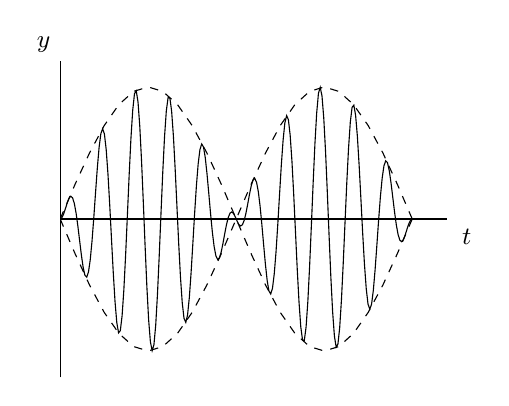
\begin{tikzpicture}
\begin{axis}[small,axis lines*=middle,xmin=0,xtick=\empty,ytick=\empty,xlabel={$t$},ylabel={$y$},xlabel style={at={(axis description cs:1.05,0.5)}},ylabel style={rotate=-90},ylabel style={at={(axis description cs:0,1.05)}}]
\addplot[domain=0:2*pi,samples=200]{sin(10.5*180/pi*x)*sin(180/pi*x)};
\addplot[dashed,domain=0:2*pi]{sin(180/pi*x)};
\addplot[dashed,domain=0:2*pi]{-sin(180/pi*x)};
\end{axis}
\end{tikzpicture}
\caption{قریبی سر تھاپ پیدا کرتے ہیں۔}
\label{شکل_سادہ_دو_گمک_تھاپ}
\end{figure}
%===========================

\جزوحصہء{دوسری صورت:قصری جبری ارتعاش}
اسپرنگ اور کمیت کے نظام میں قوت روک قابل نظر انداز نہ ہونے کی صورت میں \عددی{c > 0} ہو گا اور (جیسا ہم حصہ \حوالہ{حصہ_سادہ_اسپرنگ_کمیت} میں دیکھ چکے ہیں) متجانس مساوات \حوالہ{مساوات_سادہ_دو_غیر_متجانس_نظام_الف} کا حل \عددی{y_h} وقت گزرتے  گھٹے گا حتیٰ کہ \عددی{t \to \infty} پر \عددی{y_h \to 0} ہو گا۔عملاً کافی دیر بعد \عددی{y_h} صفر کے برابر ہو گا لہٰذا مساوات \حوالہ{مساوات_سادہ_دو_غیر_متجانس_نظام_پ} کا \اصطلاح{عارضی حل}\فرہنگ{عارضی حل}\فرہنگ{حل!عارضی}\حاشیہب{transient solution}\فرہنگ{transient!solution}  مساوات \حوالہ{مساوات_سادہ_دو_نا_معلوم_عددی_سر_ب} یعنی \عددی{y=y_h+y_p} آخر کار  \اصطلاح{برقرار حال حل}\فرہنگ{برقرار حال حل}\فرہنگ{حل!برقرار حال}\حاشیہب{steady state solution}\فرہنگ{steady state solution} \عددی{y_p} کے برابر ہو گا۔اس سے درج ذیل مسئلہ ثابت ہوتا ہے۔
%====================

\ابتدا{مسئلہ}\quad برقرار حال حل\\
سائن نما جبری قوت کی موجودگی میں قصری ارتعاشی نظام کافی دیر کے بعد عملاً ہارمونی ارتعاش کرے گا جس کی تعدد داخلی تعدد کے برابر ہو گی۔
\انتہا{مسئلہ}
%==============================

\جزوحصہ{برقرار حال حل کا حیطہ۔عملی گمک}
بلا تقصیر نظام میں  \عددی{\omega \to \omega_0} کرنے سے  \عددی{y_p} کا حیطہ لامتناہی ہو گا۔قصری نظام میں ایسا نہیں ہوتا اور \عددی{y_p} کا حیطہ محدود رہتا ہے۔ہاں کسی مخصوص \عددی{\omega} پر حیطہ زیادہ سے زیادہ ہو سکتا ہے جس کا دارومدار \عددی{c} کی قیمت پر ہو گا۔ایسی صورت کو \اصطلاح{عملی گمک}\فرہنگ{عملی گمک}\فرہنگ{گمک!عملی}\فرہنگ{resonance!practical} کہہ سکتے ہیں۔ عملی گمک اس لئے اہم ہے کہ اگر \عددی{c} کی قیمت زیادہ نہ ہو تب عین ممکن ہے کہ داخلی  جبری قوت نظام میں نقصان دہ یا  تباہ کن حیطے کی ارتعاش پیدا کر سکے۔جس زمانے میں انسان کو گمک کی سمجھ نہ تھی اس زمانے میں اس کو ایسے نقصان اٹھانے پڑتے تھے۔مشین، جہاز ، گاڑی، پل اور بلند عمارتیں وہ میکانی نظام ہیں جن میں ارتعاش پایا جاتا ہے۔زلزلہ یا آندھی بطور جبری قوت  بلند عمارت میں تباہ کن گمک پیدا کرتے ہوئے اسے ملبے کا ڈھیر بنا سکتی ہے۔بعض اوقات گمک سے پاک نظام کی تخلیق نا ممکن ہوتی ہے۔

\عددی{y_p} کا حیطہ بالمقابل \عددی{\omega} پر غور کی خاطر مساوات \حوالہ{مساوات_سادہ_دو_جبری_تفاعل_حل} کو درج ذیل صورت میں لکھتے ہیں
\begin{align}\label{مساوات_سادہ_دو_برقرار_عملی_گمک_الف}
y_p(t)=C^* \cos(\omega t-\eta)
\end{align}
جہاں
\begin{gather}
\begin{aligned}\label{مساوات_سادہ_دو_حیطہ_زاویہ_الف}
C^*(\omega)&=\sqrt{a^2+b^2}=\frac{F_0}{\sqrt{m^2(\omega_0^2-\omega^2)^2+c^2\omega^2}}\\
\eta(\omega)&=\tan^{-1}\frac{b}{a}=\tan^{-1}\frac{c\omega}{m(\omega_0^2-\omega^2)}
\end{aligned}
\end{gather}
ہیں۔انہیں شکل \حوالہ{شکل_سادہ_دو_حیطہ_زاویائی_فاصلہ} میں \عددی{c} کی مختلف قیمتوں کے لئے دکھایا گیا ہے۔\عددی{C^*} ردعمل \عددی{y_p} کا \اصطلاح{حیطہ}\فرہنگ{حیطہ}\حاشیہب{amplitude}\فرہنگ{amplitude} اور \عددی{\eta} اس کا \اصطلاح{زاویائی فاصلہ}\فرہنگ{زاویائی فاصلہ}\حاشیہب{phase angle}\فرہنگ{phase angle} ہے۔داخلی جبری تفاعل اور \عددی{y_p} میں زاویائی فرق \عددی{\eta} کے برابر ہو گا۔مثبت \عددی{\eta} کی صورت میں مساوات \حوالہ{مساوات_سادہ_دو_برقرار_عملی_گمک_الف} کے تحت داخلی قوت سے \عددی{y_p} \اصطلاح{پیچھے}\فرہنگ{پیچھے}\حاشیہب{lagging}\فرہنگ{lagging} ہے۔ 

حیطے کی زیادہ سے زیادہ قیمت دریافت کرنے کی خاطر \عددی{C^*} کے تفرق کو صفر کے برابر \عددی{(\tfrac{\dif C^*}{\dif \omega}=0)} پر کرتے ہیں۔
\begin{align*}
\frac{\dif C^*}{\dif \omega}=-\frac{F_0[2m^2(\omega_0^2-\omega^2)(-2\omega)+2c^2\omega]}{2[m^2(\omega_0^2-\omega^2)^2+c^2\omega^2]^{\frac{3}{2}}}=0
\end{align*}
کسر کا شمار کنندہ صفر ہونے کی صورت میں درج بالا صفر کے برابر ہو گا جس سے
\begin{align}
c^2=2m^2(\omega_0^2-\omega^2)\quad \quad (\omega_0^2=\frac{k}{m})
\end{align}
یعنی
\begin{align}\label{مساوات_سادہ_دو_عملی_گمک_تعدد_الف}
2m^2\omega^2=2m^2\omega_0^2-c^2=2mk-c^2
\end{align}
حاصل ہوتا ہے۔اس مساوات سے  \عددی{c^2 >2mk} کی صورت میں خیالی تعدد \عددی{\omega=\mp i\sqrt{\tfrac{c^2-2mk}{2m^2}}} حاصل ہوتا ہے۔خیالی تعدد حساب کے نقطہ نظر سے درست جواب  ہے لیکن عملی دنیا میں تعدد کی قیمت صرف حقیقی قیمت ممکن ہے۔ایسی صورت میں \عددی{\omega} کی قیمت بڑھانے سے \عددی{C^*} کی قیمت گھٹتی ہے۔اس کے برعکس \عددی{c^2<2mk} کی صورت میں  مساوات \حوالہ{مساوات_سادہ_دو_عملی_گمک_تعدد_الف} سے حقیقی تعدد \عددی{\omega_{\text{بلندتر}}}
\begin{align}\label{مساوات_سادہ_دو_عملی_گمک_تعدد_ب}
\omega^2_{\text{بلندتر}}=\omega_0^2-\frac{c^2}{2m^2}
\end{align}
حاصل ہوتی ہے۔مساوات \حوالہ{مساوات_سادہ_دو_عملی_گمک_تعدد_ب} سے ظاہر ہے کہ \عددی{c} کی قیمت کم کرنے سے \عددی{\omega_{\text{بلندتر}}} کی قیمت \عددی{\omega_0} بڑھتی ہے حتیٰ کہ \عددی{c \to 0} کی صورت میں \عددی{\omega_{\text{بلندتر}} \to 0} حاصل ہوتا ہے۔

\begin{figure}
\centering
\begin{subfigure}{0.5\textwidth}
\centering
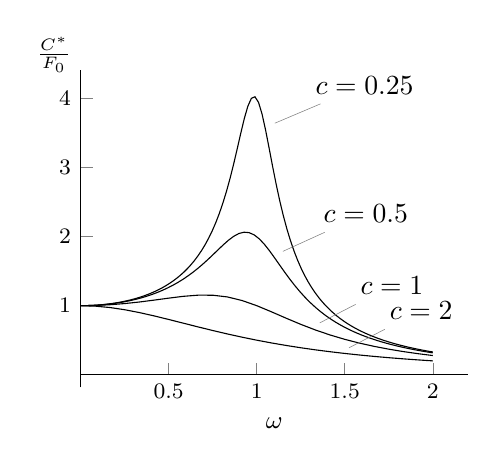
\begin{tikzpicture}
\begin{axis}[small,axis lines*=middle,xmin=0,xlabel={$\omega$},ylabel={$\frac{C^*}{F_0}$},ylabel style={rotate=-90},ylabel style={at={(axis description cs:0,1.05)}}]
\addplot[domain=0:2,samples=100]{1/sqrt((1-x^2)^2+x^2*0.25^2)}node[pos=0.52,pin=30:{$c=0.25$}]{};
\addplot[domain=0:2,samples=70]{1/sqrt((1-x^2)^2+x^2*0.5^2)}node[pos=0.52,pin=30:{$c=0.5$}]{};
\addplot[domain=0:2]{1/sqrt((1-x^2)^2+x^2*1^2)}node[pos=0.65,pin=30:{$c=1$}]{};
\addplot[domain=0:2]{1/sqrt((1-x^2)^2+x^2*2^2)}node[pos=0.75,pin=30:{$c=2$}]{};
\end{axis}
\end{tikzpicture}
\caption*{(الف) \عددی{k=1}، \عددی{m=1}، \عددی{\omega_0=1} رکھتے ہوئے\\ مختلف \عددی{c} کے لئے \عددی{\tfrac{C^*}{F_0}} بالمقابل \عددی{\omega}}
\end{subfigure}%
\begin{subfigure}{0.5\textwidth}
\centering
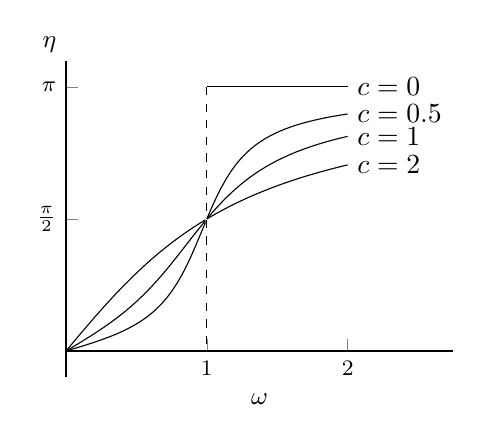
\begin{tikzpicture}
\begin{axis}[small,axis lines*=middle,xmin=0,xmax=2.75,xlabel={$\omega$},ylabel={$\eta$},ylabel style={rotate=-90},ylabel style={at={(axis description cs:0,1.05)}},ytick={1.571,3.142},yticklabels={$\frac{\pi}{2}$,$\pi$},xtick={1,2},xticklabels={$1$,$2$}]
\addplot[domain=0:0.99,samples=30]{rad(atan(0.5*x/(1-x^2)))};
\addplot[domain=1.001:2,samples=30]{pi+rad(atan(0.5*x/(1-x^2)))}node[right]{$c=0.5$};
%
\addplot[domain=0:0.99,samples=30]{rad(atan(1*x/(1-x^2)))};
\addplot[domain=1.001:2,samples=30]{pi+rad(atan(1*x/(1-x^2)))}node[right]{$c=1$};
%
\addplot[domain=0:0.99,samples=30]{rad(atan(2*x/(1-x^2)))};
\addplot[domain=1.001:2,samples=30]{pi+rad(atan(2*x/(1-x^2)))}node[right]{$c=2$};
%
\addplot[domain=0:0.99,samples=30]{rad(atan(0*x/(1-x^2)))};
\addplot[domain=1.001:2,samples=30]{pi+rad(atan(0*x/(1-x^2)))}node[right]{$c=0$};
%
\addplot[dashed] plot coordinates {(1,pi) (1,0)};
\end{axis}
\end{tikzpicture}
\caption*{(ب) \عددی{k=1}، \عددی{m=1}، \عددی{\omega_0=1} رکھتے ہوئے\\ مختلف \عددی{c} کے لئے \عددی{\eta} بالمقابل \عددی{\omega}}
\end{subfigure}%
\caption{مساوات \حوالہ{مساوات_سادہ_دو_حیطہ_زاویہ_الف} کا حیطہ اور زاویائی فاصلہ۔}
\label{شکل_سادہ_دو_حیطہ_زاویائی_فاصلہ}
\end{figure}

\عددی{\omega_{\text{بلندتر}}} کو مساوات \حوالہ{مساوات_سادہ_دو_حیطہ_زاویہ_الف} میں پر کرنے سے \عددی{C^*(\omega_{\text{بلندتر}})} حاصل کرتے ہیں۔
\begin{align}
C^*(\omega_{\text{بلندتر}})&=\frac{F_0}{\sqrt{m^2(\omega_0^2-\omega_0^2-\frac{c^2}{2m^2})^2+c^2(\omega_0^2-\frac{c^2}{2m^2})}}=\frac{2mF_0}{c\sqrt{4m^2\omega_0^2-c^2}}
\end{align}
آپ دیکھ سکتے ہیں کہ \عددی{c \to 0} کرنے سے \عددی{C^* \to \infty} حاصل ہو گا یعنی بلا تقصیر صورت میں لامتناہی حیطہ پایا جائے گا۔

%======================================

\حصہء{سوالات}
سوال \حوالہ{سوال_سادہ_دو_اسپرنگ_کمیت_الف} تا سوال \حوالہ{سوال_سادہ_دو_اسپرنگ_کمیت_ب} اسپرنگ اور کمیت کے نظام کی تفرقی مساوات ہیں۔ان کے برقرار حال حل دریافت کریں۔
%=======================================

\ابتدا{سوال}\شناخت{سوال_سادہ_دو_اسپرنگ_کمیت_الف}\quad
$y''+7y'+10y=4\cos 3t$\\
جواب:\عددی{y=\tfrac{2}{221}\cos 3t+\tfrac{42}{221}\sin 3t}
\انتہا{سوال}
%==================================
\ابتدا{سوال}\quad
$y''+4y'+3y=2\sin 6t$\\
جواب:\عددی{y=\tfrac{16}{555}\cos 6t-\tfrac{22}{555}\sin 6t}
\انتہا{سوال}
%==================================
\ابتدا{سوال}\quad
$10y''+11y'+3y=20+15\cos 3t-5\sin 2t$\\
جواب:\عددی{y=6.67+0.057\sin 3t-0.151\cos 3t+0.0998\sin 2t+0.059\cos 2t}
\انتہا{سوال}
%==================================
\ابتدا{سوال}\شناخت{سوال_سادہ_دو_اسپرنگ_کمیت_ب}\quad
$2y''+3y'+y=0.8+\sin 2t$\\
جواب:\عددی{y=0.8-0.08\sin 2t-0.07\cos 2t}
\انتہا{سوال}
%==================================
سوال \حوالہ{سوال_سادہ_دو_عارضی_حل_الف} تا سوال \حوالہ{سوال_سادہ_دو_عارضی_حل_ب} کے عارضی حل دریافت کریں۔

%===========================
\ابتدا{سوال}\شناخت{سوال_سادہ_دو_عارضی_حل_الف}\quad
$6y''+7y'+2y=3\sin (3.5t)$\\
جواب:\عددی{y=Ae^{-\tfrac{1}{2}t}=k-2e^{-\tfrac{2}{3}t}-0.037\sin (3.5t)-0.013\cos (3.5t)}
\انتہا{سوال}
%=======================
\ابتدا{سوال}\quad
$y''+2y'+2y=2\sin 2t$\\
جواب:\عددی{y=e^{-t}(A\cos t+B\sin 2t)-0.4\cos 2t-0.2\sin 2t}
\انتہا{سوال}
%=======================
\ابتدا{سوال}\quad
$y''+9y=4\cos 3t$\\
جواب:\عددی{y=A\cos 3t+B\sin 3t+\tfrac{2}{3}t\sin 3t+\tfrac{2}{9}\cos 3t}
\انتہا{سوال}
%=======================
\ابتدا{سوال}\quad
$y''+3y=\cos \sqrt{3}t-\sin \sqrt{3}t$\\
جواب:\عددی{y=A\cos \sqrt{3}t+B\sin\sqrt{3}t+\tfrac{t}{2\sqrt{3}}(\cos\sqrt{3}t+\sin\sqrt{3}t)+\tfrac{1}{6}\cos \sqrt{3}t}
\انتہا{سوال}
%=======================
\ابتدا{سوال}\quad
$y''+2y'+5y=3\cos 2t+2\sin 2t$\\
جواب:\عددی{y=e^{-t}(A\cos 2t+B\sin 2t)-\tfrac{10}{17}\cos 2t+\tfrac{11}{17}\sin 2t}
\انتہا{سوال}
%=======================
\ابتدا{سوال}\quad
$y''+y=5\sin \omega t \quad \quad (\omega^2 \ne 1)$\\
جواب:\عددی{y=A\cos \omega t+B\sin \omega t-\tfrac{5}{\omega^2-1}\sin\omega t}
\انتہا{سوال}
%=======================
\ابتدا{سوال}\quad
$y''+4y=3\cos 2t $\\
جواب:\عددی{y=A\cos 2t+B\sin 2t+\tfrac{3}{4}t\sin 2t+\tfrac{3}{8}\cos 2t}
\انتہا{سوال}
%=======================
\ابتدا{سوال}\quad
$y''+4y=e^{-2t}\cos 2t $\\
جواب:\عددی{y=A\cos 2t+B\sin 2t+\tfrac{e^{-2t}}{20}(\cos 2t-2\sin 2t)}
\انتہا{سوال}
%=======================
\ابتدا{سوال}\شناخت{سوال_سادہ_دو_عارضی_حل_ب}\quad
$y''+4y'+5y=2\cos t+3\sin t $\\
جواب:\عددی{y=e^{-2t}(A\cos t+B\sin t)-\tfrac{1}{8}\cos t+\tfrac{5}{8}\sin t}
\انتہا{سوال}
%=======================
سوال \حوالہ{سوال-سادہ_دو_ابتدائی_اسپرنگ_کمیت_الف} تا سوال \حوالہ{سوال-سادہ_دو_ابتدائی_اسپرنگ_کمیت_ب} ابتدائی قیمت مسئلے ہیں۔انہیں حل کریں۔

%=======================
\ابتدا{سوال}\شناخت{سوال-سادہ_دو_ابتدائی_اسپرنگ_کمیت_الف}\quad
$y''+4y=5\cos t,\quad y(0)=1,y'(0)=-1$\\
جواب:\عددی{y=\tfrac{5}{3}\cos t-\tfrac{1}{2}\sin 2t-\tfrac{2}{3}\cos 2t}
\انتہا{سوال}
%=====================
\ابتدا{سوال}\quad
$y''+9y=\sin t+\frac{1}{2}\sin 2t+\frac{1}{4}\sin 4t, \quad y(0)=0, \quad y'(0)=\frac{1}{5}$\\
جواب:\عددی{y=\tfrac{1}{8}\sin t+\tfrac{1}{10}\sin 2t+\tfrac{1}{168}\sin 3t-\tfrac{1}{28}\sin 4t}
\انتہا{سوال}
%=====================
\ابتدا{سوال}\quad
$y''+4y'+8y=4\cos( 0.5t), \quad y(0)=4, \quad y'(0)=-2$\\
جواب:\عددی{y=0.125\sin (0.5t)+0.484\cos (0.5t)+e^{-2t}[3.516\cos 2t+2.485\sin 2t]}
\انتہا{سوال}
%=====================
\ابتدا{سوال}\quad
$y''+4y'+5y=e^{-\frac{t}{2}}\cos \frac{t}{2}, \quad y(0)=0, \quad y'(0)=1$\\
جواب:\عددی{y=\tfrac{e^{-2t}}{15}(8\sin t-4\cos t)+\tfrac{e^{-0.5t}}{15}[4\cos (0.5t)+2\sin (0.5t)]}
\انتہا{سوال}
%=====================
\ابتدا{سوال}\quad
$y''+36y=\cos \pi t-\sin \pi t, \quad y(0)=0, \quad y'(0)=1$\\
جواب:\عددی{y=\tfrac{1}{\pi^2-36}(\sin\pi t-\cos \pi t+\cos 6t+\tfrac{\pi^2-\pi-36}{6}\sin 6t)}
\انتہا{سوال}
%=====================
\ابتدا{سوال}\شناخت{سوال-سادہ_دو_ابتدائی_اسپرنگ_کمیت_ب}\quad تھاپ \quad
$y''+36y=\cos (5.9t), \quad y(0)=1, \quad y'(0)=0$\\
جواب:\عددی{y=\tfrac{19}{119}\cos 6t+\tfrac{100}{119}\cos(5.9t)}
\انتہا{سوال}
%=====================
\ابتدا{سوال}\quad خود کار بندوق \\
\اصطلاح{خود کار بندوق}\فرہنگ{خود کار!بندوق}\فرہنگ{بندوق}\حاشیہب{automatic gun}\فرہنگ{gun} کے چلنے سے گولی پر نہایت کم دورانیے کے لئے  قوت عمل کرتا ہے اور اتنا ہی قوت بندوق کی نالی پر الٹ سمت میں عمل کرتا ہے۔نالی کا جھٹکا اسپرنگ برداشت کرتا ہے۔اس قوت کو تفاعل \عددی{1-\tfrac{t^2}{\pi^2}} سے ظاہر کرتے ہوئے درج ذیل تفرقی مساوات حل کریں جس میں \عددی{y(0)=0} اور \عددی{y'(0)=0} ہوں گے۔لمحہ \عددی{t=\pi} پر \عددی{y} اور \عددی{y'} دونوں استمراری ہیں۔
\begin{equation*}
y''+y=
\begin{cases}
1-\frac{t^2}{\pi^2} & 0 \le t \le \pi\\
0 & t<0, \, t>\pi
\end{cases}
\end{equation*}
جواب:\عددی{y=(1+\tfrac{2}{\pi^2})(1-\cos t)-\tfrac{t^2}{\pi^2}}
\انتہا{سوال}
%========================================

\حصہ{برقی ادوار کی نمونہ کشی}\شناخت{حصہ_سادہ_دو_برقی_ادوار}
شکل \حوالہ{شکل_سادہ_دو_سلسلہ_وار_دور_الف} میں  مزاحمت \عددی{R}، امالہ \عددی{L} اور \اصطلاح{برق گیر}\فرہنگ{برق گیر}\حاشیہب{capacitor}\فرہنگ{capacitor} \عددی{C}  کو منبع دباو کے ساتھ سلسلہ وار جوڑا گیا ہے۔اس دور کو سلسلہ وار\فرہنگ{سلسلہ وار دور}\فرہنگ{series circuit} \عددی{RLC} دور کہتے ہیں۔ہم صفحہ \حوالہصفحہ{مثال_سادہ_اول_برقی_دور_الف} پر مثال \حوالہ{مثال_سادہ_اول_برقی_دور_الف} میں مزاحمت اور امالہ کا سلسلہ وار \عددی{RL} دور دیکھ چکے ہیں جہاں مزاحمت پر دباو \عددی{v_R=IR} اور امالہ پر دباو \عددی{v_L=L\tfrac{\dif I}{\dif t}} کے مجموعے کو کرخوف کے قانون برائے دباو کے تحت درآیدہ دباو \عددی{E} کے برابر پر کیا گیا۔موجودہ \عددی{RLC} میں \عددی{v_R} اور \عددی{v_L} کے ساتھ برق گیر کا دباو \عددی{v_C} بھی جمع کیا جائے گا۔برق گیر پر دباو \عددی{v_C} اور اس میں ذخیرہ \اصطلاح{بار}\فرہنگ{بار}\حاشیہب{charge}\فرہنگ{charge} \عددی{Q} کا تعلق \عددی{Q=Cv_C} ہے۔ برق گیر کی اکائی \اصطلاح{فیراڈ}\فرہنگ{فیراڈ}\حاشیہب{Farad}\فرہنگ{Farad} \عددی{\si{\farad}} جبکہ بار کی اکائی \اصطلاح{کولمب}\فرہنگ{کولمب}\حاشیہب{Coulomb}\فرہنگ{Coulomb} \عددی{\si{\coulomb}} ہے ۔برقی بار اور برقی رو کا تعلق \عددی{Q=\int I \dif t} استعمال کرتے ہوئے برق گیر کے رو اور دباو کا تعلق 
\begin{align}
v_C=\frac{1}{C}\int I(t) \dif t
\end{align}
حاصل ہوتا ہے۔
\begin{figure}
\centering
\begin{tikzpicture}[american voltages]
\draw(0,0) to [american voltage source,l={${E(t)=E_0 \sin \omega t}$}]++(0,\y) to [resistor,l={$R$}]++(\x,0) to [inductor,l={$L$}]++(\x,0) to [capacitor,l={$C$}]++(0,-\y) to (0,0);
\end{tikzpicture}
\caption{مزاحمت، امالہ اور برق گیر سلسلہ وار منبع دباو کے ساتھ جڑے ہیں۔}
\label{شکل_سادہ_دو_سلسلہ_وار_دور_الف}
\end{figure}

یوں کرخوف مساوات دباو
\begin{align}\label{مساوات_سادہ_دو_سلسلہ_وار_الف}
LI'+RI+\frac{1}{C}\int I\dif t=E_0\sin \omega t\dif t
\end{align}
ہو گی جو تکمل و تفرقی مساوات ہے جس کا تفرق لیتے ہوئے تکمل سے پاک تفرقی مساوات
\begin{align}\label{مساوات_سادہ_دو_سلسلہ_وار_ب}
LI''+RI'+\frac{I}{C}=E'(t)=\omega E_0\cos \omega t
\end{align}
 حاصل ہوتی ہے۔یہ مستقل عددی سر والی غیر متجانس دو درجی سادہ تفرقی مساوات ہے جس کا حل \عددی{I(t)} دے گا۔مساوات \حوالہ{مساوات_سادہ_دو_سلسلہ_وار_الف} میں تکمل \عددی{Q} کے برابر ہے جبکہ  \عددی{I=\tfrac{\dif Q}{\dif t}} لکھا جا سکتا ہے جن سے درج ذیل مساوات حاصل ہوتی ہے جس کا حل \عددی{Q(t)} دے گا۔
\begin{align}\label{مساوات_سادہ_دو_سلسلہ_وار_پ}
LQ''+RQ'+\frac{Q}{C}=E(t)=E_0\sin \omega t
\end{align}
%===================

\جزوحصہء{سلسلہ وار دور میں رو کا حصول}
غیر متجانس تفرقی مساوات \حوالہ{مساوات_سادہ_دو_سلسلہ_وار_ب} کا حل \عددی{I=I_h+I_p} ہو گا جہاں \عددی{I_h} مطابقتی متجانس مساوات کا عمومی حل اور \عددی{I_p} غیر متجانس مساوات کا مخصوص حل ہے۔ہم \عددی{I_p} کو نا معلوم عددی سر کی ترکیب سے حاصل کرتے ہیں۔یوں مساوات \حوالہ{مساوات_سادہ_دو_سلسلہ_وار_ب} میں
\begin{gather}
\begin{aligned}
I_p&=a\cos \omega t+b\sin \omega t\\
I'_p&=-\omega a\sin \omega t+\omega b\cos \omega t\\
I''_p&=-\omega^2 a\cos \omega t-\omega^2 b\sin \omega t
\end{aligned}
\end{gather}
پر کرتے ہوئے دونوں اطراف \عددی{\cos \omega t} کے عددی سر برابر پر کرتے ہیں اور اسی طرح دونوں اطراف  \عددی{\sin \omega t} کے عددی سر برابر پر کرتے ہیں۔
\begin{align*}
\left(-\omega^2 L+\frac{1}{C}\right)a+\omega R b&=\omega E_0\\
-\omega R a+\left(-\omega^2 L+\frac{1}{C}\right)b&=0
\end{align*}
ان مساوات کو \عددی{\omega} سے تقسیم کرتے ہوئے 
\begin{align}
S=\omega L-\tfrac{1}{\omega C}
\end{align}
 لکھتے ہیں جہاں \عددی{S} کو \اصطلاح{متعاملیت}\فرہنگ{متعاملیت}\حاشیہب{reactance}\فرہنگ{reactance} کہتے ہیں۔یوں درج ذیل ہمزاد مساوات ملتے ہیں۔
\begin{align*}
-S a+R b&=E_0\\
-R a-S b&=0
\end{align*}
\عددی{b} حذف کرنے کی خاطر پہلی مساوات کو \عددی{S} اور دوسری کو \عددی{R} سے ضرب دیتے ہوئے ان کا مجموعہ لیتے ہیں۔\عددی{a} حذف کرنے کی خاطر پہلی مساوات کو \عددی{R} اور دوسری کو \عددی{-S} سے ضرب دیتے ہوئے ان کا مجموعہ لیتے ہیں۔
\begin{align}
-(S^2+R^2)a=E_0S,\quad (R^2+S^2)b=E_0 R
\end{align}
ان سے درج ذیل عددی سر حاصل ہوتے ہیں
 \begin{align}
a=-\frac{E_0S}{S^2+R^2}\, ,\quad b=\frac{E_0 R}{S^2+R^2}
\end{align}
جنہیں استعمال کرتے ہوئے \عددی{I_p} لکھتے ہیں۔
\begin{align}
I_p(t)=-\frac{E_0S}{S^2+R^2}\cos \omega t+\frac{E_0 R}{S^2+R^2} \sin \omega t
\end{align}
اس کو 
\begin{align}
I_p(t)=I_0\sin(\omega t-\theta)
\end{align}
بھی لکھا جا سکتا ہے جہاں
\begin{align}
I_0=\sqrt{a^2+b^2}=\frac{E_0}{\sqrt{S^2+R^2}}\, , \quad \tan \theta=-\frac{a}{b}=\frac{S}{R}
\end{align}
ہیں۔\عددی{I_0} کو رو کا حیطہ اور \عددی{\theta} کو رو کا زاویہ کہتے ہیں۔داخلی دباو سے رو \عددی{\theta} زاویے کے فاصلے پر ہے۔درج بالا مساوات میں \عددی{\tfrac{E_0}{I_0}=\sqrt{S^2+R^2}} لکھا جا سکتا ہے  جو قانون اوہم سے مشابہت رکھتا ہے لہٰذا \عددی{\sqrt{S^2+R^2}} کو \اصطلاح{برقی رکاوٹ}\فرہنگ{برقی رکاوٹ}\حاشیہب{impedance}\فرہنگ{impedance} کہا جاتا ہے۔

مساوات \حوالہ{مساوات_سادہ_دو_سلسلہ_وار_ب} کے مطابقتی متجانس مساوات کی امتیازی مساوات
\begin{align*}
\lambda^2+\frac{R}{L}\lambda+\frac{1}{LC}=0
\end{align*}
کے جذر
\begin{align*}
\lambda=-\frac{R}{2L}\mp \sqrt{\frac{R^2}{4L^2}-\frac{1}{LC}}
\end{align*}
ہیں جن میں \عددی{\alpha=\tfrac{R}{2L}} اور \عددی{\beta=\sqrt{\tfrac{R^2}{4L^2}-\tfrac{1}{LC}}} لکھتے ہوئے
\begin{align*}
\lambda_1=-\alpha+\beta, \quad \lambda_2=-\alpha-\beta
\end{align*}
لکھا جا سکتا ہے۔یوں \عددی{I_h} درج ذیل ہو گا۔
\begin{align*}
I_h(t)=c_1e^{\lambda_1 t}+c_2 e^{\lambda_2 t}
\end{align*}
کسی بھی حقیقی دور میں \عددی{R} کبھی بھی صفر کے برابر نہیں ہوتا۔یوں \عددی{R>0} اور \عددی{\alpha>0} ہوں گے۔اس طرح \عددی{t \to \infty} پر \عددی{I_h \to 0} ہو گا لہٰذا \عددی{RLC} دور کا عمومی حل آخر کار \عددی{I_p} کے برابر ہو گا جو داخلی دباو کے تعدد \عددی{\omega} پر ہارمونی ارتعاش کرتی رو کو ظاہر کرتی ہے۔ 
%=======================

\ابتدا{مثال}\شناخت{مثال_سادہ_دو_سلسلہ_وار_دور_الف}
سلسلہ وار \عددی{RLC} دور میں سو اوہم کی مزاحمت \عددی{R=\SI{100}{\ohm}}، آدھا ہینری امالہ  \عددی{L=\SI{0.5}{\henry}}، بیس ملی فیراڈ برق گیر
  \عددی{C=\SI{20}{\milli\farad}} اور داخلی دباو \عددی{E(t)=310\sin (2\pi 50 t)} وولٹ  ہیں۔لمحہ \عددی{t=0} پر رو اور برق گیر میں ذخیرہ بار صفر کے برابر ہیں۔دور میں رو \عددی{I(t)} حاصل کریں۔

حل:مساوات \حوالہ{مساوات_سادہ_دو_سلسلہ_وار_ب} میں دی گئی معلومات پر کرتے ہوئے
\begin{align*}
0.5I''+100I'+50I=(100\pi) (310)\cos (100\pi t)
\end{align*}
ملتا ہے جس سے متجانس مساوات \عددی{0.5I''+100I'+50I=0} لکھ کر امتیازی مساوات حاصل کرتے ہیں۔
\begin{align*}
0.5\lambda^2+100\lambda+50=0
\end{align*}
امتیازی مساوات کے جذر \عددی{\lambda_1=-199.5} اور \عددی{\lambda_2=-0.5} ہیں لہٰذا
\begin{align*}
I_h(t)=c_1e^{-199.5t}+c_2e^{-0.5t}
\end{align*}
ہو گا۔آپ دیکھ سکتے ہیں کہ \عددی{I_h} بہت جلد صفر کے برابر ہو گا۔

دور کی متعاملیت \عددی{S=100\pi0.5-\tfrac{1}{100\pi0.02}=156.92} لیتے ہوئے 
\begin{align*}
I_p(t)=a\cos (100\pi t)+b\sin (100\pi t)
\end{align*}
کے مستقل حاصل کرتے ہیں۔
\begin{align*}
a=-\frac{310\times 156.92}{156.92^2+100^2}=-1.4049, \quad b=\frac{310\times 100}{156.92^2+100^2}=0.8953
\end{align*}
یوں 
\begin{align}
I_p(t)=-1.4049\cos (100\pi t)+0.8953\sin (100\pi t)=1.422\sin(100\pi t-1.003)
\end{align}
ہو گا لہٰذا عمومی حل
\begin{align*}
I(t)=I_h+I_p=c_1e^{-199.5t}+c_2e^{-0.5t}+1.422\sin(100\pi t-1.003)
\end{align*}
ہو گا۔ابتدائی معلومات کو استعمال کرتے ہوئے \عددی{c_1} اور \عددی{c_2} دریافت کرتے ہیں۔عمومی حل میں \عددی{t=0} پر \عددی{I(0)=0} پر کرنے سے 
\begin{align}\label{مساوات_سادہ_دو_متجانس_حل_کا_سر_الف}
c_1+c_2-1.4049=0, \implies c_1=1.4049-c_2
\end{align}
ملتا ہے۔مساوات \حوالہ{مساوات_سادہ_دو_سلسلہ_وار_الف} میں تکمل کی قیمت بار کے برابر ہے یعنی \عددی{\int I \dif t=Q} لہٰذا \عددی{t=0} پر ابتدائی معلومات \عددی{Q(0)=0} اور \عددی{I(0)=0} استعمال کرتے ہوئے مساوات \حوالہ{مساوات_سادہ_دو_سلسلہ_وار_الف} سے
\begin{align*}
LI'(0)+RI(0)=E_0\sin 0 \quad \implies I'=0
\end{align*}
حاصل ہوتا ہے۔عمومی حل کے تفرق میں \عددی{I'(0)=0} پر کرنے سے
\begin{align*}
I'(0)=-199.5c_1-0.5c_2+0.8953(2\pi 50)=0
\end{align*}
حاصل ہوتا ہے جس کو مساوات \حوالہ{مساوات_سادہ_دو_متجانس_حل_کا_سر_الف} کی مدد سے حل کرتے ہوئے \عددی{c_1=1.4099} اور \عددی{c_2=-0.00497} ملتے ہیں۔یوں مخصوص حل یعنی دور میں رو درج ذیل ہو گی۔
\begin{align*}
I(t)=1.4099e^{-199.5t}-0.00497e^{-0.5t}+1.422\sin(100\pi t-1.003)
\end{align*}
شکل \حوالہ{شکل_مثال_سادہ_دو_سلسلہ_وار_دور_الف}-الف میں \عددی{I(t)} کو نقطہ دار لکیر جبکہ \عددی{I_p} کو ٹھوس لکیر سے ظاہر کیا گیا ہے۔چونکہ \عددی{I_h} بہت جلد صفر کے برابر ہو جاتا ہے لہٰذا \عددی{I} اور \عددی{I_p} میں صرف شروع میں فرق پایا جاتا ہے۔شکل-ب میں \عددی{E(t)} اور \عددی{I_p(t)} کو دکھایا گیا ہے۔ان دونوں میں زاویائی فاصلہ \عددی{1.003} ریڈیئن یعنی \عددی{57.5^{\circ}} ہے جو شکل میں صاف واضح ہے۔ہم کہتے ہیں کہ دباو سے رو \عددی{57.5^{\circ}} \اصطلاح{پیچھے}\فرہنگ{پیچھے}\حاشیہب{lagging}\فرہنگ{lagging} ہے۔آپ یہاں خود تسلی کر سکتے ہیں کہ \عددی{\omega L > \tfrac{1}{\omega C}} کی صورت میں داخلی دباو سے رو \اصطلاح{پیچھے} ہو گی جبکہ  \عددی{\omega L < \tfrac{1}{\omega C}} کی صورت میں داخلی دباو سے رو \اصطلاح{آگے} ہو گی۔  \عددی{\omega L = \tfrac{1}{\omega C}} کی صورت میں داخلی دباو اور رو \اصطلاح{ہم زاویہ}\فرہنگ{ہم زاویہ}\حاشیہب{in-phase}\فرہنگ{in-phase} ہوں گے یعنی ان میں زاویائی فاصلہ نہیں پایا جاتا۔
\begin{figure}
\centering
\begin{subfigure}{0.5\textwidth}
\centering
\begin{tikzpicture}
\begin{axis}[small,xmin=0,axis lines*=middle,xlabel={$t$},ylabel={$I(t)$},ylabel style={rotate=-90},ylabel style={at={(axis description cs:0,1.05)}},xtick=\empty,ytick=\empty,xlabel style={at={(axis description cs:1.05,0.45)}}]
\addplot[dashed,domain=0:0.04,samples=100]{1.4*e^(-199.5*x)-0.00497*e^(-0.5*x)-1.4049*cos(180/pi*100*pi*x)+0.8953*sin(180/pi*100*pi*x)};
\addplot[domain=0:0.04,samples=100]{-1.4049*cos(180/pi*100*pi*x)+0.8953*sin(180/pi*100*pi*x)};
\end{axis}
\end{tikzpicture}
\caption*{(الف) قصری دور میں عمومی حل آخر کار \عددی{I_p} کے برابر ہو گا۔}
\end{subfigure}%
\begin{subfigure}{0.5\textwidth}
\centering
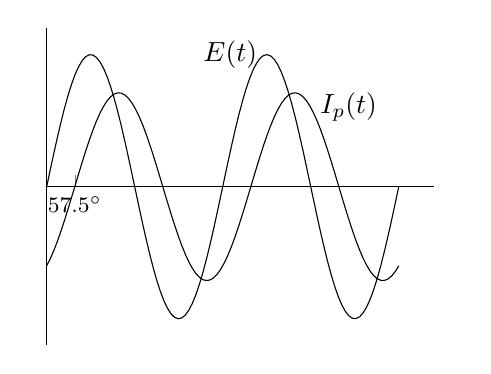
\begin{tikzpicture}
\begin{axis}[small,axis lines*=middle,xlabel=\empty,ylabel=\empty,xtick={0.0032},xticklabels={$57.5^{\circ}$},ytick=\empty,xlabel style={at={(axis description cs:1.05,0.45)}},scaled x ticks=false,xmin=0]
\addplot[domain=0:0.04,samples=100]{2*sin(180/pi*100*pi*x)}node[pos=0.625,left]{$E(t)$};
\addplot[domain=0:0.04,samples=100]{1.422*sin(180/pi*100*pi*x-57.48)}node[pos=0.75,right]{$I_p(t)$};
\end{axis}
\end{tikzpicture}
\caption*{(ب) دباو سے رو پیچھے ہے۔}
\end{subfigure}%
\caption{مثال \حوالہ{مثال_سادہ_دو_سلسلہ_وار_دور_الف} کی رو کے خطوط۔}
\label{شکل_مثال_سادہ_دو_سلسلہ_وار_دور_الف}
\end{figure}
\انتہا{مثال}
%=================================

\جزوحصہء{برقی اور میکانی مقدار کی مماثلت}
دو بالکل مختلف نظام کی ایک ہی تفرقی مساوات ہو سکتی ہے۔اسپرنگ اور کمیت کی تفرقی مساوات \حوالہ{مساوات_سادہ_دو_غیر_متجانس_نظام_پ} اور سلسلہ وار \عددی{RLC} کی مساوات \حوالہ{مساوات_سادہ_دو_سلسلہ_وار_ب} کو یہاں موازنے کے لئے دوبارہ پیش کرتے ہیں۔ 
 \begin{align*}
my''+cy'+ky=F_0 \cos \omega t, \quad LI''+RI'+\frac{I}{C}=E'(t)=\omega E_0\cos \omega t
\end{align*} 
آپ دیکھ سکتے ہیں کہ میکانی نظام میں کمیت اور برقی نظام  میں امالہ تفرقی مساوات میں یکساں کردار ادا کرتے ہیں۔کمیت کی جمود کی طرح  امالہ برقی دور کی رو میں تبدیلی کو روکنے کی کوشش کرتی ہے۔اسی طرح \عددی{c} اور \عددی{R} تفرقی مساوات میں یکساں کردار ادا کرتے ہیں اور نظام میں توانائی کی ضیاع کا باعث بنتے ہیں۔ اسپرنگ کا مستقل \عددی{k} اور  برق گیر کا بالعکس متناسب \عددی{\tfrac{1}{C}} یکساں کردار ادا کرتے ہیں۔میکانی جبری قوت \عددی{F_0\cos \omega t} اور برقی داخلی دباو کا تفرق \عددی{\omega E_0\cos \omega t} یکساں کردار ادا کرتے ہیں۔میکانی اور برقی نظام کی یکسانیت کو جدول \حوالہ{جدول_سادہ_دو_میکانی_برقی_یکسانیت} میں پیش کیا گیا ہے۔
\begin{table}
\caption{میکانی اور برقی نظام میں یکساں عناصر۔}
\label{جدول_سادہ_دو_میکانی_برقی_یکسانیت}
\centering
\begin{tabular}{rr}
برقی نظام & میکانی نظام\\
\hline
امالہ \عددی{L} & کمیت \عددی{m} \\
مزاحمت \عددی{R} & قصری مستقل \عددی{c}\\
برق گیر کا بالعکس \عددی{\tfrac{1}{C}} & اسپرنگ مستقلہ \عددی{k}\\
داخلی دباو کا تفرق \عددی{\omega E_0\cos \omega t} & جبری قوت \عددی{F_0\cos \omega t}\\
برقی رو \عددی{I(t)} & ہٹاو \عددی{y(t)}
\end{tabular}
\end{table}

میکانی اور برقی نظام میں یکسانیت صحیح معنوں میں صرف مقداری نوعیت کی ہے۔یوں ہم میکانی نظام کے مطابق ایسا برقی دور تخلیق دے سکتے ہیں جس میں رو بالمقابل وقت میکانی نظام میں ہٹاو بالمقابل وقت کے بالکل برابر ہو گی۔یہ ایک انتہائی اہم نتیجہ ہے کیونکہ میکانی نظام مثلاً پل یا بلند عمارت کا برقی نمونہ انتہائی آسانی اور سستے دام بناتے ہوئے اس کی کارکردگی پر تفصیلاً  غور کیا جا سکتا ہے۔ مزید، برقی متغیرات مثلاً رو یا دباو انتہائی آسانی سے ٹھیک ٹھیک ناپے جا سکتے ہیں جبکہ میکانی متغیرات اتنے آسانی سے اور ٹھیک ٹھیک ناپنا اتنا آسان ثابت نہیں ہوتا۔

میکانی متغیرات کو برقی متغیرات میں تبدیل کرنے والے کئی \اصطلاح{مبدل}\فرہنگ{مبدل}\حاشیہب{transducer}\فرہنگ{transducer} اسی مشابہت پر کام کرتے ہیں۔  
%====================================
%===================================

\حصہء{سوالات}
سوال \حوالہ{سوال_سادہ_دو_سلسلہ_وار_خصوصی_الف} تا سوال \حوالہ{سوال_سادہ_دو_سلسلہ_وار_خصوصی_ب} خصوصی  سلسلہ وار \عددی{RLC}  ادوار ہیں۔

%==============
\ابتدا{سوال}\شناخت{سوال_سادہ_دو_سلسلہ_وار_خصوصی_الف}
سلسلہ وار \عددی{RC} دور شکل \حوالہ{شکل_سادہ_دو_سلسلہ_وار_مزاحمت_برق_گیر}-الف میں دکھایا گیا ہے جہاں داخلی دباو مستقل مقدار \عددی{E(t)=E_0} ہے۔دور کی نمونہ کشی کرتے ہوئے برقی رو دریافت کریں۔
\begin{figure}
\centering
\begin{subfigure}{0.5\textwidth}
\centering
\begin{tikzpicture}
\draw(0,0) to [american voltage source,l={$E(t)$}]++(0,\y) to [resistor,l={$R$}]++(\x,0) to [capacitor,l={$C$}]++(0,-\y) to [short](0,0);
\end{tikzpicture}
\caption*{(الف) سلسلہ وار \عددی{RC} دور۔}
\end{subfigure}%
\begin{subfigure}{0.5\textwidth}
\centering
\begin{tikzpicture}
\begin{axis}[small,axis lines*=middle,xmin=0,xlabel={$t$},ylabel={$I(t)$},ylabel style={rotate=-90},ylabel style={at={(axis description cs:0,1.05)}},ytick={1},yticklabels={$c$},xtick=\empty]
\addplot[domain=0:4]{e^(-x)};
\end{axis}
\end{tikzpicture}
\caption*{سلسلہ وار \عددی{RC} کی رو بالمقابل وقت۔}
\end{subfigure}%
\caption{سلسلہ وار \عددی{RC} دور اور اس کی رو۔}
\label{شکل_سادہ_دو_سلسلہ_وار_مزاحمت_برق_گیر}
\end{figure} 

جوابات:\عددی{RI'+\tfrac{I}{C}=0}، رو \عددی{I=ce^{-\tfrac{t}{RC}}} کو شکل \حوالہ{شکل_سادہ_دو_سلسلہ_وار_مزاحمت_برق_گیر}-ب میں دکھایا گیا ہے۔
\انتہا{سوال}
%======================
\ابتدا{سوال}
شکل \حوالہ{شکل_سادہ_دو_سلسلہ_وار_مزاحمت_برق_گیر}-الف کو سائن نما برقی دباو \عددی{E(t)=E_0\sin \omega t} کے لئے حل کریں۔

جواب:\عددی{RI'+\tfrac{I}{C}=\omega E_0\cos \omega t}، 
\عددی{I=ce^{-\tfrac{t}{RC}}+\tfrac{\omega C E_0}{1+\omega^2 R^2 C^2}(\cos \omega t+\omega RC \sin \omega t)}
\انتہا{سوال}
%=============================
\ابتدا{سوال}
شکل \حوالہ{شکل_سادہ_دو_سلسلہ_وار_مزاحمت_برق_گیر}-الف میں \عددی{R=\SI{50}{\ohm}}، \عددی{C=\SI{0.25}{\milli\farad}} اور 
\عددی{E(t)=20\sin 100 t} لیتے ہوئے برقرار حال رو دریافت کریں۔دباو کو حوالہ لیتے ہوئے برقرار حل رو کا زاویہ کتنا ہے؟ \عددی{E(t)} اور \عددی{I(t)} کے خط اکٹھے کھینچیں۔

\begin{figure}
\centering
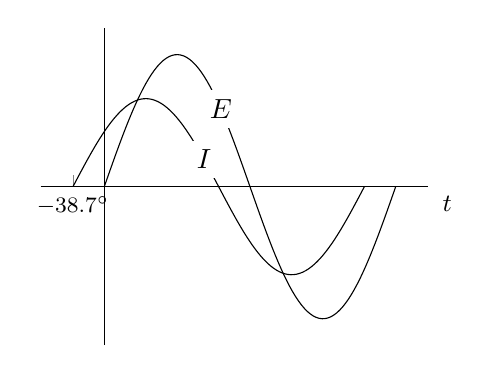
\begin{tikzpicture}
\begin{axis}[small,axis lines*=middle,xlabel={$t$},xlabel style={at={(axis description cs:1.05,0.5)}},ylabel=\empty,ylabel style={rotate=-90},ytick=\empty,xtick={-38.7},xticklabels={$-38.7^{\circ}$}]
\addplot[domain=0:360,samples=100]{1.5*sin(x)}node[pos=0.4,fill=white]{$E$};
\addplot[domain=-38.7:321.3,samples=100]{sin(x+38.7)}node[pos=0.45,fill=white]{$I$};
\end{axis}
\end{tikzpicture}
\caption{\عددی{RC} دور میں دباو سے برقرار رو آگے رہتی ہے۔}
\label{شکل_سوال_مزاحمتی_برق_گیر_آگے}
\end{figure}%

جواب:\عددی{I_p=\tfrac{2}{\sqrt{41}}\sin(100t+0.6747)}؛ دباو سے رو \عددی{38.7^{\circ}} زاویہ \اصطلاح{آگے}\فرہنگ{آگے}\فرہنگ{leading} ہے۔\عددی{RC} دور میں داخلی دباو سے رو \عددی{0^{\circ}} تا \عددی{90^{\circ}} آگے ہی رہتی ہے۔شکل \حوالہ{شکل_سوال_مزاحمتی_برق_گیر_آگے} میں دباو اور رو کو دکھایا گیا ہے جہاں ان کے حیطے ٹھیک تناسب سے نہیں دکھائے گئے ہیں۔
\انتہا{سوال}
%=============================
\ابتدا{سوال}
سلسلہ وار \عددی{RL} دور شکل \حوالہ{شکل_سادہ_دو_سلسلہ_وار_مزاحمت_امالہ}-الف میں دکھایا گیا ہے۔ داخلی دباو مستقل مقدار \عددی{E(t)=E_0} ہے۔دور کی نمونہ کشی کرتے ہوئے برقی رو دریافت کریں۔
\begin{figure}
\centering
\begin{subfigure}{0.5\textwidth}
\centering
\begin{tikzpicture}
\draw(0,0) to [american voltage source,l={$E(t)$}]++(0,\y) to [resistor,l={$R$}]++(\x,0) to [inductor,l={$L$}]++(0,-\y) to [short](0,0);
\end{tikzpicture}
\caption*{(الف) سلسلہ وار \عددی{RL} دور۔}
\end{subfigure}%
\begin{subfigure}{0.5\textwidth}
\centering
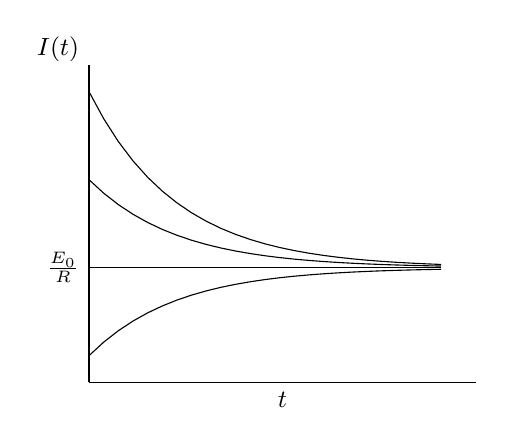
\begin{tikzpicture}
\begin{axis}[small,axis lines*=middle,xmin=0,xlabel={$t$},ylabel={$I(t)$},ylabel style={rotate=-90},ylabel style={at={(axis description cs:0,1.05)}},ytick={1},yticklabels={$\frac{E_0}{R}$},xtick=\empty]
\addplot[domain=0:4]{1+e^(-x)};
\addplot[domain=0:4]{1+0.5*e^(-x)};
\addplot[domain=0:4]{1-0.5*e^(-x)};
\addplot[domain=0:4]{1+0*e^(-x)};
\end{axis}
\end{tikzpicture}
\caption*{سلسلہ وار \عددی{RL} کی رو بالمقابل وقت۔داخلی دباو مستقل مقدار ہے۔}
\end{subfigure}%
\caption{سلسلہ وار \عددی{RL} دور اور اس کی رو۔}
\label{شکل_سادہ_دو_سلسلہ_وار_مزاحمت_امالہ}
\end{figure} 

جوابات:\عددی{LI'+RI=E_0}، \عددی{I=ce^{-\tfrac{R}{L}t}+\tfrac{E_0}{R}} کو شکل \حوالہ{شکل_سادہ_دو_سلسلہ_وار_مزاحمت_امالہ}-ب میں \عددی{c} کی مختلف قیمتوں کے لئے دکھایا گیا ہے۔
\انتہا{سوال}
%======================
\ابتدا{سوال}\شناخت{سوال_سادہ_مزاحمت_امالہ_سائن_نما}
شکل \حوالہ{شکل_سادہ_دو_سلسلہ_وار_مزاحمت_امالہ_سائن_نما}-الف میں \عددی{R=\SI{5}{\ohm}} اور \عددی{L=\SI{1}{\henry}} لیں۔ ابتدائی لمحہ \عددی{t=0} پر \عددی{I(0)=0} لیتے ہوئے \عددی{I(t)} حاصل کریں۔رو کا خط کھینچیں۔
\begin{figure}
\centering
\begin{subfigure}{0.5\textwidth}
\centering
\begin{tikzpicture}
\draw(0,0) to [american voltage source,l={$20\sin 10t $}]++(0,\y) to [resistor,l={$R$}]++(\x,0) to [inductor,l={$L$}]++(0,-\y) to [short](0,0);
\end{tikzpicture}
\caption*{(الف) سلسلہ وار \عددی{RL} دور۔}
\end{subfigure}%
\begin{subfigure}{0.5\textwidth}
\centering
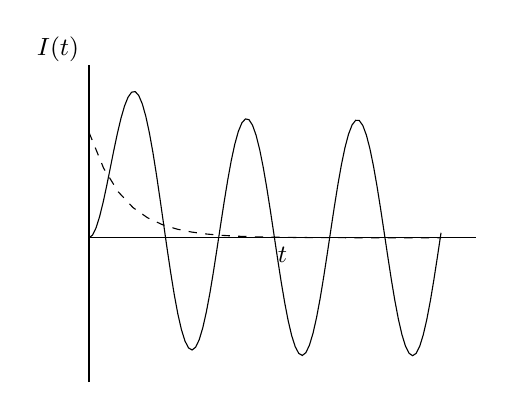
\begin{tikzpicture}
\begin{axis}[small,axis lines*=middle,xmin=0,xlabel={$t$},ylabel={$I(t)$},ylabel style={rotate=-90},ylabel style={at={(axis description cs:0,1.05)}},ytick=\empty,xtick=\empty]
\addplot[domain=0:2,samples=100]{8/5*e^(-5*x)+4/5*sin(180/pi*10*x)-8/5*cos(180/pi*10*x)};
\addplot[dashed,domain=0:2]{8/5*e^(-5*x)};
\end{axis}
\end{tikzpicture}
\caption*{سلسلہ وار \عددی{RL} کی رو بالمقابل وقت۔داخلی دباو مستقل مقدار ہے۔}
\end{subfigure}%
\caption{سوال \حوالہ{سوال_سادہ_مزاحمت_امالہ_سائن_نما} کا دور۔}
\label{شکل_سادہ_دو_سلسلہ_وار_مزاحمت_امالہ_سائن_نما}
\end{figure} 

جواب:\عددی{LI'+RI=E_0\sin \omega t}، 
\عددی{I=\tfrac{8}{5}e^{-5t}+\tfrac{4}{5}\sin 10t-\tfrac{8}{5}\cos 10t}
\انتہا{سوال}
%=============================
\ابتدا{سوال}
شکل \حوالہ{شکل_سادہ_دو_سلسلہ_وار_مزاحمت_امالہ_سائن_نما}-الف میں \عددی{R=\SI{10}{\ohm}} اور \عددی{L=\SI{2}{\henry}} لیں۔برقرار حل رو دریافت کریں۔دباو کے حوالے سے رو کا زاویہ کتنا ہے۔داخلی دباو اور برقرار رو کے خط کھینچیں۔

\begin{figure}
\centering
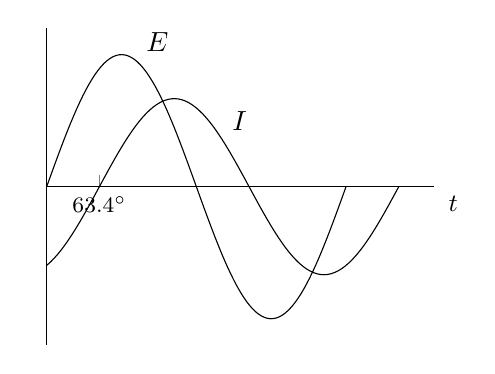
\begin{tikzpicture}
\begin{axis}[small,axis lines*=middle,xlabel={$t$},xlabel style={at={(axis description cs:1.05,0.5)}},ylabel=\empty,ylabel style={rotate=-90},ytick=\empty,xmin=0,xtick={63.4},xticklabels={$63.4^{\circ}$}]
\addplot[domain=0:360,samples=100]{1.5*sin(x)}node[pos=0.3,above right]{$E$};
\addplot[domain=0:423.4,samples=100]{sin(x-63.4)}node[pos=0.5,above right]{$I$};
\end{axis}
\end{tikzpicture}
\caption{\عددی{RL} دور میں دباو سے برقرار رو پیچھے رہتی ہے۔}
\label{شکل_سوال_مزاحمتی_برق_گیر_آگے_زاویہ}
\end{figure}%

جواب:\عددی{I=\tfrac{2}{\sqrt{5}}\sin(10t-1.107)}؛ داخلی دباو سے رو \عددی{63.4^{\circ}} زاویہ پیچھے ہے۔\عددی{RL} دور میں داخلی دباو سے رو \عددی{0^{\circ}} تا \عددی{90^{\circ}} \اصطلاح{پیچھے} ہی رہتی ہے۔شکل \حوالہ{شکل_سوال_مزاحمتی_برق_گیر_آگے_زاویہ} میں دونوں خطوط دکھائے گئے ہیں۔
\انتہا{سوال}
%============================
\ابتدا{سوال}\شناخت{سوال_سادہ_دو_سلسلہ_وار_خصوصی_ب}
سلسلہ وار \عددی{LC} دور میں \عددی{L=\SI{2}{\henry}} اور \عددی{C=\SI{0.02}{\farad}} ہیں۔\عددی{R=0} ہونے کی ناطے \عددی{LC} دور بلا تقصیر ہو گا۔یوں \عددی{LC} نظام بلا تقصیر اسپرنگ اور کمیت  کی نظام کی طرح ہے۔ اس دور کا داخلی دباو \عددی{E(t)=\sin 5t} ہے۔ابتدائی لمحہ \عددی{t=0} پر رو اور برق گیر میں ذخیرہ بار دونوں صفر کے برابر ہیں۔رو کی عمومی مساوات حاصل کریں۔

جواب:\عددی{I(t)=\cos 5t-\cos 100t} 
\انتہا{سوال}
%=========================

سوال \حوالہ{سوال_سادہ_دو_عمومی_سلسلہ_وار_ادوار_الف} تا سوال \حوالہ{سوال_سادہ_دو_عمومی_سلسلہ_وار_ادوار_ب}  شکل \حوالہ{شکل_سادہ_دو_سلسلہ_وار_دور_الف} کے سلسلہ وار \عددی{RLC} دور پر مبنی ہیں۔ان کی برقرار حال رو دریافت کریں۔

%======================
\ابتدا{سوال}\شناخت{سوال_سادہ_دو_عمومی_سلسلہ_وار_ادوار_الف}\quad
$R=\SI{6}{\ohm}, \quad L=\SI{0.4}{\henry}, \quad C=\SI{0.1}{\farad}, \quad E=100\sin 2t\,\si{\volt}$\\
جواب:\عددی{I=13.65\sin(2t+0.611)\,\si{\ampere}}
\انتہا{سوال}
%=========================
\ابتدا{سوال}\quad
$R=\SI{6}{\ohm}, \quad L=\SI{0.4}{\henry}, \quad C=\SI{0.1}{\farad}, \quad E=100\,\si{\volt}$\\
جواب:\عددی{I=\SI{0}{\ampere}}
\انتہا{سوال}
%=========================
\ابتدا{سوال}\quad
$R=\SI{6}{\ohm}, \quad L=\SI{0.4}{\henry}, \quad C=\SI{0.1}{\farad}, \quad E=100\sin 5t\,\si{\volt}$\\
جواب:\عددی{I=\tfrac{50}{3}\sin 5t\,\si{\ampere}}
\انتہا{سوال}
%=========================
\ابتدا{سوال}\quad
$R=\SI{6}{\ohm}, \quad L=\SI{0.4}{\henry}, \quad C=\SI{0.1}{\farad}, \quad E=100\sin 7t\,\si{\volt}$\\
جواب:\عددی{I=16.25\sin (7t-0.225)\,\si{\ampere}}
\انتہا{سوال}
%=========================
\ابتدا{سوال}\quad
$R=\SI{2}{\ohm}, \quad L=\SI{0.8}{\henry}, \quad C=\SI{1.2}{\farad}, \quad E=50\cos 10t\,\si{\volt}$\\
جواب:\عددی{I=5.9\sin 10t+1.5\cos 10t\,\si{\ampere}}
\انتہا{سوال}
%=========================
\ابتدا{سوال}\quad
$R=\SI{1}{\ohm}, \quad L=\SI{0.5}{\henry}, \quad C=\SI{1.5}{\farad}, \quad E=10\cos t\,\si{\volt}$\\
جواب:\عددی{I=-1.6\sin t+9.7\cos t\,\si{\ampere}}
\انتہا{سوال}
%=========================
\ابتدا{سوال}\quad
$R=\SI{0.1}{\ohm}, \, L=\SI{0.2}{\henry}, \, C=\SI{0.01}{\farad}, \quad E=20\sin 10t+10\sin 100t\,\si{\volt}$\\
جواب:\عددی{I=0.003\sin 100t-0.526\cos 100t+0.031\sin 10t+2.5\cos 10t\,\si{\ampere}}
\انتہا{سوال}
%=========================
\ابتدا{سوال}\شناخت{سوال_سادہ_دو_عمومی_سلسلہ_وار_ادوار_ب}
اسپرنگ اور  کمیت کے نظام میں کم قصری، فاصل قصری اور زیادہ قصری صورت پائے گئے۔سلسلہ وار \عددی{RLC} دور میں کم قصری، فاصل قصری اور زیادہ قصری صورت کے شرائط معلوم کریں۔

جوابات:کم قصری صورت \عددی{R^2<\tfrac{4L}{C}} دیتی ہے، جبکہ فاصل قصری صورت میں \عددی{R^2=\tfrac{4L}{C}} اور زیادہ قصری صورت میں
 \عددی{R^2>\tfrac{4L}{C}} ہو گا۔
\انتہا{سوال}
%========================

سوال \حوالہ{سوال_سادہ_دو_عمومی_سلسلہ_وار_مخصوص_الف} تا سوال \حوالہ{سوال_سادہ_دو_عمومی_سلسلہ_وار_مخصوص_ب} ابتدائی قیمت مسئلے ہیں جن میں ابتدائی رو اور برق گیر میں ذخیرہ ابتدائی بار صفر ہیں۔ان کی مخصوص حل حاصل کریں۔

%========================
\ابتدا{سوال}\شناخت{سوال_سادہ_دو_عمومی_سلسلہ_وار_مخصوص_الف}\quad 
$R=\SI{0.1}{\ohm}, \, L=\SI{0.22}{\henry}, \, C=\SI{0.1}{\farad}, \quad E=36\sin 15t\,\si{\volt}$\\
جواب:\عددی{I=0.52\sin 15t-13.65\cos 15t+e^{-\tfrac{5}{22}t}(-0.69\sin 6.74t+13.65\cos 6.74t)\,\si{\ampere}}
\انتہا{سوال}
%========================= 
\ابتدا{سوال}\quad 
$R=\SI{2}{\ohm}, \, L=\SI{0.1}{\henry}, \, C=\SI{0.1}{\farad}, \quad E=10\sin 100t\,\si{\volt}$\\
جواب:\عددی{I=0.196\sin 100t-0.97\cos 100t+e^{-10t}(0.97-9.9t)\,\si{\ampere}}
\انتہا{سوال}
%========================= 
\ابتدا{سوال}\شناخت{سوال_سادہ_دو_عمومی_سلسلہ_وار_مخصوص_ب}\quad 
$R=\SI{4}{\ohm}, \, L=\SI{0.4}{\henry}, \, C=\SI{0.2}{\farad}, \quad E=5\sin 25t\,\si{\volt}$\\
جواب:\عددی{I=0.179\sin 25t-0.437\cos 25t-0.103e^{-1.46t}+0.541e^{-8.54t}\,\si{\ampere}}
\انتہا{سوال}
%========================= 
%==========================


\حصہ{متعین متغیرات بدلنے کے طریقے سے  غیر متجانس خطی سادہ تفرقی مساوات کا حل}\شناخت{سادہ_دو_متغیرات_بدلنے_کا_طریقہ}
پہلے باب میں صفحہ \حوالہصفحہ{مثال_سادہ_درجہ_اول_متغیرات_بدلنے_کا_طریقہ} پر مثال \حوالہ{مثال_سادہ_درجہ_اول_متغیرات_بدلنے_کا_طریقہ} میں ہم نے \اصطلاح{متعین متغیرات بدلنے کے طریقے}\فرہنگ{متعین متغیرات!بدلنے کا طریقہ}\حاشیہب{variation of parameter}\فرہنگ{variation of parameter} سے  تفرقی مساوات کا حل نکالا۔ اس ترکیب\حاشیہد{یہ ترکیب یوسف لوئی لیگرینج سے منسوب ہے۔} سے غیر متجانس خطی سادہ تفرقی مساوات 
\begin{align}\label{مساوات_سادہ_دو_غیر_متجانس_خطی_الف}
y''+p(x)y'+q(x)y=r(x)
\end{align}
کا حل حاصل کرتے ہیں جہاں کھلے وقفے \عددی{I} پر \عددی{p(x)}، \عددی{q(x)} اور \عددی{r(x)} استمراری تفاعل ہیں۔ اس مساوات کو معیاری صورت میں لکھنا ضروری ہے جہاں \عددی{y''} کا عددی سر اکائی \عددی{(1)} کے برابر ہے۔حصہ \حوالہ{حصہ_سادہ_دو_وجودیت_یکتائی_ورونسکی} میں ہم نے دیکھا کہ مساوات \حوالہ{مساوات_سادہ_دو_غیر_متجانس_خطی_الف} کے مطابقتی متجانس مساوات کے عمومی حل \عددی{y_h} اور مساوات \حوالہ{مساوات_سادہ_دو_غیر_متجانس_خطی_الف} کے کسی بھی مخصوص حل \عددی{y_p} کا مجموعہ  اس غیر متجانس مساوات کا عمومی حل دیتا ہے۔سادہ \عددی{r(x)} کی صورت میں \اصطلاح{نا معلوم عددی سر کی ترکیب} استعمال کرتے ہوئے \عددی{y_p} حاصل کی جا سکتی ہے۔اس ترکیب پر حصہ \حوالہ{حصہ_سادہ_دو_غیر_متجانس} میں غور کیا گیا جبکہ حصہ \حوالہ{حصہ_سادہ_دو_جبری_ارتعاش} اور حصہ \حوالہ{حصہ_سادہ_دو_برقی_ادوار} میں اس کا استعمال کیا گیا۔

نا معلوم عددی سر کی ترکیب ان \عددی{r(x)} کے لئے قابل استعمال ہے جن کے تفرق، اصل تفاعل کی صورت رکھتے ہوں مثلاً سائن نما تفاعل، قوت نمائی  تفاعل اور \عددی{x^n} تفاعل۔اس کے برعکس \اصطلاح{متعین متغیرات بدلنے کا طریقہ} زیادہ مشکل تفاعل کے لئے کار آمد ہے۔اس ترکیب کے تحت مساوات \حوالہ{مساوات_سادہ_دو_غیر_متجانس_خطی_الف} کا مخصوص حل
\begin{align}\label{مساوات_سادہ_دو_غیر_متجانس_خطی_ب}
y_p(t)=-y_1\int \frac{y_2 r}{W}\dif x+y_2\int \frac{y_1 r}{W}\dif x
\end{align}
ہے جہاں \عددی{y_1} اور \عددی{y_2} ،مطابقتی متجانس مساوات
\begin{align}\label{مساوات_سادہ_دو_غیر_متجانس_خطی_پ}
y''+p(x)y'+q(x)y=0
\end{align}
 کے حل کی اساس ہیں اور \عددی{W} ان کی \اصطلاح{ورونسکی} [حصہ \حوالہ{حصہ_سادہ_دو_وجودیت_یکتائی_ورونسکی} دیکھیں] ہے۔
\begin{align}\label{مساوات_سادہ_دو_غیر_متجانس_خطی_ت}
W=y_1y_2'-y_2y_1'
\end{align}

مساوات \حوالہ{مساوات_سادہ_دو_غیر_متجانس_خطی_الف} میں متغیر عددی سر کی صورت میں مساوات \حوالہ{مساوات_سادہ_دو_غیر_متجانس_خطی_ب} کے تکملات عموماً مشکلات  پیش کرتے ہیں لہٰذا جہاں ممکن ہو وہاں نا معلوم عددی سر کی ترکیب استعمال کریں۔مساوات \حوالہ{مساوات_سادہ_دو_غیر_متجانس_خطی_ب} کے حصول سے پہلے ایک مثال دیکھتے ہیں جہاں نا معلوم عددی سر کی ترکیب قابل استعمال نہیں ہے لہٰذا موجودہ ترکیب ہی استعمال کی جائے گی۔
%===============================

\ابتدا{مثال}\شناخت{مثال_سادہ_دو_متعین_متغیرات_تبدیلی}
درج ذیل غیر متجانس خطی سادہ تفرقی مساوات کا عمومی حل دریافت کریں۔
\begin{align*}
y''+y=\cosec x
\end{align*}

حل:کسی بھی کھلے وقفے پر متجانس سادہ تفرقی مساوات کی اساس \عددی{y_1=\cos x} اور \عددی{y_2=\sin x} ہیں جن سے ورونسکی لکھتے ہیں۔
\begin{align*}
W=\cos^2 x-\sin x(\sin x)=1
\end{align*} 
مساوات \حوالہ{مساوات_سادہ_دو_غیر_متجانس_خطی_ب} سے \عددی{y_p} حاصل کرتے ہیں
\begin{gather}
\begin{aligned}\label{مساوات_سادہ_دو_مثال_متعین_متغیرات_تبدیلی}
y_p(t)&=-\cos x\int \sin x \cosec x\dif x+\sin x\int \cos x \cosec x\dif x\\
&=-x\cos x+\sin x\ln\abs{\sin x}
\end{aligned}
\end{gather}
جہاں تکمل کے مستقل صفر چننے گئے ہیں۔
\begin{figure}
\centering
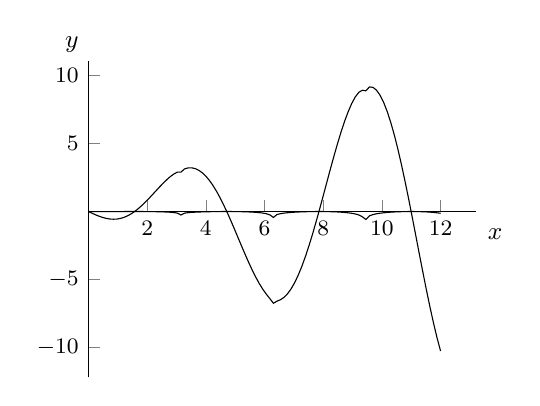
\begin{tikzpicture}
\begin{axis}[small,axis lines*=middle,xlabel={$x$},xlabel style={at={(axis description cs:1.05,0.5)}},ylabel={$y$},ylabel style={rotate=-90},ylabel style={at={(axis description cs:0,1.05)}},xmin=0]
\addplot[domain=0:12,samples=100]{-x*cos(180/pi*x)+sin(x)*ln(abs(sin(180/pi*x)))};
\addplot[domain=0:12,samples=100]{sin(x)*ln(abs(sin(180/pi*x)))};
\end{axis}
\end{tikzpicture}
\caption{مثال \حوالہ{مثال_سادہ_دو_متعین_متغیرات_تبدیلی} کے خطوط۔}
\label{شکل_مثال_سادہ_دو_متعین_متغیرات_تبدیلی}
\end{figure}

شکل \حوالہ{شکل_مثال_سادہ_دو_متعین_متغیرات_تبدیلی} میں \عددی{y_p} اور اس کا دوسرا جزو دکھائے گئے ہیں۔\عددی{y_p} کا دوسرا جزو اتنا کم ہے کہ حقیقتاً پہلا جزو \عددی{-x\cos x} ہی \عددی{y_p} کی قیمت تعین کرتا ہے۔غیر متجانس تفرقی مساوات کا عمومی حل \عددی{y_h=c_1y_1+c_2y_2} اور \عددی{y_p} کا مجموعہ ہو گا۔
\begin{align}\label{مساوات_سادہ_دو_مثال_متعین_متغیرات_تبدیلی_ب}
y=y_h+y_p=(c_1-x)\cos x+(c_2+\ln\abs{\sin x})\sin x
\end{align}
مساوات \حوالہ{مساوات_سادہ_دو_مثال_متعین_متغیرات_تبدیلی} میں تکمل لیتے ہوئے تکمل کے مستقل \عددی{a} اور \عددی{b} بھی شامل کرتے ہوئے
\begin{align*}
y_p(t)&=-\cos x\int \sin x \cosec x\dif x+\sin x\int \cos x \cosec x\dif x\\
&=-\cos x(x+a)+\sin x(\ln\abs{\sin x}+b)
\end{align*}
ملتا ہے۔مساوات \حوالہ{مساوات_سادہ_دو_مثال_متعین_متغیرات_تبدیلی_ب} کے ساتھ موازنہ کرنے سے معلوم ہوتا ہے کہ یہ از خود عمومی حل ہے۔

غیر متجانس تفرقی مساوات \حوالہ{مساوات_سادہ_دو_غیر_متجانس_خطی_الف} کا عمومی حل  مساوات \حوالہ{مساوات_سادہ_دو_غیر_متجانس_خطی_ب} میں تکملات کے مستقل شامل کرتے ہوئے حاصل کیا جا سکتا ہے۔

\انتہا{مثال}
%===========================

\جزوحصہء{متعین متغیرات بدلنے  کے طریقے کا حصول}
اس ترکیب میں متجانس تفرقی مساوات کے حل
\begin{align*}
 y_h(x)=c_1y_1(x)+c_2y_2(x)
\end{align*}
میں مستقل (یعنی متعین متغیرات) \عددی{c_1} اور \عددی{c_2}  کی جگہ نا معلوم تفاعل \عددی{u(x)} اور \عددی{v(x)} پر کئے جاتے ہیں۔اسی لئے اس کو متعین متغیرات بدلنے کا طریقہ کہتے ہیں۔\عددی{u(x)} اور \عددی{v(x)} کی ایسی قیمتیں چننی جاتی ہیں کہ
\begin{align}\label{مساوات_سادہ_دو_غیر_متجانس_خطی_ٹ}
y_p(x)=u(x)y_1(x)+v(x)y_2(x)
\end{align}
غیر متجانس تفرقی مساوات \حوالہ{مساوات_سادہ_دو_غیر_متجانس_خطی_الف} کا مخصوص حل ہو۔حصہ \حوالہ{حصہ_سادہ_دو_وجودیت_یکتائی_ورونسکی} میں مسئلہ \حوالہ{مسئلہ_سادہ_دو_وجودیت_الف} کے تحت کھلے وقفہ \عددی{I} پر استمراری \عددی{p} اور \عددی{q} کی صورت میں اس وقفے پر \عددی{y_h} موجود ہو گا۔جبری تفاعل \عددی{r} کے استمراری ہونے کی ضرورت جلد پیش آئے گی۔

مساوات \حوالہ{مساوات_سادہ_دو_غیر_متجانس_خطی_ٹ} اور اس کے تفرق کو مساوات \حوالہ{مساوات_سادہ_دو_غیر_متجانس_خطی_الف} میں پر کرتے ہوئے \عددی{u} اور \عددی{v} دریافت کرتے ہیں۔مساوات \حوالہ{مساوات_سادہ_دو_غیر_متجانس_خطی_ٹ} کا تفرق لکھتے ہیں۔
\begin{align*}
y'_p=u'y_1+uy'_1+v'y_2+vy'_2
\end{align*}
ہم ایسی \عددی{u} اور \عددی{v} دریافت کر سکتے ہیں کہ \عددی{y_p} غیر متجانس تفرق مساوات پر پورا اترتا ہو جبکہ \عددی{u} اور \عددی{v} درج ذیل مساوات پر پورا اترتے ہوں۔
\begin{align}\label{مساوات_سادہ_دو_تبدیلی_متغیرات_الف}
u'y_1+v'y_2=0
\end{align}
یوں \عددی{y'_p} نسبتاً آسان صورت اختیار کرتی ہے
\begin{align}\label{مساوات_سادہ_دو_غیر_متجانس_خطی_ث}
y'_p=uy'_1+vy'_2
\end{align}
جس کا تفرق لیتے ہوئے \عددی{y''_p} کی مسوات ملتی ہے۔
\begin{align}\label{مساوات_سادہ_دو_غیر_متجانس_خطی_ج}
y''_p=u'y'_1+uy''_1+v'y'_2+vy''_2
\end{align}
مساوات \حوالہ{مساوات_سادہ_دو_غیر_متجانس_خطی_ٹ}، مساوات \حوالہ{مساوات_سادہ_دو_غیر_متجانس_خطی_ث} اور مساوات \حوالہ{مساوات_سادہ_دو_غیر_متجانس_خطی_ج} کو مساوات \حوالہ{مساوات_سادہ_دو_غیر_متجانس_خطی_الف} میں پر کرتے  ہوئے
\begin{align*}
(u'y'_1+uy''_1+v'y'_2+vy''_2) +p(uy'_1+vy'_2)+q(uy_1+vy_2)=r
\end{align*}
\عددی{u}، اور \عددی{v} کے عددی سر اکھٹے کرتے ہیں۔
\begin{align*}
u(y''_1+py'_1+qy_1)+v(y''_2+py'_2+qy_2)+u'y'_1+v'y'_2=r
\end{align*}
چونکہ \عددی{y_1} اور \عددی{y_2} متجانس مساوات \حوالہ{مساوات_سادہ_دو_غیر_متجانس_خطی_پ} کے حل ہیں لہٰذا دونوں قوسین صفر کے برابر ہیں اور درج بالا مساوات نسبتاً سادہ صورت اختیار کر لیتی ہے۔
\begin{align}\label{مساوات_سادہ_دو_تبدیلی_متغیرات_ب}
u'y'_1+v'y'_2=r
\end{align}
یہاں مساوات \حوالہ{مساوات_سادہ_دو_تبدیلی_متغیرات_الف} کو دوبارہ پیش کرتے ہیں۔
\begin{align}\label{مساوات_سادہ_دو_تبدیلی_متغیرات_پ}
u'y_1+v'y_2=0
\end{align}
مساوات \حوالہ{مساوات_سادہ_دو_تبدیلی_متغیرات_ب} اور مساوات \حوالہ{مساوات_سادہ_دو_تبدیلی_متغیرات_پ} دو ہمزاد مساوات ہیں جنہیں حل کرتے ہوئے \عددی{u} اور \عددی{v} حاصل کرتے ہیں۔ \عددی{v'} حذف کرنے کی خاطر پہلی مساوات کو \عددی{-y_2} سے اور دوسری مساوات کو \عددی{y'_2} سے ضرب دیتے ہوئے ان کا مجموعہ لیتے ہیں
\begin{align*}
u'(y_1y'_2-y_2y'_1)=-y_2r\quad \implies \quad u'W=-y_2r
\end{align*}
جہاں \عددی{W} مساوات \حوالہ{مساوات_سادہ_دو_غیر_متجانس_خطی_ت}  ہے۔اسی طرح \عددی{u'} حذف کرنے کی خاطر  پہلی مساوات کو \عددی{y_1} اور دوسری کو \عددی{-y_1'} سے ضرب دیتے ہوئے ان کا مجموعہ لیتے ہیں۔
\begin{align*}
v'(y_1y'_2-y_2y'_1)=y_1r\quad \implies \quad v'W=y_1r
\end{align*}
چونکہ \عددی{y_1} اور \عددی{y_2} حل کی اساس ہیں لہٰذا حصہ \حوالہ{حصہ_سادہ_دو_وجودیت_یکتائی_ورونسکی} میں مسئلہ \حوالہ{مسئلہ_سادہ_دو_حل_تابع_غیر_تابع} کے تحت \عددی{W \ne 0} ہو گا۔اس طرح درج بالا مساوات کو \عددی{W} سے تقسیم کیا جا سکتا ہے جس سے
\begin{align*}
u'=-\frac{y_2r}{W}, \quad v'=\frac{y_1r}{W}
\end{align*}
ملتے ہیں۔تکمل لیتے ہوئے \عددی{u} اور \عددی{v} حاصل ہوتے ہیں۔
\begin{align*}
u=-\int \frac{y_2r}{W} \dif x, \quad v=\int \frac{y_1r}{W} \dif x
\end{align*}
چونکہ کھلے وقفہ \عددی{I} پر \عددی{r} استمراری تفاعل ہے لہٰذا درج بالا تکملات موجود ہیں۔ حاصل \عددی{u} اور \عددی{v} کو مساوات \حوالہ{مساوات_سادہ_دو_غیر_متجانس_خطی_ٹ} میں پر کرتے ہوئے مساوات \حوالہ{مساوات_سادہ_دو_غیر_متجانس_خطی_ب} حاصل ہوتا ہے۔
\begin{align*}
y_p(x)=-y_1\int \frac{y_2r}{W} \dif x+y_2\int \frac{y_1r}{W} \dif x
\end{align*}
%================================
%===================================

\حصہء{سوالات}
مساوات \حوالہ{سوال_سادہ_دو_متعین_متغیرات_کے_بدلتے_ہوئے_الف} تا مساوات \حوالہ{سوال_سادہ_دو_متعین_متغیرات_کے_بدلتے_ہوئے_الف} کو متعین متغیرات بدلنے کے طریقے یا نا معلوم عددی سر کی ترکیب سے حل کریں۔

%==================
\ابتدا{سوال}\شناخت{سوال_سادہ_دو_متعین_متغیرات_کے_بدلتے_ہوئے_الف}\quad
$y''+4y=\sec 2x$\\
جواب:\عددی{y_p=A\cos 2x+B\sin 2x+\tfrac{1}{2}x\sin 2x+\tfrac{1}{4}\cos 2x\ln\abs{\cos 2x}}
\انتہا{سوال}
%====================
\ابتدا{سوال}\quad
$y''+4y=\cosec 2x$\\
جواب:\عددی{y_p=A\cos 2x+B\sin 2x-\tfrac{1}{2}x\cos 2x+\tfrac{1}{4}\sin 2x\ln\abs{\sin 2x}}
\انتہا{سوال}
%=============================
\ابتدا{سوال}\quad
$x^2y''-2xy'+2y=x^3\cos x$\\
جواب:\عددی{y_p=c_1x^2+c_2x-x\cos x}
\انتہا{سوال}
%========================
\ابتدا{سوال}\quad
$y''-2y'+2y=e^x\cosec x$\\
جواب:\عددی{y_p=e^x(A\cos x+B\sin x)-xe^x\cos x+e^x\sin x\ln\abs{\sin x}}
\انتہا{سوال}
%========================
\ابتدا{سوال}\quad
$y''+4y=\sin 2x+\cos 2x$\\
جواب:\عددی{y_p=A\cos 2x+B\sin 2x+\tfrac{1}{4}x\sin 2x+\tfrac{1}{8}(1-2x)\cos 2x}
\انتہا{سوال}
%========================
\ابتدا{سوال}\quad
$y''+6y'+9y=\frac{e^{-3x}}{x^2}$\\
جواب:\عددی{y_p=(ax+b)e^{-3x}-e^{-3x}(1+\ln x)}
\انتہا{سوال}
%========================
\ابتدا{سوال}\quad
$y''+2y'+y=\frac{e^{-x}}{x}$\\
جواب:\عددی{y_p=(ax+b)e^{-x}-xe^{-x}(1-\ln x)}
\انتہا{سوال}
%========================
\ابتدا{سوال}\quad
$y''+2y'+y=\frac{e^{-x}}{x^2}$\\
جواب:\عددی{y_p=(ax+b)e^{-x}-e^{-x}(1+\ln x)}
\انتہا{سوال}
%========================
\ابتدا{سوال}\quad
$y''+2y'+y=\frac{e^{-x}}{x^3}$\\
جواب:\عددی{y_p=(ax+b)e^{-x}+\tfrac{e^{-x}}{2x}}
\انتہا{سوال}
%========================
\ابتدا{سوال}\quad
$y''+4y=\sinh 2x$\\
جواب:\عددی{y_p=A\cos 2x+B\sin 2x+\tfrac{1}{8}\sinh 2x}
\انتہا{سوال}
%========================
\ابتدا{سوال}\quad
$y''-2y'+y=28x^{\frac{1}{3}}e^x$\\
جواب:\عددی{y_p=(ax+b)e^x+9x^{\tfrac{7}{3}}e^x}
\انتہا{سوال}
%========================
\ابتدا{سوال}\quad
$y''+2y'+y=e^{-x}\cosec^3 x$\\
جواب:\عددی{y_p=\tfrac{1}{2}e^{-x}\cosec x[(A+B\sin 2x)+(1-A)\cos 2x]}
\انتہا{سوال}
%========================
\ابتدا{سوال}\quad
$x^2y''+6xy'+6y=x$\\
جواب:\عددی{y_p=\tfrac{x}{12}+c_1x^{-2}+c_2x^{-3}}
\انتہا{سوال}
%========================
\ابتدا{سوال}\quad
$x^2y''+7xy'+9y=25x^2$\\
جواب:\عددی{y_p=x^2+c_1x^{-3}+c_2x^{-2}\ln \abs{x}}
\انتہا{سوال}
%========================

